%%% Hlavní soubor. Zde se definují základní parametry a odkazuje se na ostatní části. %%%

%% Verze pro jednostranný tisk:
% Okraje: levý 40mm, pravý 25mm, horní a dolní 25mm
% (ale pozor, LaTeX si sám přidává 1in)
\documentclass[12pt,a4paper]{report}
\setlength\textwidth{145mm}
\setlength\textheight{247mm}
\setlength\oddsidemargin{15mm}
\setlength\evensidemargin{15mm}
\setlength\topmargin{0mm}
\setlength\headsep{0mm}
\setlength\headheight{0mm}
% \openright zařídí, aby následující text začínal na pravé straně knihy
\let\openright=\clearpage

%% Pokud tiskneme oboustranně:
% \documentclass[12pt,a4paper,twoside,openright]{report}
% \setlength\textwidth{145mm}
% \setlength\textheight{247mm}
% \setlength\oddsidemargin{15mm}
% \setlength\evensidemargin{0mm}
% \setlength\topmargin{0mm}
% \setlength\headsep{0mm}
% \setlength\headheight{0mm}
% \let\openright=\cleardoublepage

%% Pokud používáte csLaTeX (doporučeno):
\usepackage{czech}
%% Pokud nikoliv:
%\usepackage[czech]{babel}
%\usepackage[T1]{fontenc}

%% Použité kódování znaků: obvykle latin2, cp1250 nebo utf8:
\usepackage[utf8]{inputenc}

%% Ostatní balíčky
\usepackage{graphicx}
\usepackage{amsthm}

\usepackage{indentfirst}
\usepackage{fancyhdr}
%\usepackage{setspace}
\usepackage{amsmath}
\usepackage{amssymb}
\usepackage{epsfig}
\usepackage[usenames]{color}
%% Balíček hyperref, kterým jdou vyrábět klikací odkazy v PDF,
%% ale hlavně ho používáme k uložení metadat do PDF (včetně obsahu).
%% POZOR, nezapomeňte vyplnit jméno práce a autora.
\usepackage[ps2pdf,unicode]{hyperref}   % Musí být za všemi ostatními balíčky
\hypersetup{pdftitle=Název práce}
\hypersetup{pdfauthor=Jméno Příjmení}

%%% Drobné úpravy stylu

% Tato makra přesvědčují mírně ošklivým trikem LaTeX, aby hlavičky kapitol
% sázel příčetněji a nevynechával nad nimi spoustu místa. Směle ignorujte.
\makeatletter
\def\@makechapterhead#1{
  {\parindent \z@ \raggedright \normalfont
   \Huge\bfseries \thechapter. #1
   \par\nobreak
   \vskip 20\p@
}}
\def\@makeschapterhead#1{
  {\parindent \z@ \raggedright \normalfont
   \Huge\bfseries #1
   \par\nobreak
   \vskip 20\p@
}}
\makeatother

% Toto makro definuje kapitolu, která není očíslovaná, ale je uvedena v obsahu.
\def\chapwithtoc#1{
\chapter*{#1}
\addcontentsline{toc}{chapter}{#1}
}

\begin{document}

% Trochu volnější nastavení dělení slov, než je default.
\lefthyphenmin=2
\righthyphenmin=2

%%% Titulní strana práce

\pagestyle{empty}
\begin{center}

\large

Univerzita Karlova v Praze

\medskip

Matematicko-fyzikální fakulta

\vfill

{\bf\Large BAKALÁŘSKÁ PRÁCE}

\vfill

\centerline{\mbox{
\includegraphics[width=60mm]{img/logo.eps}}}

\vfill
\vspace{5mm}

{\LARGE Lukáš Beran}

\vspace{15mm}

% Název práce přesně podle zadání
{\LARGE\bfseries Studium fyzikálních vlastností nanostruktur pomocí magnetooptických metod.}

\vfill

% Název katedry nebo ústavu, kde byla práce oficiálně zadána
% (dle Organizační struktury MFF UK)
Fyzikální ústav UK

\vfill

\begin{tabular}{rl}

Vedoucí bakalářské práce: & RNDr. Martin Veis Ph.D. \\
\noalign{\vspace{2mm}}
Studijní program: & Fyzika \\
\noalign{\vspace{2mm}}
Studijní obor: & FOF \\
\end{tabular}

\vfill

% Zde doplňte rok
Praha 2013

\end{center}

\newpage

%%% Následuje vevázaný list -- kopie podepsaného "Zadání bakalářské práce".
%%% Toto zadání NENÍ součástí elektronické verze práce, nescanovat.

%%% Na tomto místě mohou být napsána případná poděkování (vedoucímu práce,
%%% konzultantovi, tomu, kdo zapůjčil software, literaturu apod.)

\openright

\noindent
Poděkování.

Rád bych poděkoval především svému vedoucímu RNDr. Martinu Veisovi, Ph.D. za všechnu pomoc a podporu, bez které by vznik této práce nebyl možný. 
Děkuji za spousty hodin, které se mnou, místo v pohodlí domova, trávil v laboratoři a to nejen, když se něco rozbilo.
Dále bych rád poděkoval doc. RNDr. Jiřímu Bokovi, CSc. za konzultace v oblasti programování a nejednu výtečnou radu.

Nakonec bych nerad opomenul poděkování rodině, přátelům a všem blízkým, kteří mě podporovali nejen po dobu psaní této práce, ale celého studia.

\newpage

%%% Strana s čestným prohlášením k bakalářské práci

\vglue 0pt plus 1fill

\noindent
Prohlašuji, že jsem tuto bakalářskou práci vypracoval(a) samostatně a výhradně
s~použitím citovaných pramenů, literatury a dalších odborných zdrojů.

\medskip\noindent
Beru na~vědomí, že se na moji práci vztahují práva a povinnosti vyplývající
ze zákona č. 121/2000 Sb., autorského zákona v~platném znění, zejména skutečnost,
že Univerzita Karlova v Praze má právo na~uzavření licenční smlouvy o~užití této
práce jako školního díla podle §60 odst. 1 autorského zákona.

\vspace{10mm}

\hbox{\hbox to 0.5\hsize{%
V ........ dne ............
\hss}\hbox to 0.5\hsize{%
Podpis autora
\hss}}

\vspace{20mm}
\newpage

%%% Povinná informační strana bakalářské práce

\vbox to 0.5\vsize{
\setlength\parindent{0mm}
\setlength\parskip{5mm}

Název práce:
Studium fyzikálních vlastností nanostruktur pomocí magnetooptických metod.
% přesně dle zadání

Autor:
Lukáš Beran

Katedra:  % Případně Ústav:
Fyzikální ústav UK
% dle Organizační struktury MFF UK

Vedoucí bakalářské práce:
RNDr. Martin Veis Ph.D.
% dle Organizační struktury MFF UK, případně plný název pracoviště mimo MFF UK

Abstrakt:
Metody magentooptické spektroskopie jsou využívány k výzkumu magnetických vlastností materiálů až do nanometrometrových rozměrů díky své vysoké citlivosti 
a bezkontaktní povaze. To ovšem vyžaduje sofistikovaných experimentálních uspořádání náročných na technické vybavení a nastavení optických komponent. Tato práce popisuje základní fyzikální principy Kerrovy magnetooptické spektroskopie. Na základě těchto principů je navrženo a vyvinuto nové, mnohem jednodušší experimentální uspořádání se zkříženými polarizátory. Toto uspořádání vykazuje řádově stejnou citlivost a přesnost měření jako běžně používané modulační metody se kterými je v této práci srovnáváno. Nakonec je toto uspořádání použito ke studiu magnetooptických vlastností vybraných magnetických struktur a tyto vlastnosti jsou diskutovány.    
% abstrakt v rozsahu 80-200 slov; nejedná se však o opis zadání bakalářské práce

Klíčová slova:
Kerrův jev, experimentální metody, nanostruktury
% 3 až 5 klíčových slov

\vss}\nobreak\vbox to 0.49\vsize{
\setlength\parindent{0mm}
\setlength\parskip{5mm}

Title:
Study of the physical properities of nanostructures using magneto-optical methods.
% přesný překlad názvu práce v angličtině

Author:
Lukáš Beran

Department:
Institute of Physics of Charles University
% dle Organizační struktury MFF UK v angličtině

Supervisor:
RNDr. Martin Veis Ph.D.
% dle Organizační struktury MFF UK, případně plný název pracoviště
% mimo MFF UK v angličtině

Abstract:
Magneto-optical spectroscopy methods are used to study magnetic properties of materials down to nanometer dimensions due to its high sensitivity
and non-contact nature. This requires sophisticated experimental setup, advanced technical equipment and precise optical components arrangement. This thesis 
describes the basic physical principles of magneto-optical Kerr spectroscopy. On the basis of these principles is designed and developed a new, much 
simpler experimental setup with crossed polarizers. This arrangement has the same order of sensitivity and accuracy of measurement as commonly 
used modulation techniques to which it is compared in this work. Finally, this arrangement is applied to the study magneto-optical properties 
of selected magnetic structures and these properties are discussed.
% abstrakt v rozsahu 80-200 slov v angličtině; nejedná se však o překlad
% zadání bakalářské práce

Keywords:
Kerr effect, experimental methods, nanostructures
% 3 až 5 klíčových slov v angličtině

\vss}

\newpage

%%% Strana s automaticky generovaným obsahem bakalářské práce. U matematických
%%% prací je přípustné, aby seznam tabulek a zkratek, existují-li, byl umístěn
%%% na začátku práce, místo na jejím konci.

\openright
\pagestyle{plain}
\setcounter{page}{1}
\tableofcontents

%%% Jednotlivé kapitoly práce jsou pro přehlednost uloženy v samostatných souborech
\chapter*{Úvod}
\addcontentsline{toc}{chapter}{Úvod}

\section{Magnetooptické jevy a jejich využití}
Jako první se jevy, kdy látka ovlivňovala šíření světla v závislosti na magnetickém poli, zabýval Faraday. Roku 1845 objevil, že lineárně polarizované světlo stáčí svou rovinu polarizace při průchodu skleněným válcem v magnetickém poli. To mimo jiné vedlo k potvrzení spojitosti světla a magnetismu. K podobnému závěru došel i Kerr, který však narozdíl od Faradaye nezkoumal průchod, ale odtaz světla.

Magnetooptické jevy se dají pozorovat, jak bylo uvedeno výše, buď při průchodu, bebo odrazu, přičemž naším cílem je zkoumání druhého, častěji zavého Kerrova jevu. Co se týče geometrie, máme na výběr ze tří základních konfigurací. Jedná se o polární, longitudiální a transversální. Jejich schěma naleznete na obrázku (\ref{schema geo}). Jakákoliv jiná poloha vektoru magetizace se dá složit z těchto tří příadů. V rámci této práce se budeme zabývat poze polárním Kerrovýj efektem.

\begin{figure}
\begin{center}
    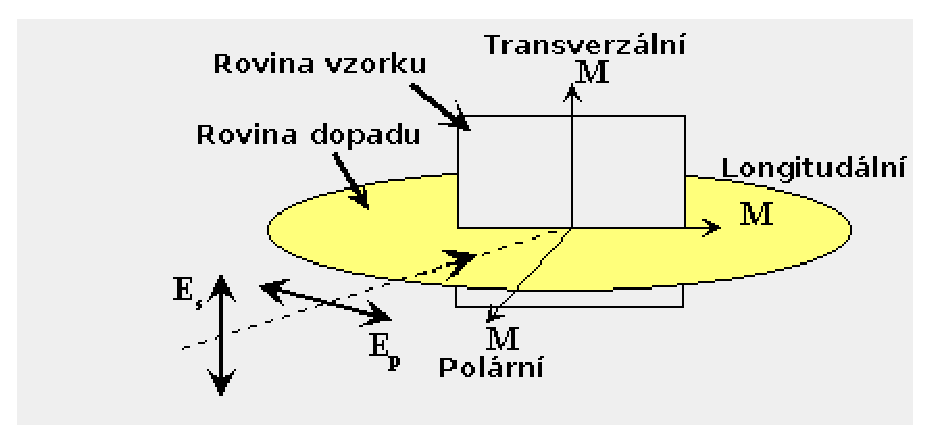
\includegraphics[width=5in]{img/polar.eps}
\end{center}
    \caption{Schéma geometrie Kerrova magnetooptického jevu.}
    \label{schema geo}
\end{figure}

\section{Aplikace magnetoopticky}
Magnetooptika má jakožto velmi široký obor i široké množství uplatnění. Mezi nejznámější patří magnetooptická sektroskopie, umožňující zkoumání struktur o rozměrech řádově nanometrů. Mezi další aplikace patří 3D displaye využívající magnetické nanovrstvy. Pixely těchto displayů se pohybují pod 1 $\mu$m. Jako poslední uvádím magnetooptické izolátory, které propouští světlo pouze jedním směrem. Tyto zařízení jsou nejčastěji používány u výkonných laserů, kde zabraňují návratu svazku zpět do laseru.

\chapter{Polarizace světla}
Polarizace je vlastnost všech harmonických vlnění s možností kmitání ve více jak jednom směru, kterým je například i světlo. V této kapitole popíšeme orientaci elektrického pole v nevodivém homogením izotropním prostředí, kde se světlo šíří. V takovém případě je EM vlna příčná a navíc platí mezi elektrickou intenzitou $\vec{E}$ a magnetickou indukcí $\vec{B}$ vztah
\begin{eqnarray}
\vec{B}=\frac{1}{v}(\vec{s}\times\vec{E}),
\end{eqnarray}
kde $\vec{s}$ je jednotkový vektor ve směru šíření. Díky tomuto vztahu nám tedy popis elektrického pole dá úplnou informaci o celém EM poli. Elektrické pole bylo zvoleno, především kvůli jeho výrazně větším silovým účinkům.
K popisu vektoru elektrické intenzity budeme používat komplexní symboliku. Nejjednoduší případ je rovinná vlna, jejíž předpis můžeme obecně zapsat ve tvaru
\begin{eqnarray}
\vec{E}=Re(\vec{E_0}exp(-i(\omega(t-\frac{\vec{r}\vec{s}}{v})+\varphi))),
\label{rovinna vlna}
\end{eqnarray}
kde $\vec{E_0}$ značí amplitudu vlny, $\omega$ úhlovou frekvenci, $\vec{s}$ jednotkový vektor ve směru šíření a $\varphi$ fázový posun vlny.

Dále si můžeme zvolit soustavu souřadnou tak, aby $\vec{s}$ mířil ve směru osy z. Díky tomu víme, že z-tová složka elektrické intenzity bude nulová a rovnici (\ref{rovinna vlna}) můžeme  přepsat do tvaru
\begin{eqnarray}
\vec{E}(z,t)=E_x\vec{x}+E_y\vec{y} \\
E_x=a_x\cos(\tau+\varphi_x) \label{Ex}\\
E_y=a_y\cos(\tau+\varphi_y) \label{Ey}\\
\tau=\omega(t-\frac{z}{v}))
\end{eqnarray}
Úpravami rovnic (\ref{Ex}) a (\ref{Ey}) a jejich následnými sčítáními můžeme docílit vztahu
\begin{eqnarray}
\left(\frac{E_x}{a_x}\right)^2+\left(\frac{E_y}{a_y}\right)^2-2\frac{E_xE_y}{a_xa_y}\cos(\varphi_y-\varphi_x)=\sin^2(\varphi_y-\varphi_y),
\end{eqnarray}
jenž je rovnicí elispy. Z toho vyplývá, že úplně polarizované světlo má obecně eliptickou polarizace. Tato elispa může být definována různě, proto na obrázku \ref{polarizacni elipsa} naleznete vyznačené nejčastěji užívané parametry. Důležité je, že pro úplný popis potřebujeme parametry čtyři. Pokud nás nezajímá počátek času, vystačíme si jen se třemi. Dále používané parametry po popis polarizace budou
\begin{enumerate}
\item a,b\dots hlavní a vedlejší poloosa
\item $\psi\in[-\pi/2,\pi/2]$\dots azimut
\item $\chi\in[-\pi/2,\pi/2]$\dots úhel elipticity
\end{enumerate}
Úhle elipticity může nabývat i záporných hodnot, protože znaménko v sobě nese informaci o směru otáčení vektoru elektrické intenzity. V naší konvenci máme pro pravotočivé světlo kladné hodnoty a pro levotočivé záporné. Nula odpovídá lineárně polarizovanému světu, kdy vektor elektrické intenzity kmitá pouze v rovině. Tato rovina se nazývá rovinou polarizace. Mezi další význačné polarizace patří kruhově polarizované světlo, kdy $a_x=a_y$ a fázový posun $\varphi=\varphi_y-\varphi_x$ je $\pi/2$ pro pravotočivé a $-\pi/2$ pro levotočivé světlo.

Tento popis polarizace světla je sice úplný, ale pro praktické účely zcela nevhodný. Z toho důvodu vzniklo mnoho formalizmů pro zjednodušení popisu světla a jeho interakci s optickými elementy. Pro náš případ je nejběžněji používaný maticový popis za pomoci takzvaných Jonesových vektorů.

\begin{figure}
\begin{center}
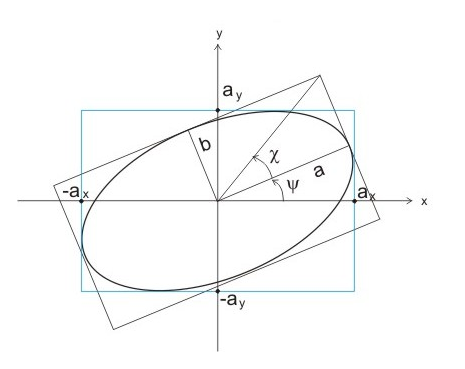
\includegraphics[width=5in]{img/polarelip.eps}
\caption{Polarizační elispa}
\label{polarizacni elipsa}
\end{center}
\end{figure}

\section{Jonesovy vektory a matice}
Tento formalizmus slouží pouze pro popis zcela polarizovaného světla, což by se mohlo zdát velmi omezující, ale pro potřeby této práce s ním bohatě vystačíme. Jak bylo zmíněno výše, rovinnou elektromagneticou vlnu můžeme v komplexní symbolice zapsat
\begin{eqnarray}
\vec{E}(z,t)=E_x\vec{x}+E_y\vec{y} \\
E_x=a_xe^{-i(\omega t-kz+\varphi_x)}=A_xe^{-i(\omega t-kz)}\\
E_y=a_ye^{-i(\omega t-kz+\varphi_y)}=A_ye^{-i(\omega t-kz)},
\end{eqnarray}
kde členy $A_i$ nazveme komplexní obálkou. Díky nim můžeme definovat vektor
\begin{eqnarray}
\vec{J}=\begin{bmatrix} A_x \\ A_y \end{bmatrix},
\end{eqnarray}
který nazveme Jonesovým vektorem polarizace. Tento vektor nese plnou informaci o polarizačním stavu světla. Jako příklad uvádíme pár významných polarizací popsaných za pomoci tohoto formalizmu.
\begin{enumerate}
\item lineárně polarizované v ose x $\begin{bmatrix} 1 \\ 0 \end{bmatrix}$
\item pravotočivě kruhově polarizované světlo $\begin{bmatrix} 1 \\ -i \end{bmatrix}$
\end{enumerate}
Jakoukoliv polarizaci niní můžeme popsat ve tvaru
\begin{eqnarray}
\vec{J}=\alpha_1\vec{J_1}+\alpha_2\vec{J_2}
\end{eqnarray}
kde dvojici vektorů $\vec{J_i}$ volíme ortogonální vzhledem skalárnímu součinu $(\vec{J_1},\vec{J_2})=J_{1x}J_{2x}^*+J_{1y}A_{2y}^*$. Nejběžněji používané  báze jsou
\begin{enumerate}
\item $\vec{J_x} = \begin{bmatrix} 1 \\ 0 \end{bmatrix}$, $\vec{J_y} = \begin{bmatrix} 0 \\ 1 \end{bmatrix}$ \dots báze lineárních polarizací
\item $\vec{J_-} =  \frac{1}{\sqrt{2}} \begin{bmatrix} 1 \\ -i \end{bmatrix}$, $\vec{J_+} = \frac{1}{\sqrt{2}} \begin{bmatrix} 1 \\ +i \end{bmatrix}$ \dots báze kruhových  polarizací
\end{enumerate}
Když máme dobře popsáno světlo, můžeme se přesunout k jeho interakci s optickým prvkem (například čočkou či polarizátorem). Ten můžeme popsat za pomoci matice 2x2. Vektor popisující světlo po interakci s prvkem popsaným maticí $\mathbb{T}$ pak získáme z jednoduché rovnice
\begin{eqnarray}
\vec{J_2}=\mathbb{T}\vec{J_1}.
\end{eqnarray}
Analogicky bychom mohli postupovat pro soustavu $n$ optických prvků, pro kterou bychom získali
\begin{eqnarray}
\vec{J_n}=\mathbb{T}_n...\mathbb{T}_1\vec{J_1}.
\end{eqnarray}
Nyní si uvedeme několik matic popisujících optické prvky, které budou dále použity. Nejprve v bázi lineárních polarizací.
\begin{enumerate}
\item polarizátor natočený o úhel $\alpha$ od osy x $\begin{bmatrix} \cos^2\alpha & \sin\alpha\cos\alpha \\ \sin\alpha\cos\alpha & \sin^2\alpha \end{bmatrix}$
\item fázová destička s fázovým posunem o úhel $\delta$ a rychlou osou ve směru x $\begin{bmatrix} e^{i\frac{\delta}{2}} & 0 \\ 0 & e^{-i\frac{\delta}{2}} \end{bmatrix}$
\item polarizační rotátor stáčející rovinu polarizace o úhle $\vartheta$ $\begin{bmatrix} \cos\vartheta & -\sin\vartheta \\ \sin\vartheta & \cos\vartheta \end{bmatrix}$
\end{enumerate}
a následně v bázi kruhových polarizací
\begin{enumerate}
\item polarizátor natočený o úhel $\alpha$ od osy x  $\frac{1}{2}\begin{bmatrix} 1 & e^{2i\alpha} \\ e^{-2i\alpha} & 1 \end{bmatrix}$
\item fázová destička s fázovým posunem o úhle $\delta$ a rychlou osou ve směru x  $\begin{bmatrix} \cos\frac{\delta}{2} & i\sin\frac{\delta}{2} \\ i\sin\frac{\delta}{2} & \cos\frac{\delta}{2} \end{bmatrix}$
\item polarizační rotátor stáčející rovinu polarizace o úhel $\vartheta$ $\frac{1}{2}\begin{bmatrix} e^{i\vartheta} & 0 \\ 0 & e^{-i\vartheta} \end{bmatrix}$
\end{enumerate}
Velmi užitečný je vztah vztah pro transformaci matice elementu, kterou zíkáme matici odpovídající prvku otočenému o úhel $\vartheta$
\begin{eqnarray}
\mathbb{T}'=\mathbb{R}(\vartheta)\mathbb{TR}(-\vartheta), \\
\mathbb{R}(\vartheta) = \begin{bmatrix} \cos\vartheta & \sin\vartheta \\ -\sin\vartheta & \cos\vartheta \end{bmatrix}.
\end{eqnarray}
Jonesovy matice můžeme také transformovat do bází odpovídající zvojené bázové dvojici Jonesových vektorů. Zde platí vztah podobný jako vztah uvedený výše (Lze na něj nahlížet jako změnu báze na vektory pootočené o úhel $\theta$)
\begin{eqnarray}
\mathbb{T}'=\mathbb{F}^{-1}\mathbb{TF},
\end{eqnarray}
kde $F$ značí matice přechodu z nečárkované báze do báze čárkované. Podrobnosti se dají najít v leckteré učebnici lineární algebry, jako je třeba \cite{Smid}.

\section{Interakce se vzorkem}
V předchozích odstavcích bylo vysvětleno, jak můžeme popsat světlo po průchodu optickou soustavou. Jako poslední nám tedy chybí řešení porblému, kdy se v soustavě vyskytuje neznámý prvek. Tento element můžeme opět popsat Jonesovou maticí, která má obecně čtyři komplexní prvky. Ve skutečnosti jsou tyto matice dvě, protože vzorek se chová jinak pro odraz a jinak pro průchod. Tyto matice si nejprve označíme
\begin{eqnarray}
\mathbb{S}^{sp}_R = \begin{bmatrix} r_{ss} & r_{sp} \\ r_{ps} & r_{ss} \end{bmatrix} \\
\mathbb{S}^{sp}_T = \begin{bmatrix} t_{ss} & t_{sp} \\ t_{ps} & t_{ss} \end{bmatrix} 
\end{eqnarray}
kde $s$ respektive $p$ značí, že používáme za bázi s-polarizované respektive p-polarizované světlo, 
R  reflexi a T trasmisi. Směr $p$ a $s$ polarizace je dán rovinou dopadu, přičemž $p$ je na ni kolmá a $s$ rovnoběžná. 
Pro izotropní materiál bez přítomnost magnetického pole je tato matice diagonální, tedy nedochází k žádné interakci mezi $s$ a $p$ vlnami. 
Po zapnutí magnetického pole jsou nediagonální elemnety obecně nenulové. V případě, že máme geometrii s radiální symetrií, platí vztah
\begin{eqnarray}
\mathbb{R}(\alpha)\mathbb{S}^{sp}_R\mathbb{R}(\alpha)=\mathbb{S}^{sp}_R \\
\mathbb{R}(-\alpha)\mathbb{S}^{sp}_T\mathbb{R}(\alpha)=\mathbb{S}^{sp}_T
\end{eqnarray}
kde $R(\alpha)$ značí matici rotace o úhel $\alpha$.
Z maticových rovnic zíksáme celou řadu vztahů pro maticové elementy
\begin{eqnarray}
r_{ps}&=&r_{sp} \\
t_{ps}&=&-t_{sp} \\
r_{pp}&=&-r_{ss} \\
t_{pp}&=&t_{ss} \\
r_{sp}(-\vec{M})&=&-r_{sp}(\vec{M}) \\
t_{sp}(-\vec{M})&=&-t_{sp}(\vec{M}) \\
r_{ss}(-\vec{M})&=&r_{ss}(\vec{M}) \\
t_{ss}(-\vec{M})&=&r_{ss}(\vec{M}) \\
t_{ss}(-\vec{M})&=&t_{ss}(\vec{M})
\end{eqnarray}
kde $\vec{M}$ značí vektor magnetizace.
V praxi se nepoužívají k popisu maticové elementy, ale veličiny Kerrovy (Faradayovy) rotace ($\theta$)  a elipticity ($\epsilon$), které jsou definovány
\begin{eqnarray}
-\frac{r_{ps}}{r_{ss}}=\Theta_{Ks} \approx \theta_{Ks} -i\epsilon_{Ks} \\
\frac{t_{ps}}{t_{ss}}=\Theta_{Fs} \approx \theta_{Fs}-i\epsilon_{Fs} \\
\frac{r_{sp}}{t_{pp}} = \Theta_{Kp} \approx \theta_{Kp} -i\epsilon_{Kp}\\
-\frac{t{sp}}{t_{pp}} = \Theta_{Fp} \approx \theta_{Fp}-i\epsilon_{Fp}
\end{eqnarray}
Pro kolmý dopad dále platí, že $\Theta_{Ks}=\Theta_{Kp}=\Theta_K$. To samé platí i pro koeficienty transmise. Po normalizaci pak získáme matice popisující vzorek ve tvaru
\begin{eqnarray}
S_R^{sp}&=&\begin{bmatrix}1&-\Theta_K \\ -\Theta_K & -1 \end{bmatrix} \\
S_T^{sp}&=&\begin{bmatrix}1&-\Theta_F \\ \Theta_F& 1 \end{bmatrix}
\end{eqnarray}
Pokud tyto matice transformujeme do báze kruhových polarizací, získáme
\begin{eqnarray}
S_R^{LR}&=&\begin{bmatrix}0 & r_{ss}\\ r_{ss}-ir_{ps}&0\end{bmatrix} \\
S_T^{LR}&=&\begin{bmatrix}t_{ss} & 0 \\ 0& t_{ss}-it_{ps}\end{bmatrix}
\end{eqnarray}

\chapter{EM vlny v anizotropním prostředí}
\section{Vlnová rovnice v anizotropním prostředí}
Vlnová rovnice pro světlo v anizotropním prostředí, tedy homogení nevodivé bez nábojů a proudů, se dá snadno dovodit z Maxwellových rovnic
\begin{eqnarray}
\nabla \times\vec{H} - \frac{\partial\vec{D}}{\partial t} &=& 0 , \label{Max1} \\
\nabla \cdot \vec{D} &=& 0, \label{Max2} \\
\nabla \times \vec{E} + \frac{\partial \vec{B}}{\partial t} &=& 0, \label{Max3}\\
\nabla\cdot\vec{B}&=&0 \label{Max4}
\end{eqnarray}
Na optických frekvencích můžeme počítat, že $\mu_r\approx1$ a tedy platí brát $\mu=\mu_0$. Prostředí je tedy charakterizováno tensorem permitivity $\varepsilon$. Tento tenzor má obecně tvar
\begin{eqnarray}
\varepsilon=
\begin{bmatrix}
\varepsilon_{xx} & \varepsilon_{xy} & \varepsilon_{xz} \\
\varepsilon_{yz}& \varepsilon_{yy}& \varepsilon_{yz} \\
\varepsilon_{zx}& \varepsilon_{zy}& \varepsilon_{zz}
\end{bmatrix}
\end{eqnarray}
Dále vhodné zavést tzv. redukovaný vlnový vektor, který zančíme $\vec{N}$ a je definován
\begin{eqnarray}
\vec{N}=\frac{c}{\omega}\vec{k} = (N_x\vec{i_x}+N_y\vec{i_y}+N_z\vec{i_z})
\end{eqnarray}
Standartní řešení ve tvaru rovinné vlny
\begin{eqnarray}
\vec{E} &=& \vec{E_0}e^{[-i(\omega t-\vec{k}\cdot\vec{r})]}, \\
\vec{B} &=& \vec{B_0}e^{[-i(\omega t-\vec{k}\cdot\vec{r})]}
\end{eqnarray}
dává po dosazení do rovnic (\ref{Max1}) a (\ref{Max2})
\begin{eqnarray}
\vec{k}\times(\vec{k}\times\vec{E}) + \frac{\omega^2}{c^2}\varepsilon\vec{E}=0
\end{eqnarray}
Tuto vektorovou rovnici můžeme rozepsat pro složky vektorů za pomoci Levi-Civitova symbolu $\epsilon$ do tvaru
\begin{eqnarray}
\epsilon_{ijk}k_j\epsilon_{klm}k_lE_m+\frac{\omega^2}{c^2}\varepsilon_{ij}E_j =0
\end{eqnarray}
Postupnou úpravou, která je podrobněji popsána v \cite{Nyvlt} a volbou soustavy souřadné, kde BÚNO $N_x=0$ získáme maticovou rovnici
\begin{eqnarray}
\begin{bmatrix}
\varepsilon_{xx}-N_y^2-N_z^2& \varepsilon_{xy}& \varepsilon_{xz} \\
\varepsilon_{yx}&   \varepsilon_{yy}-N_z^2& \varepsilon_{yz}+N_yN_z\\
\varepsilon_{zx}&   \varepsilon_{zy}+N_yN_z& \varepsilon_{zz}-N_y^2
\end{bmatrix}
\begin{bmatrix}
E_x\\ E_y\\ E_z
\end{bmatrix} = 0
\label{Matic1}
\end{eqnarray}
Pro získání jendoznačných řešení musíme fixovat další parametr, z toho důvodu budeme dále předpokládat znalost komponenty $N_y$, kterou určuje úhel dopadu.

Řešení rovnice (\ref{Matic1}) nebude triviální za předpokladu, že determinant první matice bude nulový. Tak získáme charakteristickou rovnici soustavy pro vlastní honodty $N_z$
\begin{eqnarray}
N_z^4\varepsilon_{zz}+N_z^3[N_y(\varepsilon_{yz}+\varepsilon_{yz})]\\
-N_z^2[\varepsilon_{zz}(\varepsilon_{zz}-N_y^2)+\varepsilon_{zz}(\varepsilon_{xx}-N_y^2)-\varepsilon_{xz}\varepsilon_{zx}-\varepsilon_{yz}\varepsilon_{zy}]\\
-N_z[(\varepsilon_{xx}-N_y^2)(\varepsilon_{yz}+\varepsilon_{zy})-\varepsilon_{xy}\varepsilon_{zx}-\varepsilon_{yx}\varepsilon_{xz}]N_y \\
+\varepsilon_{yy}[(\varepsilon_{xx}-N_y^2)(\varepsilon_{zz}-N_y^2)-\varepsilon_{xz}\varepsilon_{zx}]\\
-\varepsilon_{xy}\varepsilon_{yx}(\varepsilon_{zz}-N_y^2)-\varepsilon_{yz}\varepsilon_{zy}(\varepsilon_{xx}-N_y^2)1\varepsilon_{xy}\varepsilon_{zx}\varepsilon_{yz}+\varepsilon_{yx}\varepsilon_{xz}\varepsilon_{zy}=0
\end{eqnarray}
Řešení jsou tedy čtyři hodnoty $N_z$, které popisují šíření čtyř vlastních polarizací $\vec{e}_j$, kde
\begin{eqnarray}
\vec{e}_j=
\begin{bmatrix}
-\varepsilon_{xy}(\varepsilon_{zz}-N_y^2)+\varepsilon_{xz}(\varepsilon_{zy}+N_yN_{zj} \\
(\varepsilon_{zz}-N_y^2)(\varepsilon_{xx}-N_y^2-N^2_{zj})-\varepsilon_{xz}\varepsilon_{zx} \\
-(\varepsilon_{xx}-N_y^2-N^2_{zj})(\varepsilon_{zy}+N_yN_{zj})+\varepsilon_{zx}\varepsilon_{xy}
\end{bmatrix}
\end{eqnarray}
Tato řešení se při průchodu prostředím nemění, proto jsou vhodnou volbou pro bázi. Libovolné pole pak můžeme zapsat ve tvaru
\begin{eqnarray}
\vec{E}=\sum_{j=1}^2E_{0j}\vec{e_j}e^{i\omega t-i\frac{\omega}{c}\vec{N_j}\cdot\vec{r}}
\label{Rozpis E}
\end{eqnarray}

\section{Šíření světla podél vektoru magnetizace}
V případě, kdy se světlo šíří ve směru směru vektoru magnetizace víme díky symetrii problému, že tezor permitivity má výrazně jednodušší tvar
\begin{eqnarray}
\varepsilon=\begin{bmatrix}\varepsilon_{xx}&  -i\varepsilon_{xy}& 0 \\ i\varepsilon{xy}& \varepsilon_{xx}&  0 \\ 0&0& \varepsilon_{zz}\end{bmatrix}
\label{epsilon polar}
\end{eqnarray}
Díky tomu se rovnice (\ref{Matic1}) výrazně zjednodušší. Ve zkratce, pokud zvolíme $N_y=0$, což odpovídá kolmému dopadu, pak se charakteristická ropvnice redukuje na
\begin{eqnarray}
N_z^4-2\varepsilon_1N_z^2+\varepsilon_1^2-\varepsilon_2^2=0,
\end{eqnarray}
což vede na řešení
\begin{eqnarray}
N_z^2=\varepsilon_1 \pm \varepsilon_2.
\end{eqnarray}
Z čehož získáme řádné módy šíření
\begin{eqnarray}
N_\pm=\sqrt{\varepsilon_1\pm\varepsilon_2}
\end{eqnarray}


\section{Magnetické multivrstvy}
Nyní se budeme zabývat situací, kdy máme několik tenkých anizotropních planpalarelních vrstev na sobě. Formalismus popisující tuto problematiku zavedl Yeh a je podrobně popsán napříkald v \cite{Nyvlt}.

Jak bylo zmíněno, předpokládáme materiál tvořený $m$ vrstvami. Rozhraní mezi vrstvami jsou kolmá na osu z. N-tá vrstva je charakterizovaná tenzorem permitivity $\varepsilon^{(n)}$ a tloušťkou $t_n$. Vlnový vektor $\vec{k}_0$ popisující dopadající vlnu svírá s osou z úhel $\varphi$. Elektrické pole v $n$-té vrstvě pak můžeme, jak bylo popsáno výše, rozložit do řádných módů. Tak získáme pro výsledné pole v každé vrstvě výraz
\begin{eqnarray}
\vec{E}^{(n)}=\sum^4_{j=1}E_{0j}^{(n)}(z_n)\vec{e}_j^{(n)}\mbox{exp}\left\{i\omega t-i\frac{\omega}{c}[N_yy+N_{zj}^{(n)}(z-z_n)]\right\},
\end{eqnarray}
kde $z_n$ značí z-ovou souřadnici rozhraní $n$-té a $(n+1)$-ní vrstvy a $N_{zj}$ komponenty redukovaného vlnového vektoru.

Dále bez odvození uvádíme okrajové podmínky na rozhraní n-té a (n-1)-ní vrstvy. Jedná se o soustavu čtyř rovnic pro $E_x$, $E_y$, $B_y$ a $B_x$
\begin{eqnarray}
\sum^4_{j=1}E_{0j}^{(n-1)}(z_{n-1})\vec{e}_j^{(n-1)}\cdot\vec{i}_x &=& \sum^4_{j=1}E_{0j}^{(n)}(z_n)\vec{e}_j^{(n)}\cdot\vec{i}_x \mbox{exp}\left(i\frac{\omega}{c}N_{zj}^{(n)}t_n\right), \\
\sum^4_{j=1}E_{0j}^{(n-1)}(z_{n-1})\vec{b}_j^{(n-1)}\cdot\vec{i}_y &=& \sum^4_{j=1}E_{0j}^{(n)}(z_n)\vec{b}_j^{(n)}\cdot\vec{i}_y \mbox{exp}\left(i\frac{\omega}{c}N_{zj}^{(n)}t_n\right), \\
\sum^4_{j=1}E_{0j}^{(n-1)}(z_{n-1})\vec{e}_j^{(n-1)}\cdot\vec{i}_y &=& \sum^4_{j=1}E_{0j}^{(n)}(z_n)\vec{e}_j^{(n)}\cdot\vec{i}_y \mbox{exp}\left(i\frac{\omega}{c}N_{zj}^{(n)}t_n\right), \\
\sum^4_{j=1}E_{0j}^{(n-1)}(z_{n-1})\vec{b}_j^{(n-1)}\cdot\vec{i}_x &=& \sum^4_{j=1}E_{0j}^{(n)}(z_n)\vec{b}_j^{(n)}\cdot\vec{i}_x \mbox{exp}\left(i\frac{\omega}{c}N_{zj}^{(n)}t_n\right).
\end{eqnarray}
Tato soustava popisuje lineární transformaci amplitud příslušných modů. Velmi výhodné je její přepsání do maticové rovnice
\begin{eqnarray}
\mathbb{D}^{(n-1)}\vec{E}_0^{(n-1)}(z_{n-1})=\mathbb{D}^{(n)}\mathbb{P}^{(n)}\vec{E}^{(n)}_0(z_n),
\end{eqnarray}
kde čtvrtá komponenta vektoru $\vec{E_0^{(n)}}$ je koeficient $E^{(n)}_{0j}(z_n)$. Prvky propagační matice $\mathbb{P}$ jsou dány
\begin{eqnarray}
\mathbb{P}_{ij}^{(n)}=\delta_{ij} \mbox{exp}\left(i\frac{\omega}{c}N_{zj}^{(n)}t_n\right).
\end{eqnarray}
Řádky dynamické matice $\mathbb{D}$ jsou pak dány komponentami příslušných polarizací
\begin{eqnarray}
\mathbb{D}_{1j}^{(n)}=\vec{e}_j^{(n)}\cdot\vec{i}_x, \\
\mathbb{D}_{2j}^{(n)}=\vec{b}_j^{(n)}\cdot\vec{i}_y, \\
\mathbb{D}_{3j}^{(n)}=\vec{e}_j^{(n)}\cdot\vec{i}_y, \\
\mathbb{D}_{4j}^{(n)}=\vec{b}_j^{(n)}\cdot\vec{i}_x.
\end{eqnarray}
Abychom se nemuseli zabývat obencným řešením těchto rovnic, využijeme toho, že při polární magnetizaci má tenzor permitivity tvar (\ref{epsilon polar}). To vede na zjednodušené rovnice
\begin{eqnarray}
\mathbb{D}_{1j}^{(n)}&=& -\varepsilon_{xy}(\varepsilon_{xx}-N_y^2)+\varepsilon_{xx}N_yN_z, \\
\mathbb{D}_{2j}^{(n)}&=&N_{zj}[-\varepsilon_{xy}^{(n)}(\varepsilon_{zz}^{(n)}-N_y^2)], \\
\mathbb{D}_{3j}^{(n)}&=&(\varepsilon_{zz}^{(n)}-N^2_y(\varepsilon_{xx}^{(n)}-N_y^2-N_{zj}^{(n)2}), \\
\mathbb{D}_{4j}^{(n)}&=&-(\varepsilon_{xx}^{(n)}-N_y^2-N_{zj}^{(n)2})N_{zj}^{(n)}\varepsilon_{zz}^{(n)})
\end{eqnarray}
díky kterým sjme schopni určit celou dynamickou matici.
Pro $m$ vrstev pak získáme výsledný vztah pouhým násobením matic
\begin{eqnarray}
\vec{E}_0^{(0)}(z_0) = [\mathbb{D}^{(0)}]^{-1}\mathbb{D}^{(1)}\mathbb{P}^{(1)}[\mathbb{D}^{(1)}]^{-1}\dots \mathbb{D}^{(m)}\mathbb{P}^{(m)}[\mathbb{D}^{(m)}]^{-1}\mathbb{D}^{(m+1)}\vec{E}_0^{(m+1)}(z_m)\\
=\mathbb{M}\vec{E}_0^{(m+1)}(z_m)
\end{eqnarray}
Z matice $\mathbb{M}$ můžeme následně vypočítat reflexní a trasmisní koeficienty, jako poměr apmlitudy dopadajícího a odraženého, či prošlého pole, s uvážením, že z $E^{(n)}$ nic nedopadá. Ve zkratce získáme vztahy %TODO ověřit
\begin{eqnarray}
r_{12}=\frac{M_{21}M_{33} - M_{23}M_{31}}{M_{11}M_{33}-M_{13}M_{31}}, \\
r_{14}=\frac{M_{41}M_{33}-M_{43}M_{31}}{M_{11}M_{33}-M_{13}M_{31}}, \\
r_{31}=\frac{M_{11}M_{43}-M_{41}M_{13}}{M_{11}M_{33}-M_{13}M_{31}}, \\
r_{32}=\frac{M_{11}M_{23}-M_{21}M_{13}}{M_{11}M_{33}-M_{13}M_{31}}.
\end{eqnarray}
Přičemž platí vztah vázající tyto koeficienty s Jonesovou reflexní maticí
\begin{eqnarray}
\begin{bmatrix}
r_{ss} & r_{sp} \\ r_{ps} & r_{pp} 
\end{bmatrix}
= 
\begin{bmatrix} 
r_{12} &r_{32} \\ -r_{14} & -r_{34} 
\end{bmatrix}
\end{eqnarray}
Analogické vztahy platí i pro transmisní koeficienty. Z obou pak můžeme dopočítat příslušné Kerrovy či Faradayovy koeficienty.

\section{Jednoduchá vrstva}
Pokud máme pouze jednu vrstvu na substrátu, můžeme se vyhnout řešení maticové rovnice a použít vztah
\begin{eqnarray}
\Theta_K=\theta_K-i\epsilon_K=\frac{i\varepsilon_2(1-r^2_{01})\left[(1+r^2_{12}e^{-2i\beta_1})(1-e^{-2i\beta_1})+4i\beta_1e^{-2i\beta_1}\right]}{4\varepsilon_1(1+r_{01}+r_{12}e^{-2i\beta_1})},
\label{teor kerr}
\end{eqnarray}
kde $\beta_1=n_1\frac{\omega}{c}t_1=\sqrt{\varepsilon_1}\frac{E}{\hbar c}t_1$ a $r_{01}$ resp. $r_{12}$ jsou Fresnelovy reflexní koeficienty na prvním resp. druhém rozhraní. Pro kolmý dopad dosadíme
\begin{eqnarray}
r_{ij}=\frac{\sqrt{\varepsilon_j}-\sqrt{\varepsilon_i}}{\sqrt{\varepsilon_j}+\sqrt{\varepsilon_i}}
\end{eqnarray}
Po zdlouhavých úpravách lze tuto rovnici upravit a separovat na výrazy
\begin{eqnarray}
\theta_K&=&K\frac{AC+BD}{C^2+D^2}\\
\epsilon_K&=&K\frac{BC-AD}{C^2+D^2} \\
K&=&\frac{(1-r_{01}^2)\varepsilon_2}{4\varepsilon_1} \\
A&=&s+2r_{12}^2cs-r^2_{12}s+4\beta_1r_{12}c \\
B&=&1-c+4\beta_1r_{12}s+r^2_{12}(c-c^2-s^2) \\
C&=&r_{01}+r_{12}c+r_{01}^2r_{12}c+r_{01}2r_{12}^2c^2-r_{01}r_{12}^2s^2 \\
D&=&r_{12}s+2r_{01}r_{12}^2cs+r_{01}^2r_{12}s \\
c&=&\cos 2\beta_1;\, s=\sin 2\beta_1,
\end{eqnarray}
které jsou o něco použitelnější pro numerický výpočet.

\chapter{Experimentální metody}

\section{Metoda téměř zkřížených polarizátorů}
\subsection{Teorie}
Toto experimentální uspořádání umožňuje rychlé určení Kerrovy rotace a elipsity pro celé spektrum. V našem případě používáme CCD spektometr v kombinaci se širokospektrálním zrojem, který se skládá z halogenové a deuteriové výbojky. To umožňuje proměření celého spektra najednou. Schéma celého experimentu je zobrazeno na obrázku (\ref{Schema TPE}). Ze zdroje je světlo vedeno optickým vláknem do aparatury. Svazek je nejprve kolimován spojnou čočkou. Následně prochází polarizátorem, který je otočen o úhel $\alpha$ od svislé osy a fázovou destičkou s fázovým posuvem $\delta$. Po odrazu na vzorku prochází světlo analyzátorem, který je natočený o úhel $\pi/2$ od svilé osy. Výstupní světlo je zachyceno sběrnou čočkou do optického vlákna, které vede do spektrometru. Za pomoci Jonesova formalizmu můžeme spočítat Jonesův vektor světla dopadajícího na detektor.
\begin{eqnarray}
J=r\begin{bmatrix}0&0\\0&1\end{bmatrix}\begin{bmatrix}1&-\Theta_K\\-\Theta_K&-1\end{bmatrix}\begin{bmatrix}e^{i\frac{\delta}{2}}&0\\0&e^{-i\frac{\delta}{2}}\end{bmatrix}\begin{bmatrix}\cos\alpha\\\sin\alpha\end{bmatrix}\\
=r\begin{bmatrix}0\\-\Theta_Ke^{i\frac{\delta}{2}}\cos\alpha+e^{-i\frac{\delta}{2}}\sin\alpha\end{bmatrix},
\end{eqnarray}
kde $r$ značí reflexní koeficient vzorku. Pro intenzitu světla u sběrné čočky pak máme
\begin{eqnarray}
I\approx\frac{1}{2}JJ^*=\frac{R}{2}(\sin^2\alpha+|\Theta_K|^2\cos^2\alpha+\sin(2\alpha)\mbox{Re}(\Theta_Ke^{i\delta}))
\label{I1}
\end{eqnarray}
Nyní můžeme použít přiblížení pro malé elipsometrické úhly, pro které platí
\begin{eqnarray}
\Theta_K\approx\theta_K-i\epsilon_K
\end{eqnarray}
Výraz (\ref{I1}) se pak redukuje na
\begin{eqnarray}
I\approx\frac{R}{2}(\sin^2\alpha+(\theta_K\cos\delta+\epsilon_K\sin\delta)\sin(2\alpha))
\label{I2}
\end{eqnarray}
V  případě, že $\delta=0$, tedy odebereme fázovou destičku, nám zcela vymizí elipticita. Fitováním naměřených dat v závislost na úhlu natočení polarizátoru $\alpha$ pak můžeme získat přímo rotaci. Pro určení elipticity následně naměříme i hodnoty s fázovou destičkou. V ideáním případě bychom použili půlvlnnou destičku, ale vzhledem k tomu, že její fáze je funkcí vlnové délky, musíme počítat s tím, že fitovaný parametr při druhém měření odpovídá celému výrazu $K=(\theta_K\cos\delta+\epsilon_K\sin\delta)$. Rotaci známe z prvního měření a $\delta$ určíme z kalibrační funkce destičky. Elipticita se nakonec rovná
\begin{eqnarray}
\epsilon_K=(K-\theta_K\cos\delta)/\sin\delta
\end{eqnarray}

Tato závislost předpokádá přesné určení vzájemné polohy polarizátorů. Tu však v praxi neznáme a proto využíváme toho, že platí $\theta_K(M)=-\theta_K(-M)$. kde $M$ značí magnetizaci. Měříme tedy závislosti pro dva opačné proudy procházející magnetem a výsledné nafitované konstanty od sebe odečteme a vydělíme dvěmi.

\begin{figure}
    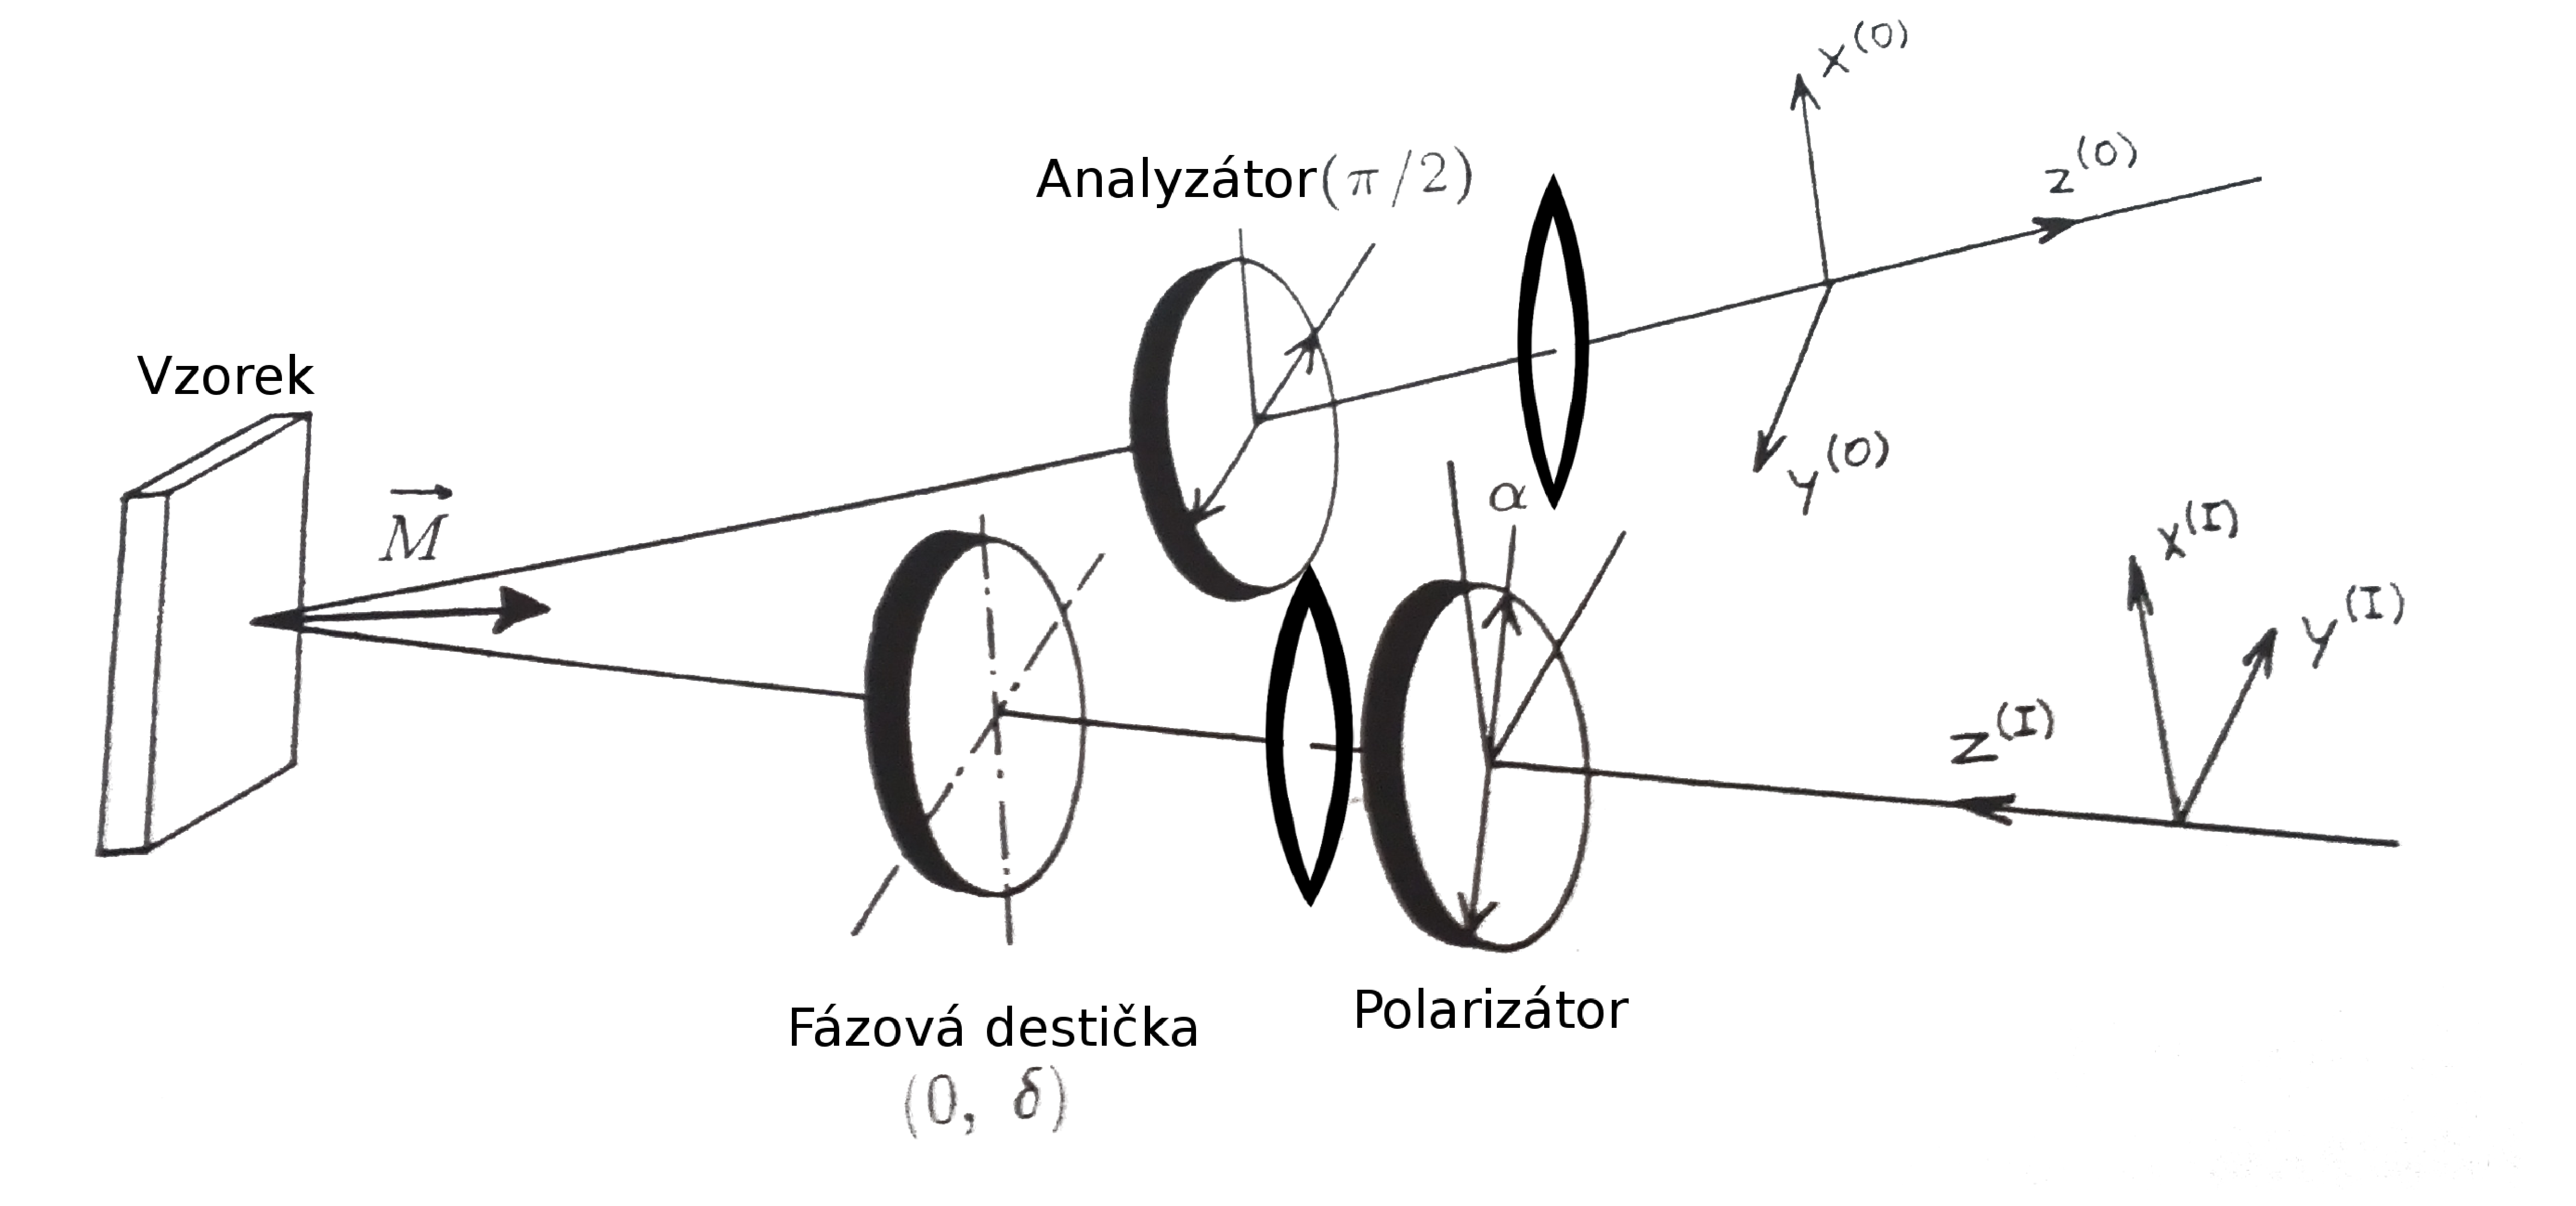
\includegraphics[width=5in]{img/TPEschema.eps}
    \caption{Schéma metody téměř zkřížených polarizátorů.}
    \label{Schema TPE}
\end{figure}

\subsection{Použitá zařízení}
Fotografii celé aparatury můžete vidět na obrázku (\ref{TPE photo}).

\begin{figure}
\begin{center}
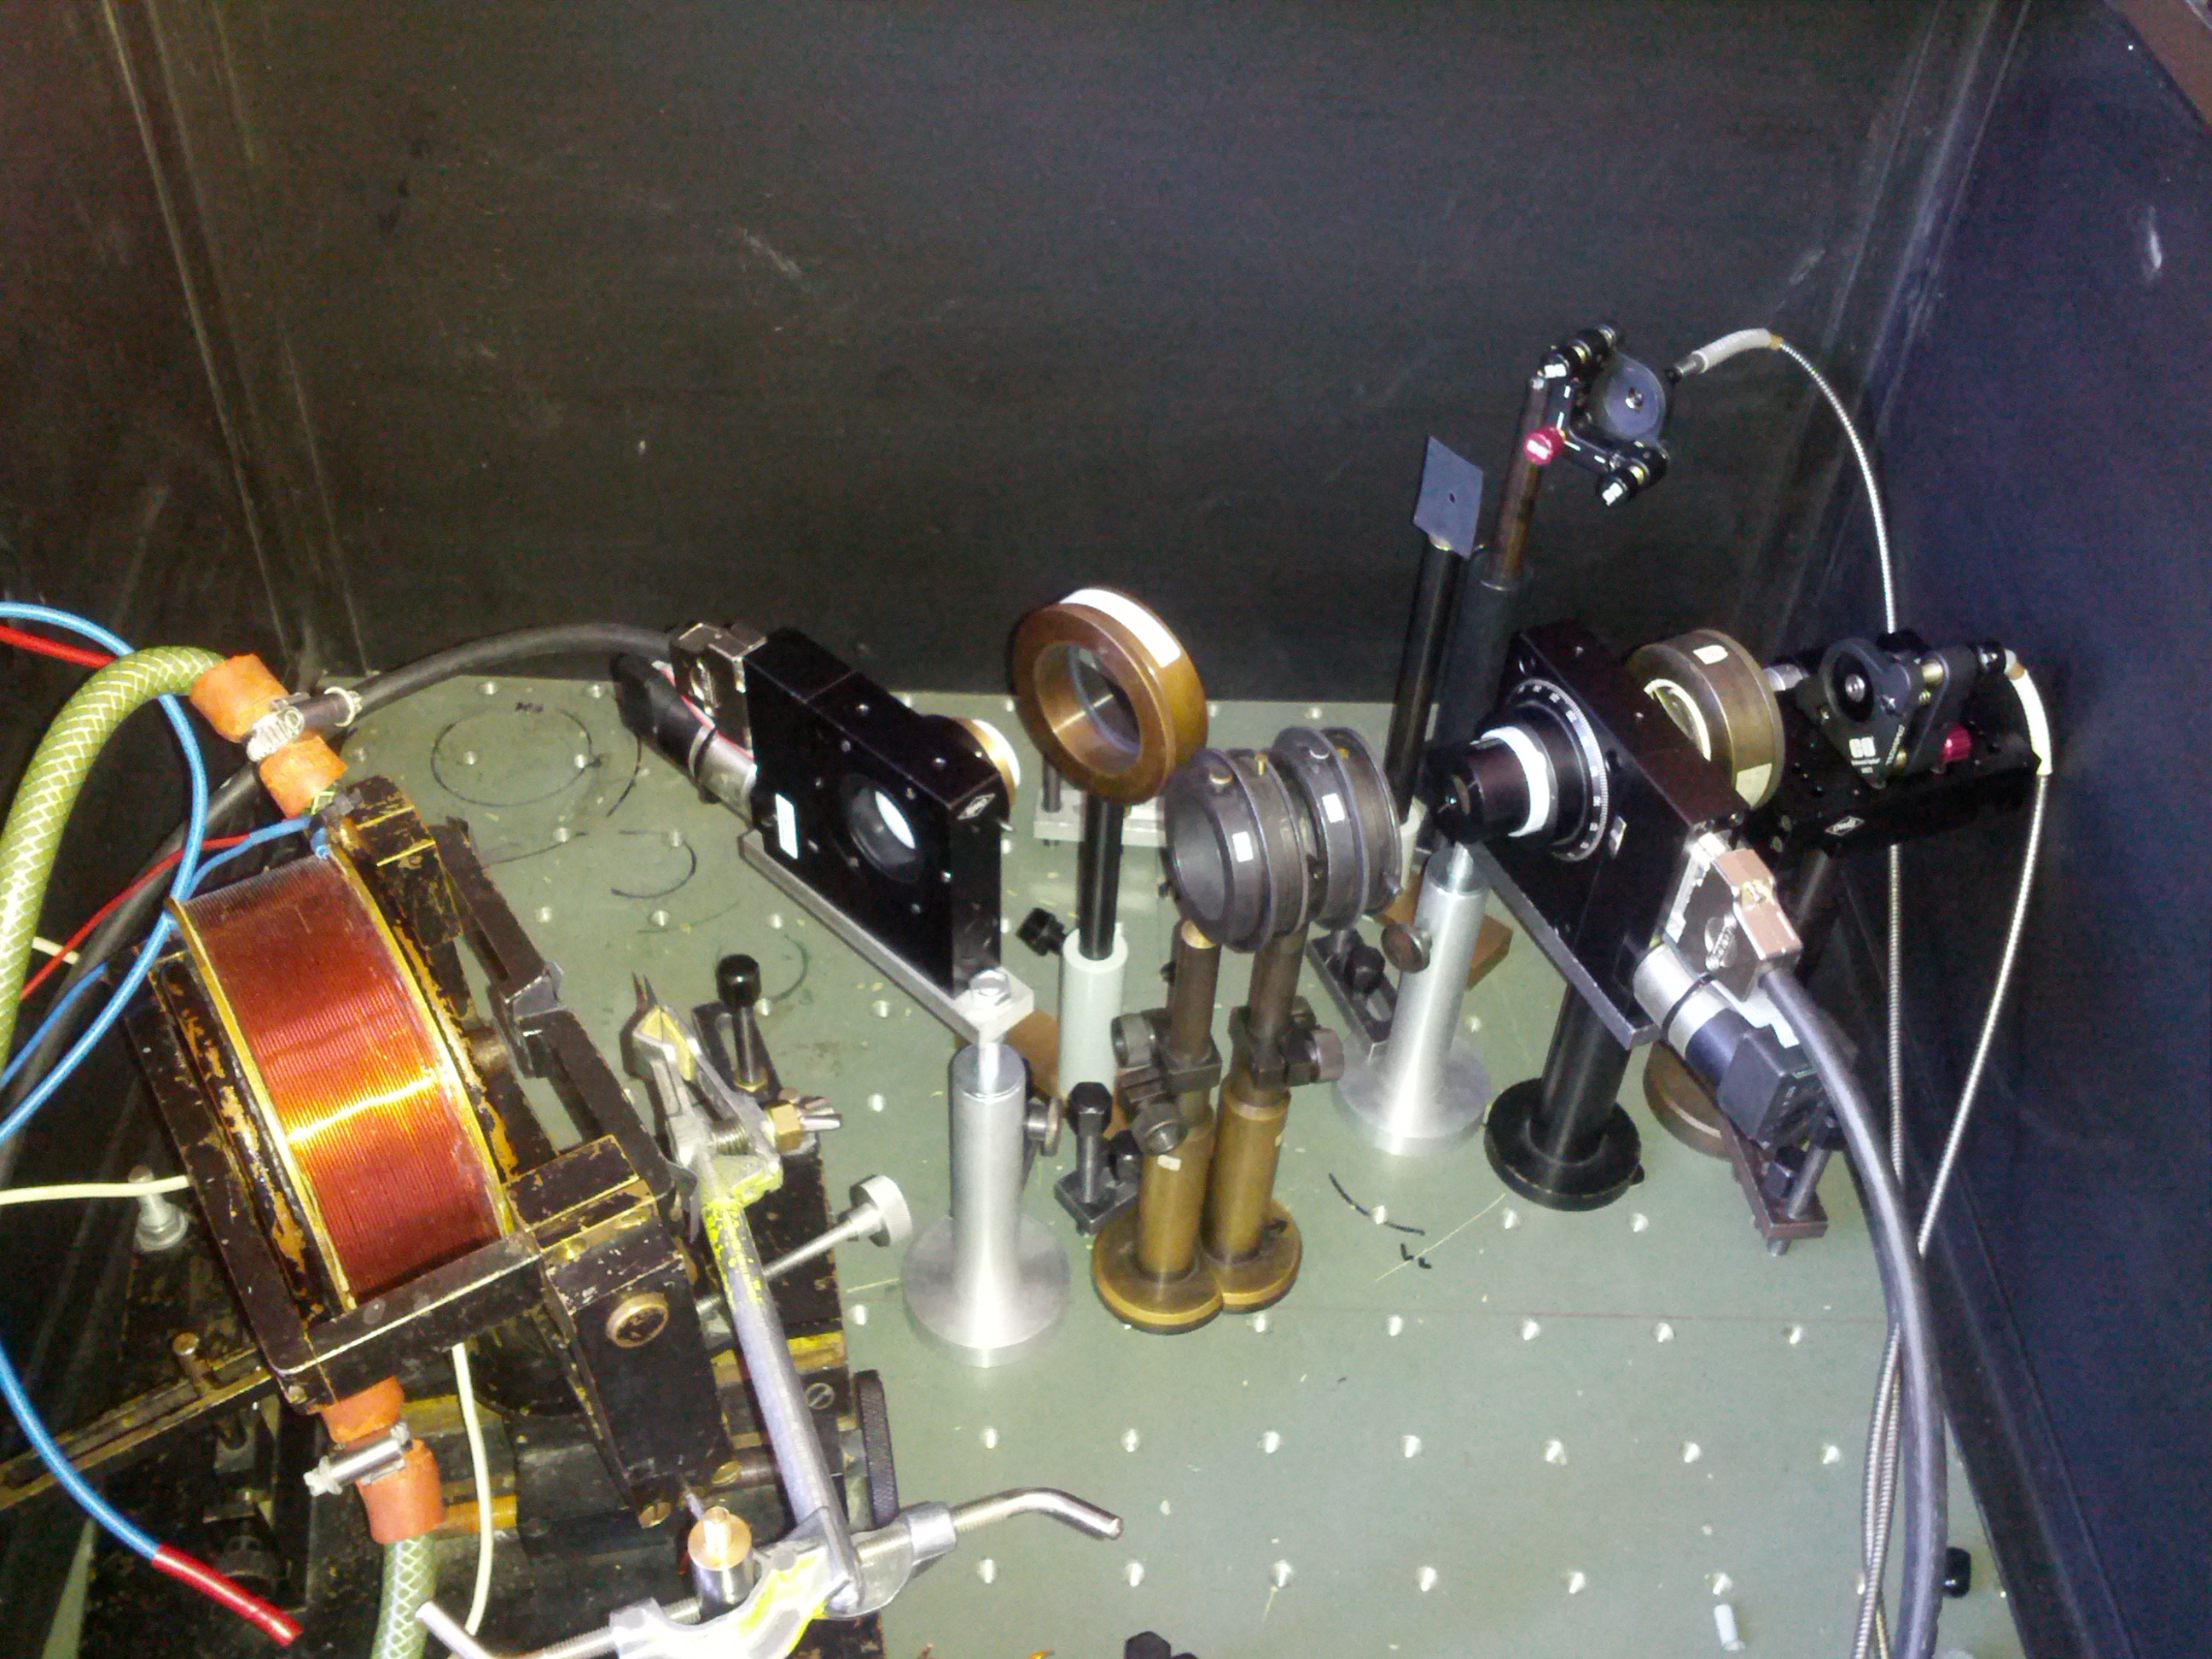
\includegraphics[width=5in]{img/TPEPhoto.eps}
\caption{Fotografie aparatury pro metodu skřížených polarizátorů}
\label{TPE photo}
\end{center}
\end{figure}

Jako zdroj světla používáme lampu typ DH-2000-BAL od Ocean Optics. Tato lampa obsahuje deuteriovou a halogenovou trubici. Obě najedou pokrývají spektrální rozsah od 215 nm do 2500 nm, což dalece přesahuje rozsah detektoru. Intenzita světla je téměř stejná v celém spektru, avšak část oblasti malých vlnových délek je ztracena především v optických vláken. Z toho důvodu vzniká v této oblasti výrazně větší spektrální šum, avšak dostatečná doba integrace signálu tuto vadu téměř zcela vyruší.

Polarizátory z CaF a křemene typu Rochon jsou umístěny do držáků s krokovými motorky.  Ty umožňují nastavení úhlu s přesností až $10^{-3}$ stupně. Jejich ovládání je zprostředkováno kontrolní jednotkou DC 500 od společnosti Owis. Ta umožňuje jejich manuální ovládání i kontrolu přes rozhraní GPIB.

V našem uspořádání vytváří magnet polární magnetické pole. Aby nedocházelo ke zahřívání vzorku, je celý magnet chlazený studenou vodou. Při proudu 2 A vytváří magnet pole okolo 0.4 T, které bylo dostatečné k nasycení měřených vzorků. %TODO Hysterzní smyška

K analýze světla používáme CCD spektrometr USB2000+ od Ocean Optics. Jeho schéma naleznete na obrázku (\ref{USB2000+ schema}), přičemž opis jednotlivých komponent naleznete v \cite{USB2000}. Rozsah spektrometru je přibližně od 200 do 900 nm s rozlišovací schopností 0.3 nm (FWHM). Komunikace se spektrometrem je zprostředkována přes rozhraní USB protokolem VISA. 

\begin{figure}
    \begin{center}
    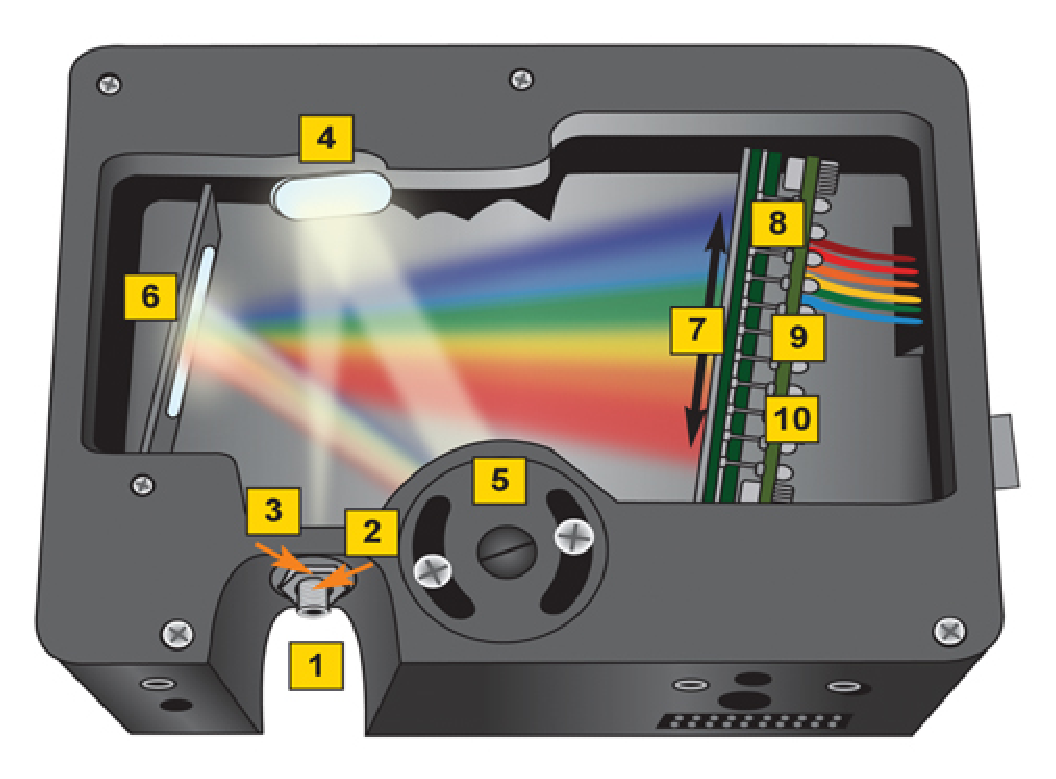
\includegraphics[width=5in]{img/usb4openbench.eps}
    \end{center}
    \caption{Schéma sektrometru USB2000+}
    \label{USB2000+ schema}
\end{figure}

\subsection{Průběh měření}
Samotné měření se dá rozdělit do dvou částí. První je nastavení aparatury a druhá samotné měření. Toto rozdělení respektuje i ovládací program.
\subsubsection{Nastavení aparatury}
Po upevnění vzorku je nejprve třeba navést světelný svazek do vlákna spektrometru. Ač je na jeho začátku sběrná čočka, je třeba velmi jemného nastavení za pomoci aretačních šroubů, protože natočení této čočky má velký vliv na měřenou intenzitu.

Následně je potřeba nastavit první polarizátor tak abychom získali p-polarizované světlo. Proto za něj umístíme sklíčko tak, aby úhel odrazu do detektoru odpovídal Brewsterově úhlu. Díky tomu pro nastavení polarizátoru na p-polarizaci detekujeme minimální intenzitu světla. To platí nezávisle na vlnové délce, proto je nejvhodnější vyhodnocovat pouze neiintenzivnější část spektra. Minimum nalezneme tak, že proskenujeme různé úhly natočení polarizátoru a následně zhustšujeme měření v oblasti minima, dokud nedosáhneme požadované přesnosti.

Druhý polarizátor je nutné pouze zkřížit, aby měřené závislosti byli co nejsymetričtější, což usnadňuje fitování. Toho docílíme podobně jako u prvního, protože se opět jedná o hledání minima signálu při nulovém magnetickém poli.

Aby nebylo nutné nastavovat aparaturu před každým měřením, jsou natočení polarizátoru uchovávány v externím souboru a při spuštění programu se použijí, pokud nastavování neproběhne. Díky tomu je kalibrace nutná pouze v případě zásahu do aparatury. 


\subsection{Měření}
Na začátku měření zadáme rozsah úhlu, které budeme měřit, krok, četnost měření spekter pro jednotlivé úhly a proud pro magnet. Tyto údaje mají velký vliv na úroveň šumu spektra a na dobu měření. Spektra při různých hodnotách jsou znázorněna na obrázcích (\ref{TPE1}) až (\ref{TPE3}) spektra při změnách těchto parametrů. Při našem nastavení stačí pro hrubý odhad spektra okolo 40 měření při četnosti 100. Takové měření trvá několik málo minut. Pokud však chceme minimální šum, měříme v rozahu od -40 do 40 stupňů s krokem 0.5 stupně a četnosti 500. Toto měření již trvá okolo 40 minut, ale jak je vidět na spektrech, výsledky jsou výrazně hladší.

Pro fitování předepsané závislosti (\ref{I2}) používáme Krameriovu metodu. Vzhledek k posunu nulové intenzity na detektoru je konečná fitovaná závislost
\begin{eqnarray}
I(\alpha)=a_1+a_2\sin^2(\alpha)+a_3\sin(2\alpha)
\end{eqnarray}
kde $a_1$ odpovídá zmíněnému posunu, $a_2$ je úměrné reflektivitě vzroku, ale vzhledem ke ztrátám na optických prvcích a v optickém vlákně nemá přílišný význam a z $a_3$ dopočteme za pomoci vztahu $\frac{a_3}{a_2}=(\theta_K\cos\delta+\epsilon_K\sin\delta)$ příslušný elisometrický koeficient, jak už bylo zmíněno výše. Ukázku naměřený závislosti pro $\lambda=520$ nm s nafitovanými křivkami naleznete na obrázku (\ref{TPE0}).

\begin{figure}
% GNUPLOT: LaTeX picture with Postscript
\begingroup
  \makeatletter
  \providecommand\color[2][]{%
    \GenericError{(gnuplot) \space\space\space\@spaces}{%
      Package color not loaded in conjunction with
      terminal option `colourtext'%
    }{See the gnuplot documentation for explanation.%
    }{Either use 'blacktext' in gnuplot or load the package
      color.sty in LaTeX.}%
    \renewcommand\color[2][]{}%
  }%
  \providecommand\includegraphics[2][]{%
    \GenericError{(gnuplot) \space\space\space\@spaces}{%
      Package graphicx or graphics not loaded%
    }{See the gnuplot documentation for explanation.%
    }{The gnuplot epslatex terminal needs graphicx.sty or graphics.sty.}%
    \renewcommand\includegraphics[2][]{}%
  }%
  \providecommand\rotatebox[2]{#2}%
  \@ifundefined{ifGPcolor}{%
    \newif\ifGPcolor
    \GPcolorfalse
  }{}%
  \@ifundefined{ifGPblacktext}{%
    \newif\ifGPblacktext
    \GPblacktexttrue
  }{}%
  % define a \g@addto@macro without @ in the name:
  \let\gplgaddtomacro\g@addto@macro
  % define empty templates for all commands taking text:
  \gdef\gplbacktext{}%
  \gdef\gplfronttext{}%
  \makeatother
  \ifGPblacktext
    % no textcolor at all
    \def\colorrgb#1{}%
    \def\colorgray#1{}%
  \else
    % gray or color?
    \ifGPcolor
      \def\colorrgb#1{\color[rgb]{#1}}%
      \def\colorgray#1{\color[gray]{#1}}%
      \expandafter\def\csname LTw\endcsname{\color{white}}%
      \expandafter\def\csname LTb\endcsname{\color{black}}%
      \expandafter\def\csname LTa\endcsname{\color{black}}%
      \expandafter\def\csname LT0\endcsname{\color[rgb]{1,0,0}}%
      \expandafter\def\csname LT1\endcsname{\color[rgb]{0,1,0}}%
      \expandafter\def\csname LT2\endcsname{\color[rgb]{0,0,1}}%
      \expandafter\def\csname LT3\endcsname{\color[rgb]{1,0,1}}%
      \expandafter\def\csname LT4\endcsname{\color[rgb]{0,1,1}}%
      \expandafter\def\csname LT5\endcsname{\color[rgb]{1,1,0}}%
      \expandafter\def\csname LT6\endcsname{\color[rgb]{0,0,0}}%
      \expandafter\def\csname LT7\endcsname{\color[rgb]{1,0.3,0}}%
      \expandafter\def\csname LT8\endcsname{\color[rgb]{0.5,0.5,0.5}}%
    \else
      % gray
      \def\colorrgb#1{\color{black}}%
      \def\colorgray#1{\color[gray]{#1}}%
      \expandafter\def\csname LTw\endcsname{\color{white}}%
      \expandafter\def\csname LTb\endcsname{\color{black}}%
      \expandafter\def\csname LTa\endcsname{\color{black}}%
      \expandafter\def\csname LT0\endcsname{\color{black}}%
      \expandafter\def\csname LT1\endcsname{\color{black}}%
      \expandafter\def\csname LT2\endcsname{\color{black}}%
      \expandafter\def\csname LT3\endcsname{\color{black}}%
      \expandafter\def\csname LT4\endcsname{\color{black}}%
      \expandafter\def\csname LT5\endcsname{\color{black}}%
      \expandafter\def\csname LT6\endcsname{\color{black}}%
      \expandafter\def\csname LT7\endcsname{\color{black}}%
      \expandafter\def\csname LT8\endcsname{\color{black}}%
    \fi
  \fi
  \setlength{\unitlength}{0.0500bp}%
  \begin{picture}(7200.00,5040.00)%
    \gplgaddtomacro\gplbacktext{%
      \csname LTb\endcsname%
      \put(1342,704){\makebox(0,0)[r]{\strut{} 0}}%
      \put(1342,1518){\makebox(0,0)[r]{\strut{} 5000}}%
      \put(1342,2332){\makebox(0,0)[r]{\strut{} 10000}}%
      \put(1342,3147){\makebox(0,0)[r]{\strut{} 15000}}%
      \put(1342,3961){\makebox(0,0)[r]{\strut{} 20000}}%
      \put(1342,4775){\makebox(0,0)[r]{\strut{} 25000}}%
      \put(1474,484){\makebox(0,0){\strut{}-40}}%
      \put(2148,484){\makebox(0,0){\strut{}-30}}%
      \put(2823,484){\makebox(0,0){\strut{}-20}}%
      \put(3497,484){\makebox(0,0){\strut{}-10}}%
      \put(4172,484){\makebox(0,0){\strut{} 0}}%
      \put(4846,484){\makebox(0,0){\strut{} 10}}%
      \put(5520,484){\makebox(0,0){\strut{} 20}}%
      \put(6195,484){\makebox(0,0){\strut{} 30}}%
      \put(6869,484){\makebox(0,0){\strut{} 40}}%
      \put(308,2739){\rotatebox{-270}{\makebox(0,0){\strut{}$I$}}}%
      \put(4171,154){\makebox(0,0){\strut{}$\alpha$/$^o$}}%
    }%
    \gplgaddtomacro\gplfronttext{%
      \csname LTb\endcsname%
      \put(5882,4602){\makebox(0,0)[r]{\strut{}$I=2$ A}}%
      \csname LTb\endcsname%
      \put(5882,4382){\makebox(0,0)[r]{\strut{}$I=-2$ A}}%
    }%
    \gplbacktext
    \put(0,0){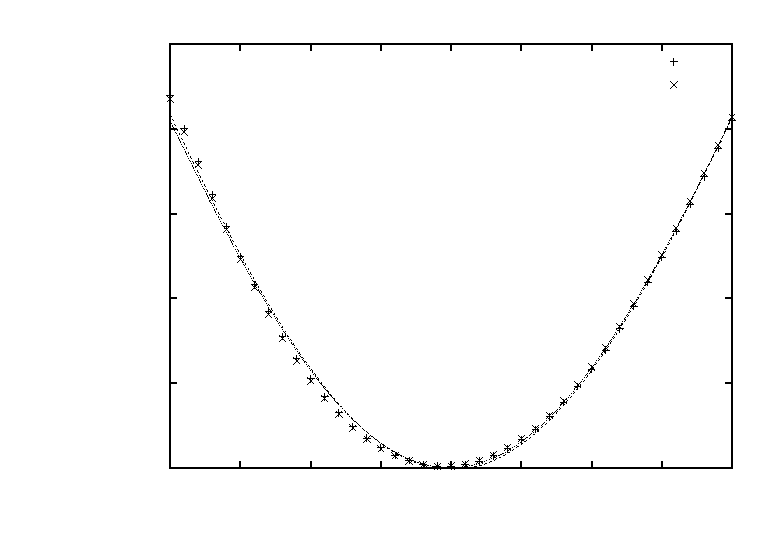
\includegraphics{TPE0}}%
    \gplfronttext
  \end{picture}%
\endgroup

\caption{Naměřená závislost intenzity na úhlu natočení polarizátoru pro $\lambda =520$ nm}
\label{TPE0}
\end{figure}

\begin{figure}
% GNUPLOT: LaTeX picture with Postscript
\begingroup
  \makeatletter
  \providecommand\color[2][]{%
    \GenericError{(gnuplot) \space\space\space\@spaces}{%
      Package color not loaded in conjunction with
      terminal option `colourtext'%
    }{See the gnuplot documentation for explanation.%
    }{Either use 'blacktext' in gnuplot or load the package
      color.sty in LaTeX.}%
    \renewcommand\color[2][]{}%
  }%
  \providecommand\includegraphics[2][]{%
    \GenericError{(gnuplot) \space\space\space\@spaces}{%
      Package graphicx or graphics not loaded%
    }{See the gnuplot documentation for explanation.%
    }{The gnuplot epslatex terminal needs graphicx.sty or graphics.sty.}%
    \renewcommand\includegraphics[2][]{}%
  }%
  \providecommand\rotatebox[2]{#2}%
  \@ifundefined{ifGPcolor}{%
    \newif\ifGPcolor
    \GPcolorfalse
  }{}%
  \@ifundefined{ifGPblacktext}{%
    \newif\ifGPblacktext
    \GPblacktexttrue
  }{}%
  % define a \g@addto@macro without @ in the name:
  \let\gplgaddtomacro\g@addto@macro
  % define empty templates for all commands taking text:
  \gdef\gplbacktext{}%
  \gdef\gplfronttext{}%
  \makeatother
  \ifGPblacktext
    % no textcolor at all
    \def\colorrgb#1{}%
    \def\colorgray#1{}%
  \else
    % gray or color?
    \ifGPcolor
      \def\colorrgb#1{\color[rgb]{#1}}%
      \def\colorgray#1{\color[gray]{#1}}%
      \expandafter\def\csname LTw\endcsname{\color{white}}%
      \expandafter\def\csname LTb\endcsname{\color{black}}%
      \expandafter\def\csname LTa\endcsname{\color{black}}%
      \expandafter\def\csname LT0\endcsname{\color[rgb]{1,0,0}}%
      \expandafter\def\csname LT1\endcsname{\color[rgb]{0,1,0}}%
      \expandafter\def\csname LT2\endcsname{\color[rgb]{0,0,1}}%
      \expandafter\def\csname LT3\endcsname{\color[rgb]{1,0,1}}%
      \expandafter\def\csname LT4\endcsname{\color[rgb]{0,1,1}}%
      \expandafter\def\csname LT5\endcsname{\color[rgb]{1,1,0}}%
      \expandafter\def\csname LT6\endcsname{\color[rgb]{0,0,0}}%
      \expandafter\def\csname LT7\endcsname{\color[rgb]{1,0.3,0}}%
      \expandafter\def\csname LT8\endcsname{\color[rgb]{0.5,0.5,0.5}}%
    \else
      % gray
      \def\colorrgb#1{\color{black}}%
      \def\colorgray#1{\color[gray]{#1}}%
      \expandafter\def\csname LTw\endcsname{\color{white}}%
      \expandafter\def\csname LTb\endcsname{\color{black}}%
      \expandafter\def\csname LTa\endcsname{\color{black}}%
      \expandafter\def\csname LT0\endcsname{\color{black}}%
      \expandafter\def\csname LT1\endcsname{\color{black}}%
      \expandafter\def\csname LT2\endcsname{\color{black}}%
      \expandafter\def\csname LT3\endcsname{\color{black}}%
      \expandafter\def\csname LT4\endcsname{\color{black}}%
      \expandafter\def\csname LT5\endcsname{\color{black}}%
      \expandafter\def\csname LT6\endcsname{\color{black}}%
      \expandafter\def\csname LT7\endcsname{\color{black}}%
      \expandafter\def\csname LT8\endcsname{\color{black}}%
    \fi
  \fi
  \setlength{\unitlength}{0.0500bp}%
  \begin{picture}(7200.00,5040.00)%
    \gplgaddtomacro\gplbacktext{%
      \csname LTb\endcsname%
      \put(1342,704){\makebox(0,0)[r]{\strut{}-0.02}}%
      \put(1342,1213){\makebox(0,0)[r]{\strut{}-0.015}}%
      \put(1342,1722){\makebox(0,0)[r]{\strut{}-0.01}}%
      \put(1342,2231){\makebox(0,0)[r]{\strut{}-0.005}}%
      \put(1342,2740){\makebox(0,0)[r]{\strut{} 0}}%
      \put(1342,3248){\makebox(0,0)[r]{\strut{} 0.005}}%
      \put(1342,3757){\makebox(0,0)[r]{\strut{} 0.01}}%
      \put(1342,4266){\makebox(0,0)[r]{\strut{} 0.015}}%
      \put(1342,4775){\makebox(0,0)[r]{\strut{} 0.02}}%
      \put(1731,484){\makebox(0,0){\strut{} 300}}%
      \put(2587,484){\makebox(0,0){\strut{} 400}}%
      \put(3444,484){\makebox(0,0){\strut{} 500}}%
      \put(4300,484){\makebox(0,0){\strut{} 600}}%
      \put(5156,484){\makebox(0,0){\strut{} 700}}%
      \put(6013,484){\makebox(0,0){\strut{} 800}}%
      \put(6869,484){\makebox(0,0){\strut{} 900}}%
      \put(308,2739){\rotatebox{-270}{\makebox(0,0){\strut{}$\theta_K$}}}%
      \put(4171,154){\makebox(0,0){\strut{}$\lambda$/nm}}%
    }%
    \gplgaddtomacro\gplfronttext{%
      \csname LTb\endcsname%
      \put(5882,4602){\makebox(0,0)[r]{\strut{}80 měření}}%
      \csname LTb\endcsname%
      \put(5882,4382){\makebox(0,0)[r]{\strut{}320 měření}}%
    }%
    \gplbacktext
    \put(0,0){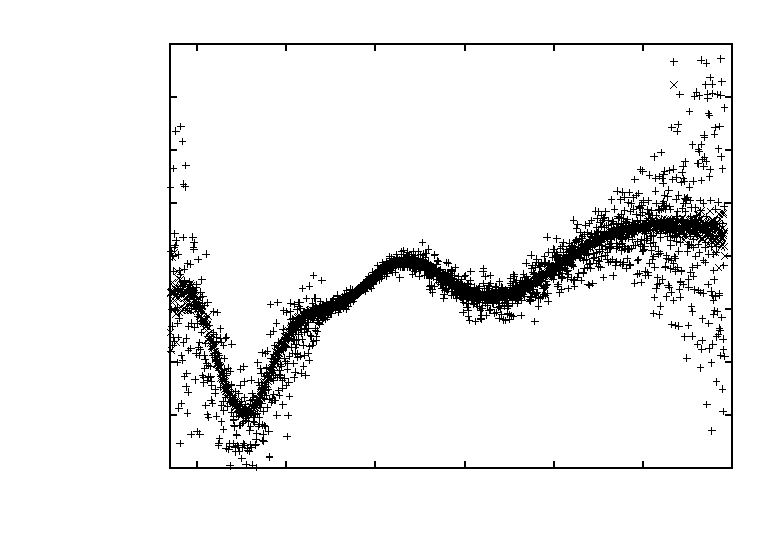
\includegraphics{TPE1}}%
    \gplfronttext
  \end{picture}%
\endgroup

\caption{Naměřené spektrum v pro různé množství měřených úhlů.}
\label{TPE1}
\end{figure}

\begin{figure}
% GNUPLOT: LaTeX picture with Postscript
\begingroup
  \makeatletter
  \providecommand\color[2][]{%
    \GenericError{(gnuplot) \space\space\space\@spaces}{%
      Package color not loaded in conjunction with
      terminal option `colourtext'%
    }{See the gnuplot documentation for explanation.%
    }{Either use 'blacktext' in gnuplot or load the package
      color.sty in LaTeX.}%
    \renewcommand\color[2][]{}%
  }%
  \providecommand\includegraphics[2][]{%
    \GenericError{(gnuplot) \space\space\space\@spaces}{%
      Package graphicx or graphics not loaded%
    }{See the gnuplot documentation for explanation.%
    }{The gnuplot epslatex terminal needs graphicx.sty or graphics.sty.}%
    \renewcommand\includegraphics[2][]{}%
  }%
  \providecommand\rotatebox[2]{#2}%
  \@ifundefined{ifGPcolor}{%
    \newif\ifGPcolor
    \GPcolorfalse
  }{}%
  \@ifundefined{ifGPblacktext}{%
    \newif\ifGPblacktext
    \GPblacktexttrue
  }{}%
  % define a \g@addto@macro without @ in the name:
  \let\gplgaddtomacro\g@addto@macro
  % define empty templates for all commands taking text:
  \gdef\gplbacktext{}%
  \gdef\gplfronttext{}%
  \makeatother
  \ifGPblacktext
    % no textcolor at all
    \def\colorrgb#1{}%
    \def\colorgray#1{}%
  \else
    % gray or color?
    \ifGPcolor
      \def\colorrgb#1{\color[rgb]{#1}}%
      \def\colorgray#1{\color[gray]{#1}}%
      \expandafter\def\csname LTw\endcsname{\color{white}}%
      \expandafter\def\csname LTb\endcsname{\color{black}}%
      \expandafter\def\csname LTa\endcsname{\color{black}}%
      \expandafter\def\csname LT0\endcsname{\color[rgb]{1,0,0}}%
      \expandafter\def\csname LT1\endcsname{\color[rgb]{0,1,0}}%
      \expandafter\def\csname LT2\endcsname{\color[rgb]{0,0,1}}%
      \expandafter\def\csname LT3\endcsname{\color[rgb]{1,0,1}}%
      \expandafter\def\csname LT4\endcsname{\color[rgb]{0,1,1}}%
      \expandafter\def\csname LT5\endcsname{\color[rgb]{1,1,0}}%
      \expandafter\def\csname LT6\endcsname{\color[rgb]{0,0,0}}%
      \expandafter\def\csname LT7\endcsname{\color[rgb]{1,0.3,0}}%
      \expandafter\def\csname LT8\endcsname{\color[rgb]{0.5,0.5,0.5}}%
    \else
      % gray
      \def\colorrgb#1{\color{black}}%
      \def\colorgray#1{\color[gray]{#1}}%
      \expandafter\def\csname LTw\endcsname{\color{white}}%
      \expandafter\def\csname LTb\endcsname{\color{black}}%
      \expandafter\def\csname LTa\endcsname{\color{black}}%
      \expandafter\def\csname LT0\endcsname{\color{black}}%
      \expandafter\def\csname LT1\endcsname{\color{black}}%
      \expandafter\def\csname LT2\endcsname{\color{black}}%
      \expandafter\def\csname LT3\endcsname{\color{black}}%
      \expandafter\def\csname LT4\endcsname{\color{black}}%
      \expandafter\def\csname LT5\endcsname{\color{black}}%
      \expandafter\def\csname LT6\endcsname{\color{black}}%
      \expandafter\def\csname LT7\endcsname{\color{black}}%
      \expandafter\def\csname LT8\endcsname{\color{black}}%
    \fi
  \fi
  \setlength{\unitlength}{0.0500bp}%
  \begin{picture}(7200.00,5040.00)%
    \gplgaddtomacro\gplbacktext{%
      \csname LTb\endcsname%
      \put(1342,704){\makebox(0,0)[r]{\strut{}-0.02}}%
      \put(1342,1213){\makebox(0,0)[r]{\strut{}-0.015}}%
      \put(1342,1722){\makebox(0,0)[r]{\strut{}-0.01}}%
      \put(1342,2231){\makebox(0,0)[r]{\strut{}-0.005}}%
      \put(1342,2740){\makebox(0,0)[r]{\strut{} 0}}%
      \put(1342,3248){\makebox(0,0)[r]{\strut{} 0.005}}%
      \put(1342,3757){\makebox(0,0)[r]{\strut{} 0.01}}%
      \put(1342,4266){\makebox(0,0)[r]{\strut{} 0.015}}%
      \put(1342,4775){\makebox(0,0)[r]{\strut{} 0.02}}%
      \put(1624,484){\makebox(0,0){\strut{} 1.5}}%
      \put(2373,484){\makebox(0,0){\strut{} 2}}%
      \put(3122,484){\makebox(0,0){\strut{} 2.5}}%
      \put(3872,484){\makebox(0,0){\strut{} 3}}%
      \put(4621,484){\makebox(0,0){\strut{} 3.5}}%
      \put(5370,484){\makebox(0,0){\strut{} 4}}%
      \put(6120,484){\makebox(0,0){\strut{} 4.5}}%
      \put(6869,484){\makebox(0,0){\strut{} 5}}%
      \put(308,2739){\rotatebox{-270}{\makebox(0,0){\strut{}$\theta_K$}}}%
      \put(4171,154){\makebox(0,0){\strut{}$E$/eV}}%
    }%
    \gplgaddtomacro\gplfronttext{%
      \csname LTb\endcsname%
      \put(5882,4602){\makebox(0,0)[r]{\strut{}1s}}%
      \csname LTb\endcsname%
      \put(5882,4382){\makebox(0,0)[r]{\strut{}5s}}%
    }%
    \gplbacktext
    \put(0,0){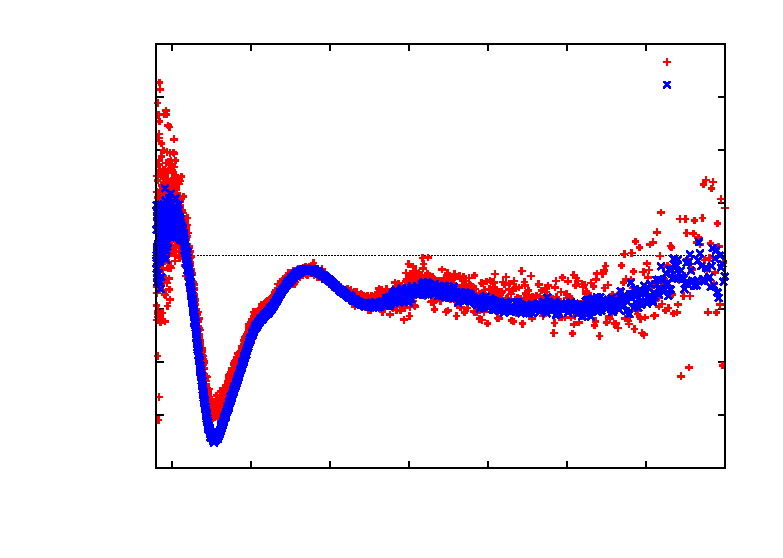
\includegraphics{TPE2}}%
    \gplfronttext
  \end{picture}%
\endgroup

\caption{Naměřené spektrum v pro různé integrační doby spektra.}
\label{TPE2}
\end{figure}

\begin{figure}
% GNUPLOT: LaTeX picture with Postscript
\begingroup
  \makeatletter
  \providecommand\color[2][]{%
    \GenericError{(gnuplot) \space\space\space\@spaces}{%
      Package color not loaded in conjunction with
      terminal option `colourtext'%
    }{See the gnuplot documentation for explanation.%
    }{Either use 'blacktext' in gnuplot or load the package
      color.sty in LaTeX.}%
    \renewcommand\color[2][]{}%
  }%
  \providecommand\includegraphics[2][]{%
    \GenericError{(gnuplot) \space\space\space\@spaces}{%
      Package graphicx or graphics not loaded%
    }{See the gnuplot documentation for explanation.%
    }{The gnuplot epslatex terminal needs graphicx.sty or graphics.sty.}%
    \renewcommand\includegraphics[2][]{}%
  }%
  \providecommand\rotatebox[2]{#2}%
  \@ifundefined{ifGPcolor}{%
    \newif\ifGPcolor
    \GPcolorfalse
  }{}%
  \@ifundefined{ifGPblacktext}{%
    \newif\ifGPblacktext
    \GPblacktexttrue
  }{}%
  % define a \g@addto@macro without @ in the name:
  \let\gplgaddtomacro\g@addto@macro
  % define empty templates for all commands taking text:
  \gdef\gplbacktext{}%
  \gdef\gplfronttext{}%
  \makeatother
  \ifGPblacktext
    % no textcolor at all
    \def\colorrgb#1{}%
    \def\colorgray#1{}%
  \else
    % gray or color?
    \ifGPcolor
      \def\colorrgb#1{\color[rgb]{#1}}%
      \def\colorgray#1{\color[gray]{#1}}%
      \expandafter\def\csname LTw\endcsname{\color{white}}%
      \expandafter\def\csname LTb\endcsname{\color{black}}%
      \expandafter\def\csname LTa\endcsname{\color{black}}%
      \expandafter\def\csname LT0\endcsname{\color[rgb]{1,0,0}}%
      \expandafter\def\csname LT1\endcsname{\color[rgb]{0,1,0}}%
      \expandafter\def\csname LT2\endcsname{\color[rgb]{0,0,1}}%
      \expandafter\def\csname LT3\endcsname{\color[rgb]{1,0,1}}%
      \expandafter\def\csname LT4\endcsname{\color[rgb]{0,1,1}}%
      \expandafter\def\csname LT5\endcsname{\color[rgb]{1,1,0}}%
      \expandafter\def\csname LT6\endcsname{\color[rgb]{0,0,0}}%
      \expandafter\def\csname LT7\endcsname{\color[rgb]{1,0.3,0}}%
      \expandafter\def\csname LT8\endcsname{\color[rgb]{0.5,0.5,0.5}}%
    \else
      % gray
      \def\colorrgb#1{\color{black}}%
      \def\colorgray#1{\color[gray]{#1}}%
      \expandafter\def\csname LTw\endcsname{\color{white}}%
      \expandafter\def\csname LTb\endcsname{\color{black}}%
      \expandafter\def\csname LTa\endcsname{\color{black}}%
      \expandafter\def\csname LT0\endcsname{\color{black}}%
      \expandafter\def\csname LT1\endcsname{\color{black}}%
      \expandafter\def\csname LT2\endcsname{\color{black}}%
      \expandafter\def\csname LT3\endcsname{\color{black}}%
      \expandafter\def\csname LT4\endcsname{\color{black}}%
      \expandafter\def\csname LT5\endcsname{\color{black}}%
      \expandafter\def\csname LT6\endcsname{\color{black}}%
      \expandafter\def\csname LT7\endcsname{\color{black}}%
      \expandafter\def\csname LT8\endcsname{\color{black}}%
    \fi
  \fi
  \setlength{\unitlength}{0.0500bp}%
  \begin{picture}(7200.00,5040.00)%
    \gplgaddtomacro\gplbacktext{%
      \csname LTb\endcsname%
      \put(1342,704){\makebox(0,0)[r]{\strut{}-0.02}}%
      \put(1342,1213){\makebox(0,0)[r]{\strut{}-0.015}}%
      \put(1342,1722){\makebox(0,0)[r]{\strut{}-0.01}}%
      \put(1342,2231){\makebox(0,0)[r]{\strut{}-0.005}}%
      \put(1342,2740){\makebox(0,0)[r]{\strut{} 0}}%
      \put(1342,3248){\makebox(0,0)[r]{\strut{} 0.005}}%
      \put(1342,3757){\makebox(0,0)[r]{\strut{} 0.01}}%
      \put(1342,4266){\makebox(0,0)[r]{\strut{} 0.015}}%
      \put(1342,4775){\makebox(0,0)[r]{\strut{} 0.02}}%
      \put(1624,484){\makebox(0,0){\strut{} 1.5}}%
      \put(2373,484){\makebox(0,0){\strut{} 2}}%
      \put(3122,484){\makebox(0,0){\strut{} 2.5}}%
      \put(3872,484){\makebox(0,0){\strut{} 3}}%
      \put(4621,484){\makebox(0,0){\strut{} 3.5}}%
      \put(5370,484){\makebox(0,0){\strut{} 4}}%
      \put(6120,484){\makebox(0,0){\strut{} 4.5}}%
      \put(6869,484){\makebox(0,0){\strut{} 5}}%
      \put(308,2739){\rotatebox{-270}{\makebox(0,0){\strut{}$\theta_K$}}}%
      \put(4171,154){\makebox(0,0){\strut{}$E$/eV}}%
    }%
    \gplgaddtomacro\gplfronttext{%
      \csname LTb\endcsname%
      \put(3322,4602){\makebox(0,0)[r]{\strut{}40 mereni 1s}}%
      \csname LTb\endcsname%
      \put(3322,4382){\makebox(0,0)[r]{\strut{}120 mereni 2s}}%
      \csname LTb\endcsname%
      \put(3322,4162){\makebox(0,0)[r]{\strut{}240 mereni 5s}}%
    }%
    \gplbacktext
    \put(0,0){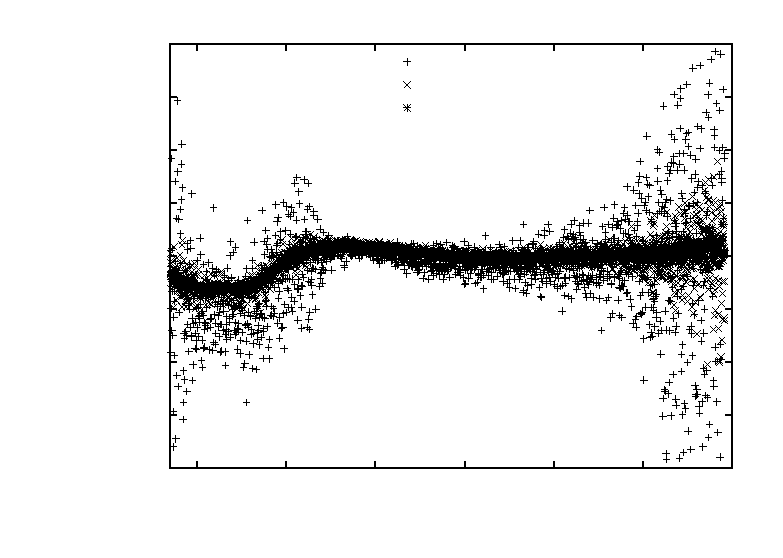
\includegraphics{img/TPE3}}%
    \gplfronttext
  \end{picture}%
\endgroup

\caption{Naměřené spektrum v pro různé množství měření a integrační doby spektra.}
\label{TPE3}
\end{figure}


\section{Modulační metoda}
Druhá aparatura, kterou používáme je na obrázku (\ref{Schema modul}). Sestává z monochromátoru, polarizátoru, Faradayovy nulovací cely, Faradayovy modulační cely, fázové destičky, vzorku v magnetickém poli, analyzátoru zkříženým s polarizátorem a fotonásobiče s detektorem. 
Faradayova cela, jak již bylo zmíněno v úvodu, stáčí rovinu polarizovaného světla v závislosti na velikosti magnetického pole. To je řízeno proudem vcívkce, která je navinutá kolem skleněného válce, kterým prochází světlo.

Jonesův vektor světla na konci aparatury získáme anoalogicky jako v předešlém případě.
\begin{eqnarray}
J=\begin{bmatrix}0&0\\0&1\end{bmatrix}
\begin{bmatrix}r_{ss}&r_{sp}\\r_{ps}& r_{pp}\end{bmatrix}
\begin{bmatrix}e^{i\frac{\delta}{2}}&0\\0&e^{-i\frac{\delta}{2}}\end{bmatrix}
\begin{bmatrix}\cos(\beta_0\sin\omega_mt) & -\sin(\beta_0\sin\omega_mt) \\ \sin(\beta_0\sin\omega_mt)&\cos(\beta_0\sin\omega_mt)\end{bmatrix}
\begin{bmatrix}\cos\eta&-\sin\eta\\\sin\eta&\cos\eta\end{bmatrix} \\
\begin{bmatrix}\sin\alpha\\\cos\alpha\end{bmatrix} \\
=\begin{bmatrix}0\\\cos\eta(r_{ps}e^{i\frac{\delta}{2}}\cos\tau+r_{pp}e^{-i\frac{\delta}{2}}\sin\tau)& -\sin\eta(r_{ps}e^{i\frac{\delta}{2}}\sin\tau-t_{pp}e^{-i\frac{\delta}{2}}\cos\tau)\end{bmatrix};\\ \tau = \beta_0\sin\omega_mt
\end{eqnarray}
Po další úpravách, které jsou podrobněji rozebrány například v \cite{Nyvlt} získáme vztah pro intenzitu
\begin{eqnarray}
I\approx\frac{1}{2}\left[|r_{ps}|^2+|r_{pp}|^2(\eta+\tau)+(r_{ps}r^*_{pp}e^{i\delta})^2+r^*_{ps}r_{pp}e^{-i\delta})(\eta+\tau)\right]
\end{eqnarray}
a oscilující komponenta při $\omega_m$ je
\begin{eqnarray}
I_{\omega_m}\approx|r_{pp}|^2\left[\eta+\mbox{Re}\left(\frac{r_{ps}}{r_{pp}}e^{i\delta}\right)\right]\tau
\end{eqnarray}
V našem případě používáme synchronní detekci. Velikost Kerrova jevu určujeme z oscilující složky úměrné $\omega_m$.

\begin{figure}
    \begin{center}
    \includegraphics[width=5in]{img/MO_setup.eps}
    \end{center}
    \caption{Schéma modulační metody}
    \label{Schema modul}
\end{figure}

\section{Zařízení}
Nová aparatrura obsahuje monochromátor TRIAX 550. Jedná se o mřížkový monochromátor s možností volby z různých mřížek. V našem případě máme na výběr 600, 900 a 1200 vrypů na mm. Parametry těchto mřížek jsou uvedeny v tabulce (\ref{TTriax}). Tento monochromátor lze ovládat za pomoci rozhraní GPIB. 
\begin{table}
$$
\begin{array}{|c|c|c|}
\hline
\mbox{grating} [g/mm]&  \mbox{Disperze} [nm/mm]&    \mbox{Spektrální rozsah} [nm] \\ \hline
600&    2.83&   0 - 3000 \\ \hline
900&    1.84&   0 - 2000 \\ \hline
1200&   1.34&   0 - 1500 \\ \hline
\end{array}
$$
\caption{Parametry mřížek monochromátoru}
\label{TTriax}
\end{table}

K Určení velikosti signálu na fotonásobiči používáme mulimetr Keithley 2001. V našem případě v měříme napětí na rozsahu 1 V při kterém má přesnost $\pm(0.0045\%+0.0008)$V. Možnost automatického rozsahu nepoužíváme, protože při přepnutí rozsahu dochází ke skokům napětí. Komunikace je opět zprostředkována rozhraním GPIB.

Jako zroj elektrického proudu pro magnet používáme zdroj stejnosměrbého proudu Kepco BOP. Standartně do magnetu pouštíme $\pm 2.5$A. Při této hodnotě je chyba proudu 0.1 mA. Při přepólování magnetu je nutné měnit proud postupně, jinak by mohlo dojít ke zkratu na zdroji. V našem případě používáme krok 0.05 A za 0.1 sekundy.

\section{Ovládací program Kerr2}
V rámci náplně této práce byl zcela přeprogramován ovládaví program kvůli novým komponentám.

\subsection{Nastavení experimentu}
Tento program má několik funkcí, které usnadňují nastavení experimetnu. Konkrétně umožňuje manuální kontrolu magnetu a monochromátoru s tím, že má přednastavených několik užitečných nastavení pro nastavování experimentu.

\subsection{Měření spektra}
Program umožňuje proměření spektra ve zvoleném rozahu s libovolným krokem. Dále umožňuje nastavení tolerance chyby měření, čekací doby po přepólování magnetu, počet měření jednotlivé vlnové délky a kalibračních koeficientů pro výpočet energie signálu. Po zahájení měření program nejprve nastaví na monochromátoru měřenou vlnovou délku a zapne proud do magnetu. Proud je přidáván postupně kvůli možnému zkratu na zroji při rychlém přepólování. Každé spektrum se měří opakovaně dle zadání uživatele, přičemž v celém prlběhu měření je kontrolováno, zda nebyl překročen rozsah. V takovém případě se měření pozastaví, aby umožnilo manuální otočení polarizátoru a měření pokračuje znovu od poslední vlnové délky. Měření stejně probíhá i pro opačnou magnetizaci, přičemž program umožňuje zadání počtu otáček potřebných pro navrácení do rozsahu po změně polarizace. Nakonec je pro danou vlnovou délku provedeno třetí měření s původní magnetizací a je zkontrolována odchylka od prvního měření. V případě příliš velké odchylky se měření opakuje. Po skončení měření jsou data uložena do expterního souboru spolu se všemi parametry měření.

\subsection{Hysterzní smyčky}
Program dále umožňuje měření hysterzních smyček a to dvěma způsoby. První postupně proměří při zadané vlnové délce ekvidistantě různé hodnoty proudu od I po -I a zpět. Druhá metoda, tzv. four loop, spočívá v postupném proměření hodnot vzdálených o $\Delta$I od hodnoty proudu I resp -I, přičemž tato vzálenost roste se zadaným krokem. V průběhu měření je postupně vykreslován graf.

\chapter{Dosažené výsledky}
V této kapitole je rozebráno měření konkrétních vzorků, interpretace spekter a porovníní výsledů obou užitých metod. V obou případech 
bylo  měřeno v polární geometrii, přičemž dopad na vzrorek byl téměř kolmý. Magnetické pole generované magnetem bylo u modulační metody 1.2 T. Magnet 
použitý při metodě zkřížených polarizátorů generoval pole pouze 0.4 T.

\section{Ultratenké vrstvy La$_{2/3}$Sr$_{1/3}$MnO$_3$}
První sada zkoumaných vzorků jsou tenké vrstvy La$_{2/3}$Sr$_{1/3}$MnO$_3$ (LSMO). Tento materiál je zkoumán především kvůli jeho potenciálnímu použití v oblasti spintroniky. 
Ta vyžaduje, aby materiál měl různou vodivost pro různě spiny elektronů. Další důležitý požadavek je jejich Curieova teplota alespoň nad pokojovou teplotou, z důvodu 
použitelnosti v zařízeních pracujících právě při pokojové teplotě.

Tyto vzorky byly vyrobeny metodou pulsní laserové depozice (PLD). Tato metoda umožňuje vytváření tenkých filmů o tloušťkách menších než 50 nm. Ve zkratce metoda funguje na principu kondenzace plazmy odpařované za pomoci krátkých laserových pulsů. 
Zkoumané vzorky byly připraveny na substrátu SrTiO$_3$ (STO) s krystalografickou orientací (1 0 0) 
a mřížkovou konstantou $a_{STO}=3.905$~\AA. Mřížková konstanta LSMO je $a_{LSMO}=3.889$~\AA, důsledkem čehož dochází k vzniku pnutí v tenké vrtvě, což má za následek slabší feromagnetické vlastnosti. 
Tloušťky zkoumaných vzorků byly 23,1 nm (PLD 186) a 80,8 nm (PLD202). 

Výsledky měření těchto vzorků jsou na obrázcích \ref{sPLD186} a \ref{sPLD202}.
Na spektru PLD186 je vidět, že modulační metoda 
dává pro energie nad 4.3 eV nepřesné výsledky. V této oblasti je vidět pokles obou ekeftů k nule, 
který je způsoben postupnou ztrátou signálu na detektoru. Tu má na vině 
snížení účinnosti fotonásobiče, která by mohla být odstraněna například použitím fotonásobiče s obálkou z křemenného skla, které má výrazně lepší propustnost v UV.
Ještě výrazněji se tento ekeft projevil při měření vzorků Heuslerových slitin uvedených níže.

Dále je znatelný energetický posun celého spekra. To je následek horšího spektrálního rozlišení monochromátoru v modulační metodě. 
K tomu se ještě projevuje chybovost krokového motorku monochromátoru, který 
způsobuje další nepřesnost v určení vlnové délky světla.

Až na výše uvedené vady je vidět velmi dobrá shoda spekter obou metod. Díky tomu můžeme říct, že metoda zkřížených polarizátorů má stejně, jako modulční metoda, velmi 
vysokou citlivost i přesnost.

Ze vztahu (\ref{teor kerr}) můžme určit teoretické spektrum těchto vzorků. Hodnoty pro LSMO byli určeny s pomocí materiálových parametrů na 35 nm tenké vrstvě, která 
se již dá považovat za téměř objemový materiál. \cite{PLD}  Parametry STO pak byly získány za pomoci spektroskopické elipsometrie. Výsledné porovnání 
teoretických hodnot s výsledky metody zkřížených polarizátorů obou 
vzorků je zobrazeno na obrázcích \ref{sPLD186t} a \ref{sPLD202t}. Vidíme, že pro PLD186 jsme, až na malé odchylky v amplitudě získali poměrně dobrou schodu. 
Tento rozdíl amplitud může být dán tím, že materiálové konstanty byly určeny za jiné teploty. Díky shodě s teorií můžeme říct, že vzorek PLD186 má podobné magnetooptické vlastnosti jako objemové LSMO. 
U vzorku PLD202 již vidíme, že ke shodě nedošlo. Z toho vyplývá, že muselo dojít ke změně krystalografické struktury, která vedla ke změně magnetooptických vlastností.

\begin{figure}
% GNUPLOT: LaTeX picture with Postscript
\begingroup
  \makeatletter
  \providecommand\color[2][]{%
    \GenericError{(gnuplot) \space\space\space\@spaces}{%
      Package color not loaded in conjunction with
      terminal option `colourtext'%
    }{See the gnuplot documentation for explanation.%
    }{Either use 'blacktext' in gnuplot or load the package
      color.sty in LaTeX.}%
    \renewcommand\color[2][]{}%
  }%
  \providecommand\includegraphics[2][]{%
    \GenericError{(gnuplot) \space\space\space\@spaces}{%
      Package graphicx or graphics not loaded%
    }{See the gnuplot documentation for explanation.%
    }{The gnuplot epslatex terminal needs graphicx.sty or graphics.sty.}%
    \renewcommand\includegraphics[2][]{}%
  }%
  \providecommand\rotatebox[2]{#2}%
  \@ifundefined{ifGPcolor}{%
    \newif\ifGPcolor
    \GPcolorfalse
  }{}%
  \@ifundefined{ifGPblacktext}{%
    \newif\ifGPblacktext
    \GPblacktexttrue
  }{}%
  % define a \g@addto@macro without @ in the name:
  \let\gplgaddtomacro\g@addto@macro
  % define empty templates for all commands taking text:
  \gdef\gplbacktext{}%
  \gdef\gplfronttext{}%
  \makeatother
  \ifGPblacktext
    % no textcolor at all
    \def\colorrgb#1{}%
    \def\colorgray#1{}%
  \else
    % gray or color?
    \ifGPcolor
      \def\colorrgb#1{\color[rgb]{#1}}%
      \def\colorgray#1{\color[gray]{#1}}%
      \expandafter\def\csname LTw\endcsname{\color{white}}%
      \expandafter\def\csname LTb\endcsname{\color{black}}%
      \expandafter\def\csname LTa\endcsname{\color{black}}%
      \expandafter\def\csname LT0\endcsname{\color[rgb]{1,0,0}}%
      \expandafter\def\csname LT1\endcsname{\color[rgb]{0,1,0}}%
      \expandafter\def\csname LT2\endcsname{\color[rgb]{0,0,1}}%
      \expandafter\def\csname LT3\endcsname{\color[rgb]{1,0,1}}%
      \expandafter\def\csname LT4\endcsname{\color[rgb]{0,1,1}}%
      \expandafter\def\csname LT5\endcsname{\color[rgb]{1,1,0}}%
      \expandafter\def\csname LT6\endcsname{\color[rgb]{0,0,0}}%
      \expandafter\def\csname LT7\endcsname{\color[rgb]{1,0.3,0}}%
      \expandafter\def\csname LT8\endcsname{\color[rgb]{0.5,0.5,0.5}}%
    \else
      % gray
      \def\colorrgb#1{\color{black}}%
      \def\colorgray#1{\color[gray]{#1}}%
      \expandafter\def\csname LTw\endcsname{\color{white}}%
      \expandafter\def\csname LTb\endcsname{\color{black}}%
      \expandafter\def\csname LTa\endcsname{\color{black}}%
      \expandafter\def\csname LT0\endcsname{\color{black}}%
      \expandafter\def\csname LT1\endcsname{\color{black}}%
      \expandafter\def\csname LT2\endcsname{\color{black}}%
      \expandafter\def\csname LT3\endcsname{\color{black}}%
      \expandafter\def\csname LT4\endcsname{\color{black}}%
      \expandafter\def\csname LT5\endcsname{\color{black}}%
      \expandafter\def\csname LT6\endcsname{\color{black}}%
      \expandafter\def\csname LT7\endcsname{\color{black}}%
      \expandafter\def\csname LT8\endcsname{\color{black}}%
    \fi
  \fi
  \setlength{\unitlength}{0.0500bp}%
  \begin{picture}(7200.00,5040.00)%
    \gplgaddtomacro\gplbacktext{%
      \csname LTb\endcsname%
      \put(1210,704){\makebox(0,0)[r]{\strut{}-0.2}}%
      \put(1210,1213){\makebox(0,0)[r]{\strut{}-0.15}}%
      \put(1210,1722){\makebox(0,0)[r]{\strut{}-0.1}}%
      \put(1210,2231){\makebox(0,0)[r]{\strut{}-0.05}}%
      \put(1210,2739){\makebox(0,0)[r]{\strut{} 0}}%
      \put(1210,3248){\makebox(0,0)[r]{\strut{} 0.05}}%
      \put(1210,3757){\makebox(0,0)[r]{\strut{} 0.1}}%
      \put(1210,4266){\makebox(0,0)[r]{\strut{} 0.15}}%
      \put(1210,4775){\makebox(0,0)[r]{\strut{} 0.2}}%
      \put(1496,484){\makebox(0,0){\strut{} 1.5}}%
      \put(2263,484){\makebox(0,0){\strut{} 2}}%
      \put(3031,484){\makebox(0,0){\strut{} 2.5}}%
      \put(3798,484){\makebox(0,0){\strut{} 3}}%
      \put(4566,484){\makebox(0,0){\strut{} 3.5}}%
      \put(5334,484){\makebox(0,0){\strut{} 4}}%
      \put(6101,484){\makebox(0,0){\strut{} 4.5}}%
      \put(6869,484){\makebox(0,0){\strut{} 5}}%
      \put(308,2739){\rotatebox{-270}{\makebox(0,0){\strut{}Polární Kerrův jev [deg.]}}}%
      \put(4105,154){\makebox(0,0){\strut{}$E$/eV}}%
    }%
    \gplgaddtomacro\gplfronttext{%
      \csname LTb\endcsname%
      \put(5882,4602){\makebox(0,0)[r]{\strut{}$\theta^1_K$}}%
      \csname LTb\endcsname%
      \put(5882,4382){\makebox(0,0)[r]{\strut{}$\epsilon^1_K$}}%
      \csname LTb\endcsname%
      \put(5882,4162){\makebox(0,0)[r]{\strut{}$\theta^2_K$}}%
      \csname LTb\endcsname%
      \put(5882,3942){\makebox(0,0)[r]{\strut{}$\epsilon^2_K$}}%
    }%
    \gplbacktext
    \put(0,0){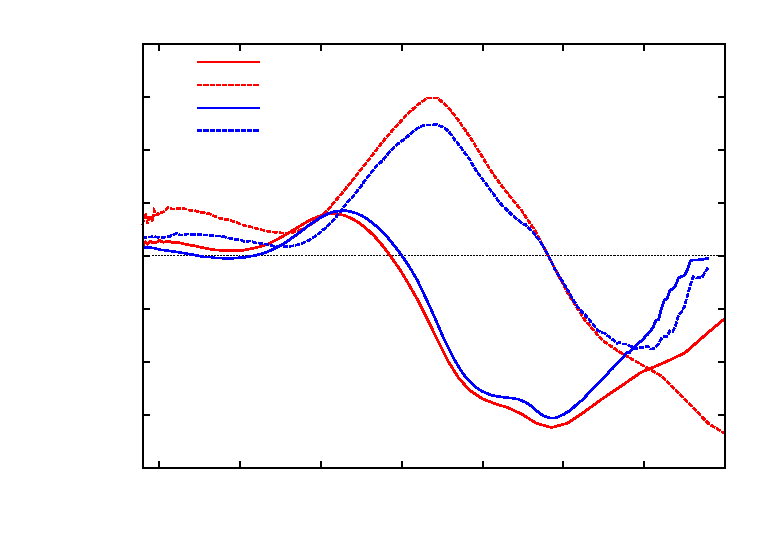
\includegraphics{grafy/PLD186}}%
    \gplfronttext
  \end{picture}%
\endgroup

\caption{Spektrum polárního Kerrova jevu vzorku PLD186. Červené křivky odpovídají metodě zkřížených polarizátorl, modré pak modulační metodě.}
\label{sPLD186}
\end{figure}

\begin{figure}
% GNUPLOT: LaTeX picture with Postscript
\begingroup
  \makeatletter
  \providecommand\color[2][]{%
    \GenericError{(gnuplot) \space\space\space\@spaces}{%
      Package color not loaded in conjunction with
      terminal option `colourtext'%
    }{See the gnuplot documentation for explanation.%
    }{Either use 'blacktext' in gnuplot or load the package
      color.sty in LaTeX.}%
    \renewcommand\color[2][]{}%
  }%
  \providecommand\includegraphics[2][]{%
    \GenericError{(gnuplot) \space\space\space\@spaces}{%
      Package graphicx or graphics not loaded%
    }{See the gnuplot documentation for explanation.%
    }{The gnuplot epslatex terminal needs graphicx.sty or graphics.sty.}%
    \renewcommand\includegraphics[2][]{}%
  }%
  \providecommand\rotatebox[2]{#2}%
  \@ifundefined{ifGPcolor}{%
    \newif\ifGPcolor
    \GPcolorfalse
  }{}%
  \@ifundefined{ifGPblacktext}{%
    \newif\ifGPblacktext
    \GPblacktexttrue
  }{}%
  % define a \g@addto@macro without @ in the name:
  \let\gplgaddtomacro\g@addto@macro
  % define empty templates for all commands taking text:
  \gdef\gplbacktext{}%
  \gdef\gplfronttext{}%
  \makeatother
  \ifGPblacktext
    % no textcolor at all
    \def\colorrgb#1{}%
    \def\colorgray#1{}%
  \else
    % gray or color?
    \ifGPcolor
      \def\colorrgb#1{\color[rgb]{#1}}%
      \def\colorgray#1{\color[gray]{#1}}%
      \expandafter\def\csname LTw\endcsname{\color{white}}%
      \expandafter\def\csname LTb\endcsname{\color{black}}%
      \expandafter\def\csname LTa\endcsname{\color{black}}%
      \expandafter\def\csname LT0\endcsname{\color[rgb]{1,0,0}}%
      \expandafter\def\csname LT1\endcsname{\color[rgb]{0,1,0}}%
      \expandafter\def\csname LT2\endcsname{\color[rgb]{0,0,1}}%
      \expandafter\def\csname LT3\endcsname{\color[rgb]{1,0,1}}%
      \expandafter\def\csname LT4\endcsname{\color[rgb]{0,1,1}}%
      \expandafter\def\csname LT5\endcsname{\color[rgb]{1,1,0}}%
      \expandafter\def\csname LT6\endcsname{\color[rgb]{0,0,0}}%
      \expandafter\def\csname LT7\endcsname{\color[rgb]{1,0.3,0}}%
      \expandafter\def\csname LT8\endcsname{\color[rgb]{0.5,0.5,0.5}}%
    \else
      % gray
      \def\colorrgb#1{\color{black}}%
      \def\colorgray#1{\color[gray]{#1}}%
      \expandafter\def\csname LTw\endcsname{\color{white}}%
      \expandafter\def\csname LTb\endcsname{\color{black}}%
      \expandafter\def\csname LTa\endcsname{\color{black}}%
      \expandafter\def\csname LT0\endcsname{\color{black}}%
      \expandafter\def\csname LT1\endcsname{\color{black}}%
      \expandafter\def\csname LT2\endcsname{\color{black}}%
      \expandafter\def\csname LT3\endcsname{\color{black}}%
      \expandafter\def\csname LT4\endcsname{\color{black}}%
      \expandafter\def\csname LT5\endcsname{\color{black}}%
      \expandafter\def\csname LT6\endcsname{\color{black}}%
      \expandafter\def\csname LT7\endcsname{\color{black}}%
      \expandafter\def\csname LT8\endcsname{\color{black}}%
    \fi
  \fi
  \setlength{\unitlength}{0.0500bp}%
  \begin{picture}(7200.00,5040.00)%
    \gplgaddtomacro\gplbacktext{%
      \csname LTb\endcsname%
      \put(990,704){\makebox(0,0)[r]{\strut{}-0.2}}%
      \put(990,1213){\makebox(0,0)[r]{\strut{}-0.15}}%
      \put(990,1722){\makebox(0,0)[r]{\strut{}-0.1}}%
      \put(990,2231){\makebox(0,0)[r]{\strut{}-0.05}}%
      \put(990,2739){\makebox(0,0)[r]{\strut{} 0}}%
      \put(990,3248){\makebox(0,0)[r]{\strut{} 0.05}}%
      \put(990,3757){\makebox(0,0)[r]{\strut{} 0.1}}%
      \put(990,4266){\makebox(0,0)[r]{\strut{} 0.15}}%
      \put(990,4775){\makebox(0,0)[r]{\strut{} 0.2}}%
      \put(1282,484){\makebox(0,0){\strut{} 1.5}}%
      \put(2080,484){\makebox(0,0){\strut{} 2}}%
      \put(2878,484){\makebox(0,0){\strut{} 2.5}}%
      \put(3676,484){\makebox(0,0){\strut{} 3}}%
      \put(4474,484){\makebox(0,0){\strut{} 3.5}}%
      \put(5273,484){\makebox(0,0){\strut{} 4}}%
      \put(6071,484){\makebox(0,0){\strut{} 4.5}}%
      \put(6869,484){\makebox(0,0){\strut{} 5}}%
      \put(308,2739){\rotatebox{-270}{\makebox(0,0){\strut{}}}}%
      \put(3995,154){\makebox(0,0){\strut{}$E$/eV}}%
    }%
    \gplgaddtomacro\gplfronttext{%
      \csname LTb\endcsname%
      \put(3102,4602){\makebox(0,0)[r]{\strut{}$\theta^1_K$}}%
      \csname LTb\endcsname%
      \put(3102,4382){\makebox(0,0)[r]{\strut{}$\epsilon^1_K$}}%
    }%
    \gplbacktext
    \put(0,0){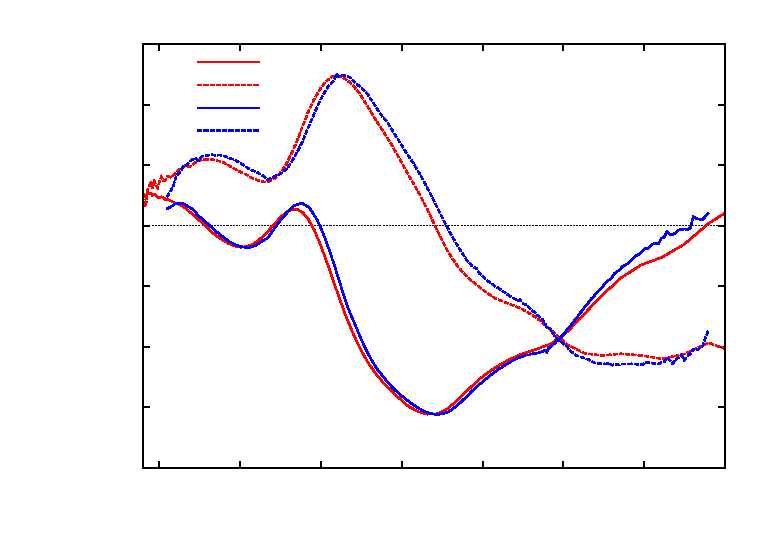
\includegraphics{PLD202}}%
    \gplfronttext
  \end{picture}%
\endgroup

\caption{Spektrum polárního Kerrova jevu vzorku PLD202. Červené křivky odpovídají metodě zkřížených polarizátorl, modré pak modulační metodě.}
\label{sPLD202}
\end{figure}

\begin{figure}
% GNUPLOT: LaTeX picture with Postscript
\begingroup
  \makeatletter
  \providecommand\color[2][]{%
    \GenericError{(gnuplot) \space\space\space\@spaces}{%
      Package color not loaded in conjunction with
      terminal option `colourtext'%
    }{See the gnuplot documentation for explanation.%
    }{Either use 'blacktext' in gnuplot or load the package
      color.sty in LaTeX.}%
    \renewcommand\color[2][]{}%
  }%
  \providecommand\includegraphics[2][]{%
    \GenericError{(gnuplot) \space\space\space\@spaces}{%
      Package graphicx or graphics not loaded%
    }{See the gnuplot documentation for explanation.%
    }{The gnuplot epslatex terminal needs graphicx.sty or graphics.sty.}%
    \renewcommand\includegraphics[2][]{}%
  }%
  \providecommand\rotatebox[2]{#2}%
  \@ifundefined{ifGPcolor}{%
    \newif\ifGPcolor
    \GPcolortrue
  }{}%
  \@ifundefined{ifGPblacktext}{%
    \newif\ifGPblacktext
    \GPblacktexttrue
  }{}%
  % define a \g@addto@macro without @ in the name:
  \let\gplgaddtomacro\g@addto@macro
  % define empty templates for all commands taking text:
  \gdef\gplbacktext{}%
  \gdef\gplfronttext{}%
  \makeatother
  \ifGPblacktext
    % no textcolor at all
    \def\colorrgb#1{}%
    \def\colorgray#1{}%
  \else
    % gray or color?
    \ifGPcolor
      \def\colorrgb#1{\color[rgb]{#1}}%
      \def\colorgray#1{\color[gray]{#1}}%
      \expandafter\def\csname LTw\endcsname{\color{white}}%
      \expandafter\def\csname LTb\endcsname{\color{black}}%
      \expandafter\def\csname LTa\endcsname{\color{black}}%
      \expandafter\def\csname LT0\endcsname{\color[rgb]{1,0,0}}%
      \expandafter\def\csname LT1\endcsname{\color[rgb]{0,1,0}}%
      \expandafter\def\csname LT2\endcsname{\color[rgb]{0,0,1}}%
      \expandafter\def\csname LT3\endcsname{\color[rgb]{1,0,1}}%
      \expandafter\def\csname LT4\endcsname{\color[rgb]{0,1,1}}%
      \expandafter\def\csname LT5\endcsname{\color[rgb]{1,1,0}}%
      \expandafter\def\csname LT6\endcsname{\color[rgb]{0,0,0}}%
      \expandafter\def\csname LT7\endcsname{\color[rgb]{1,0.3,0}}%
      \expandafter\def\csname LT8\endcsname{\color[rgb]{0.5,0.5,0.5}}%
    \else
      % gray
      \def\colorrgb#1{\color{black}}%
      \def\colorgray#1{\color[gray]{#1}}%
      \expandafter\def\csname LTw\endcsname{\color{white}}%
      \expandafter\def\csname LTb\endcsname{\color{black}}%
      \expandafter\def\csname LTa\endcsname{\color{black}}%
      \expandafter\def\csname LT0\endcsname{\color{black}}%
      \expandafter\def\csname LT1\endcsname{\color{black}}%
      \expandafter\def\csname LT2\endcsname{\color{black}}%
      \expandafter\def\csname LT3\endcsname{\color{black}}%
      \expandafter\def\csname LT4\endcsname{\color{black}}%
      \expandafter\def\csname LT5\endcsname{\color{black}}%
      \expandafter\def\csname LT6\endcsname{\color{black}}%
      \expandafter\def\csname LT7\endcsname{\color{black}}%
      \expandafter\def\csname LT8\endcsname{\color{black}}%
    \fi
  \fi
  \setlength{\unitlength}{0.0500bp}%
  \begin{picture}(7200.00,5040.00)%
    \gplgaddtomacro\gplbacktext{%
      \csname LTb\endcsname%
      \put(1078,704){\makebox(0,0)[r]{\strut{}-0.2}}%
      \put(1078,1213){\makebox(0,0)[r]{\strut{}-0.15}}%
      \put(1078,1722){\makebox(0,0)[r]{\strut{}-0.1}}%
      \put(1078,2231){\makebox(0,0)[r]{\strut{}-0.05}}%
      \put(1078,2740){\makebox(0,0)[r]{\strut{} 0}}%
      \put(1078,3248){\makebox(0,0)[r]{\strut{} 0.05}}%
      \put(1078,3757){\makebox(0,0)[r]{\strut{} 0.1}}%
      \put(1078,4266){\makebox(0,0)[r]{\strut{} 0.15}}%
      \put(1078,4775){\makebox(0,0)[r]{\strut{} 0.2}}%
      \put(1897,484){\makebox(0,0){\strut{} 2}}%
      \put(2878,484){\makebox(0,0){\strut{} 2.5}}%
      \put(3859,484){\makebox(0,0){\strut{} 3}}%
      \put(4841,484){\makebox(0,0){\strut{} 3.5}}%
      \put(5822,484){\makebox(0,0){\strut{} 4}}%
      \put(6803,484){\makebox(0,0){\strut{} 4.5}}%
      \csname LTb\endcsname%
      \put(176,2739){\rotatebox{-270}{\makebox(0,0){\strut{}Polární Kerrův jev [deg.]}}}%
      \put(4006,154){\makebox(0,0){\strut{}$E$ [eV]}}%
    }%
    \gplgaddtomacro\gplfronttext{%
      \csname LTb\endcsname%
      \put(1606,4602){\makebox(0,0)[r]{\strut{}$\theta_K$}}%
      \csname LTb\endcsname%
      \put(1606,4382){\makebox(0,0)[r]{\strut{}$\epsilon_K$}}%
      \csname LTb\endcsname%
      \put(1606,4162){\makebox(0,0)[r]{\strut{}$\theta_K$}}%
      \csname LTb\endcsname%
      \put(1606,3942){\makebox(0,0)[r]{\strut{}$\epsilon_K$}}%
    }%
    \gplbacktext
    \put(0,0){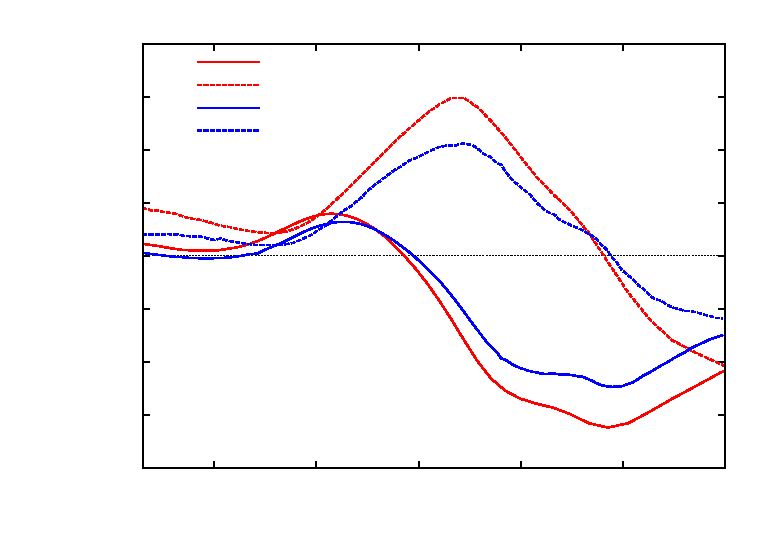
\includegraphics{PLD186t}}%
    \gplfronttext
  \end{picture}%
\endgroup

\caption{Spektrum polárního Kerrova jevu vzorku PLD186. Červené křivky odpovídají metodě zkřížených polarizátorl, modré pak teoretickým hodnotám.}
\label{sPLD186t}
\end{figure}

\begin{figure}
% GNUPLOT: LaTeX picture with Postscript
\begingroup
  \makeatletter
  \providecommand\color[2][]{%
    \GenericError{(gnuplot) \space\space\space\@spaces}{%
      Package color not loaded in conjunction with
      terminal option `colourtext'%
    }{See the gnuplot documentation for explanation.%
    }{Either use 'blacktext' in gnuplot or load the package
      color.sty in LaTeX.}%
    \renewcommand\color[2][]{}%
  }%
  \providecommand\includegraphics[2][]{%
    \GenericError{(gnuplot) \space\space\space\@spaces}{%
      Package graphicx or graphics not loaded%
    }{See the gnuplot documentation for explanation.%
    }{The gnuplot epslatex terminal needs graphicx.sty or graphics.sty.}%
    \renewcommand\includegraphics[2][]{}%
  }%
  \providecommand\rotatebox[2]{#2}%
  \@ifundefined{ifGPcolor}{%
    \newif\ifGPcolor
    \GPcolortrue
  }{}%
  \@ifundefined{ifGPblacktext}{%
    \newif\ifGPblacktext
    \GPblacktexttrue
  }{}%
  % define a \g@addto@macro without @ in the name:
  \let\gplgaddtomacro\g@addto@macro
  % define empty templates for all commands taking text:
  \gdef\gplbacktext{}%
  \gdef\gplfronttext{}%
  \makeatother
  \ifGPblacktext
    % no textcolor at all
    \def\colorrgb#1{}%
    \def\colorgray#1{}%
  \else
    % gray or color?
    \ifGPcolor
      \def\colorrgb#1{\color[rgb]{#1}}%
      \def\colorgray#1{\color[gray]{#1}}%
      \expandafter\def\csname LTw\endcsname{\color{white}}%
      \expandafter\def\csname LTb\endcsname{\color{black}}%
      \expandafter\def\csname LTa\endcsname{\color{black}}%
      \expandafter\def\csname LT0\endcsname{\color[rgb]{1,0,0}}%
      \expandafter\def\csname LT1\endcsname{\color[rgb]{0,1,0}}%
      \expandafter\def\csname LT2\endcsname{\color[rgb]{0,0,1}}%
      \expandafter\def\csname LT3\endcsname{\color[rgb]{1,0,1}}%
      \expandafter\def\csname LT4\endcsname{\color[rgb]{0,1,1}}%
      \expandafter\def\csname LT5\endcsname{\color[rgb]{1,1,0}}%
      \expandafter\def\csname LT6\endcsname{\color[rgb]{0,0,0}}%
      \expandafter\def\csname LT7\endcsname{\color[rgb]{1,0.3,0}}%
      \expandafter\def\csname LT8\endcsname{\color[rgb]{0.5,0.5,0.5}}%
    \else
      % gray
      \def\colorrgb#1{\color{black}}%
      \def\colorgray#1{\color[gray]{#1}}%
      \expandafter\def\csname LTw\endcsname{\color{white}}%
      \expandafter\def\csname LTb\endcsname{\color{black}}%
      \expandafter\def\csname LTa\endcsname{\color{black}}%
      \expandafter\def\csname LT0\endcsname{\color{black}}%
      \expandafter\def\csname LT1\endcsname{\color{black}}%
      \expandafter\def\csname LT2\endcsname{\color{black}}%
      \expandafter\def\csname LT3\endcsname{\color{black}}%
      \expandafter\def\csname LT4\endcsname{\color{black}}%
      \expandafter\def\csname LT5\endcsname{\color{black}}%
      \expandafter\def\csname LT6\endcsname{\color{black}}%
      \expandafter\def\csname LT7\endcsname{\color{black}}%
      \expandafter\def\csname LT8\endcsname{\color{black}}%
    \fi
  \fi
  \setlength{\unitlength}{0.0500bp}%
  \begin{picture}(7200.00,5040.00)%
    \gplgaddtomacro\gplbacktext{%
      \csname LTb\endcsname%
      \put(1078,704){\makebox(0,0)[r]{\strut{}-0.25}}%
      \put(1078,1156){\makebox(0,0)[r]{\strut{}-0.2}}%
      \put(1078,1609){\makebox(0,0)[r]{\strut{}-0.15}}%
      \put(1078,2061){\makebox(0,0)[r]{\strut{}-0.1}}%
      \put(1078,2513){\makebox(0,0)[r]{\strut{}-0.05}}%
      \put(1078,2966){\makebox(0,0)[r]{\strut{} 0}}%
      \put(1078,3418){\makebox(0,0)[r]{\strut{} 0.05}}%
      \put(1078,3870){\makebox(0,0)[r]{\strut{} 0.1}}%
      \put(1078,4323){\makebox(0,0)[r]{\strut{} 0.15}}%
      \put(1078,4775){\makebox(0,0)[r]{\strut{} 0.2}}%
      \put(1897,484){\makebox(0,0){\strut{} 2}}%
      \put(2878,484){\makebox(0,0){\strut{} 2.5}}%
      \put(3859,484){\makebox(0,0){\strut{} 3}}%
      \put(4841,484){\makebox(0,0){\strut{} 3.5}}%
      \put(5822,484){\makebox(0,0){\strut{} 4}}%
      \put(6803,484){\makebox(0,0){\strut{} 4.5}}%
      \csname LTb\endcsname%
      \put(176,2739){\rotatebox{-270}{\makebox(0,0){\strut{}Polární Kerrův jev [deg.]}}}%
      \put(4006,154){\makebox(0,0){\strut{}$E$ [eV]}}%
    }%
    \gplgaddtomacro\gplfronttext{%
      \csname LTb\endcsname%
      \put(1606,1537){\makebox(0,0)[r]{\strut{}$\theta_K$}}%
      \csname LTb\endcsname%
      \put(1606,1317){\makebox(0,0)[r]{\strut{}$\epsilon_K$}}%
      \csname LTb\endcsname%
      \put(1606,1097){\makebox(0,0)[r]{\strut{}$\theta_K$}}%
      \csname LTb\endcsname%
      \put(1606,877){\makebox(0,0)[r]{\strut{}$\epsilon_K$}}%
    }%
    \gplbacktext
    \put(0,0){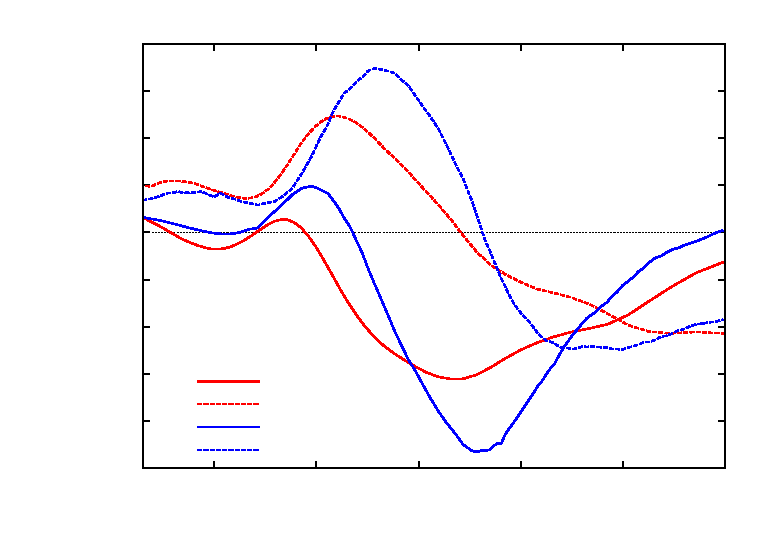
\includegraphics{PLD202t}}%
    \gplfronttext
  \end{picture}%
\endgroup

\caption{Spektrum polárního Kerrova jevu vzorku PLD202. Červené křivky odpovídají metodě zkřížených polarizátorl, modré pak teoretickým hodnotám.}
\label{sPLD202t}
\end{figure}
\section{Kobaltové feritové tenké vrstvy}
Další velmi intenzivně studovanou skupinou materiálů jsou oxidy železa.
Tyto materiály mají dobrý potenciál pro použití v mikrovlnných zařízeních a  pro magnetooptický zápis. 
Jejich hlavní předností je vysoká Curiova teplota, vysoká koercitiva a velká magnetická anizotropie. 

Tenké vrstvy kobaltového feritu (CoFe$_2$O$_4$) jsou obzvláště zajímavé díky vysoké hustotě magnetického zápisu.
Naše vzorky byli připravené metodou PLD na substrát z amorfního taveného křemene. K odpaření terčíku byly použity 5 ns dlouhé pulsy Nd:YAG laseru. 
Deponování námi zkoumaných vzorků probáhala za pokojové teploty, následně byly vzorky zahřáty na 750 (CoF-RT-A750) resp. 1100 (CoF-RT-A1100) 
stupňů Celsia. Tato teplota byla udržována po dobu dvou hodin, po kterých se vzorky nechaly schladit opět na pokojovou teplotu. Tloušťka vrstev je 110 nm.

Změřená spektra koblatových feritů jsou zobrazena na obrázcích \ref{sCoF-RT-A750} a \ref{sCoF-RT-A1100}. Z nich je dobře vidět, že vzorek je až do přibližně 2.7 eV značně transparentní, protože na spektru vznikl interferenčí obrazec pro tenkou vrstvu. Výsledky metod se v této oblasti liší, protože úhel dopadu se u metod odlišuje, což má za následek zdánlivý rozdíl 
v tloušťce vzorku. 

Nad 2.5 eV je spektrum už typické pro ferity. Konkrétně má velmi podobné spektrum jako lithný nebo mědnatý ferit. \cite{ferity} 
Rozdíl amplitud je dán již zmíněnou nižší citlivostí fotonásobiče modulační metody.

Dále je vidět vliv teploty, při které byly vzorky deponovány, na spektrum vzorku. Při vysokých teplotách totiž zřejmě dochází k materiálovým změnám, které mají za následek pokles magnetizace ve vzorku, a tím pádem i magnetooptické odezvy.


\begin{figure}
% GNUPLOT: LaTeX picture with Postscript
\begingroup
  \makeatletter
  \providecommand\color[2][]{%
    \GenericError{(gnuplot) \space\space\space\@spaces}{%
      Package color not loaded in conjunction with
      terminal option `colourtext'%
    }{See the gnuplot documentation for explanation.%
    }{Either use 'blacktext' in gnuplot or load the package
      color.sty in LaTeX.}%
    \renewcommand\color[2][]{}%
  }%
  \providecommand\includegraphics[2][]{%
    \GenericError{(gnuplot) \space\space\space\@spaces}{%
      Package graphicx or graphics not loaded%
    }{See the gnuplot documentation for explanation.%
    }{The gnuplot epslatex terminal needs graphicx.sty or graphics.sty.}%
    \renewcommand\includegraphics[2][]{}%
  }%
  \providecommand\rotatebox[2]{#2}%
  \@ifundefined{ifGPcolor}{%
    \newif\ifGPcolor
    \GPcolortrue
  }{}%
  \@ifundefined{ifGPblacktext}{%
    \newif\ifGPblacktext
    \GPblacktexttrue
  }{}%
  % define a \g@addto@macro without @ in the name:
  \let\gplgaddtomacro\g@addto@macro
  % define empty templates for all commands taking text:
  \gdef\gplbacktext{}%
  \gdef\gplfronttext{}%
  \makeatother
  \ifGPblacktext
    % no textcolor at all
    \def\colorrgb#1{}%
    \def\colorgray#1{}%
  \else
    % gray or color?
    \ifGPcolor
      \def\colorrgb#1{\color[rgb]{#1}}%
      \def\colorgray#1{\color[gray]{#1}}%
      \expandafter\def\csname LTw\endcsname{\color{white}}%
      \expandafter\def\csname LTb\endcsname{\color{black}}%
      \expandafter\def\csname LTa\endcsname{\color{black}}%
      \expandafter\def\csname LT0\endcsname{\color[rgb]{1,0,0}}%
      \expandafter\def\csname LT1\endcsname{\color[rgb]{0,1,0}}%
      \expandafter\def\csname LT2\endcsname{\color[rgb]{0,0,1}}%
      \expandafter\def\csname LT3\endcsname{\color[rgb]{1,0,1}}%
      \expandafter\def\csname LT4\endcsname{\color[rgb]{0,1,1}}%
      \expandafter\def\csname LT5\endcsname{\color[rgb]{1,1,0}}%
      \expandafter\def\csname LT6\endcsname{\color[rgb]{0,0,0}}%
      \expandafter\def\csname LT7\endcsname{\color[rgb]{1,0.3,0}}%
      \expandafter\def\csname LT8\endcsname{\color[rgb]{0.5,0.5,0.5}}%
    \else
      % gray
      \def\colorrgb#1{\color{black}}%
      \def\colorgray#1{\color[gray]{#1}}%
      \expandafter\def\csname LTw\endcsname{\color{white}}%
      \expandafter\def\csname LTb\endcsname{\color{black}}%
      \expandafter\def\csname LTa\endcsname{\color{black}}%
      \expandafter\def\csname LT0\endcsname{\color{black}}%
      \expandafter\def\csname LT1\endcsname{\color{black}}%
      \expandafter\def\csname LT2\endcsname{\color{black}}%
      \expandafter\def\csname LT3\endcsname{\color{black}}%
      \expandafter\def\csname LT4\endcsname{\color{black}}%
      \expandafter\def\csname LT5\endcsname{\color{black}}%
      \expandafter\def\csname LT6\endcsname{\color{black}}%
      \expandafter\def\csname LT7\endcsname{\color{black}}%
      \expandafter\def\csname LT8\endcsname{\color{black}}%
    \fi
  \fi
  \setlength{\unitlength}{0.0500bp}%
  \begin{picture}(7200.00,5040.00)%
    \gplgaddtomacro\gplbacktext{%
      \csname LTb\endcsname%
      \put(946,704){\makebox(0,0)[r]{\strut{}-0.6}}%
      \put(946,1383){\makebox(0,0)[r]{\strut{}-0.4}}%
      \put(946,2061){\makebox(0,0)[r]{\strut{}-0.2}}%
      \put(946,2740){\makebox(0,0)[r]{\strut{} 0}}%
      \put(946,3418){\makebox(0,0)[r]{\strut{} 0.2}}%
      \put(946,4097){\makebox(0,0)[r]{\strut{} 0.4}}%
      \put(946,4775){\makebox(0,0)[r]{\strut{} 0.6}}%
      \put(1257,484){\makebox(0,0){\strut{} 1.5}}%
      \put(2151,484){\makebox(0,0){\strut{} 2}}%
      \put(3046,484){\makebox(0,0){\strut{} 2.5}}%
      \put(3941,484){\makebox(0,0){\strut{} 3}}%
      \put(4835,484){\makebox(0,0){\strut{} 3.5}}%
      \put(5730,484){\makebox(0,0){\strut{} 4}}%
      \put(6624,484){\makebox(0,0){\strut{} 4.5}}%
      \csname LTb\endcsname%
      \put(176,2739){\rotatebox{-270}{\makebox(0,0){\strut{}Polární Kerrův jev [deg.]}}}%
      \put(3940,154){\makebox(0,0){\strut{}$E$ [eV]}}%
    }%
    \gplgaddtomacro\gplfronttext{%
      \csname LTb\endcsname%
      \put(5816,4602){\makebox(0,0)[r]{\strut{}$\theta_K$}}%
      \csname LTb\endcsname%
      \put(5816,4382){\makebox(0,0)[r]{\strut{}$\epsilon_K$}}%
      \csname LTb\endcsname%
      \put(5816,4162){\makebox(0,0)[r]{\strut{}$\theta_K$}}%
      \csname LTb\endcsname%
      \put(5816,3942){\makebox(0,0)[r]{\strut{}$\epsilon_K$}}%
    }%
    \gplbacktext
    \put(0,0){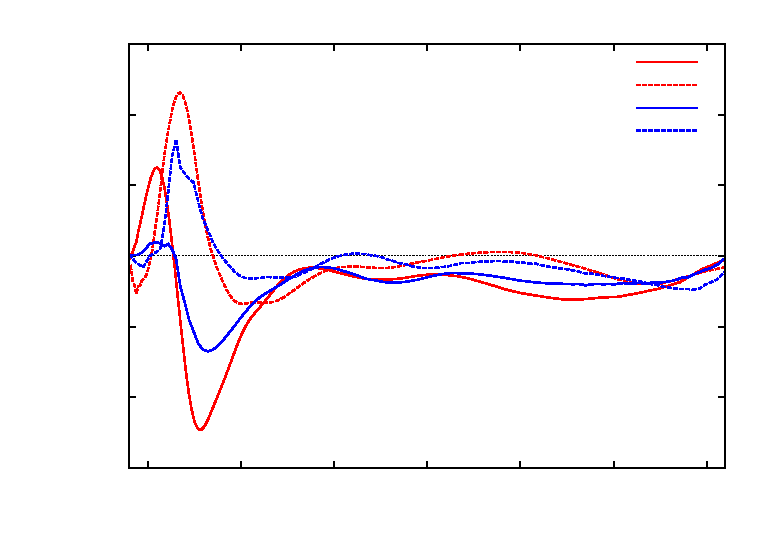
\includegraphics{CoF-RT-A750}}%
    \gplfronttext
  \end{picture}%
\endgroup

\caption{Spektrum polárního Kerrova jevu vzorku CoF-RT-A750. Červené křivky odpovídají metodě zkřížených polarizátorl, modré pak modulační metodě.}
\label{sCoF-RT-A750}
\end{figure}

\begin{figure}
% GNUPLOT: LaTeX picture with Postscript
\begingroup
  \makeatletter
  \providecommand\color[2][]{%
    \GenericError{(gnuplot) \space\space\space\@spaces}{%
      Package color not loaded in conjunction with
      terminal option `colourtext'%
    }{See the gnuplot documentation for explanation.%
    }{Either use 'blacktext' in gnuplot or load the package
      color.sty in LaTeX.}%
    \renewcommand\color[2][]{}%
  }%
  \providecommand\includegraphics[2][]{%
    \GenericError{(gnuplot) \space\space\space\@spaces}{%
      Package graphicx or graphics not loaded%
    }{See the gnuplot documentation for explanation.%
    }{The gnuplot epslatex terminal needs graphicx.sty or graphics.sty.}%
    \renewcommand\includegraphics[2][]{}%
  }%
  \providecommand\rotatebox[2]{#2}%
  \@ifundefined{ifGPcolor}{%
    \newif\ifGPcolor
    \GPcolorfalse
  }{}%
  \@ifundefined{ifGPblacktext}{%
    \newif\ifGPblacktext
    \GPblacktexttrue
  }{}%
  % define a \g@addto@macro without @ in the name:
  \let\gplgaddtomacro\g@addto@macro
  % define empty templates for all commands taking text:
  \gdef\gplbacktext{}%
  \gdef\gplfronttext{}%
  \makeatother
  \ifGPblacktext
    % no textcolor at all
    \def\colorrgb#1{}%
    \def\colorgray#1{}%
  \else
    % gray or color?
    \ifGPcolor
      \def\colorrgb#1{\color[rgb]{#1}}%
      \def\colorgray#1{\color[gray]{#1}}%
      \expandafter\def\csname LTw\endcsname{\color{white}}%
      \expandafter\def\csname LTb\endcsname{\color{black}}%
      \expandafter\def\csname LTa\endcsname{\color{black}}%
      \expandafter\def\csname LT0\endcsname{\color[rgb]{1,0,0}}%
      \expandafter\def\csname LT1\endcsname{\color[rgb]{0,1,0}}%
      \expandafter\def\csname LT2\endcsname{\color[rgb]{0,0,1}}%
      \expandafter\def\csname LT3\endcsname{\color[rgb]{1,0,1}}%
      \expandafter\def\csname LT4\endcsname{\color[rgb]{0,1,1}}%
      \expandafter\def\csname LT5\endcsname{\color[rgb]{1,1,0}}%
      \expandafter\def\csname LT6\endcsname{\color[rgb]{0,0,0}}%
      \expandafter\def\csname LT7\endcsname{\color[rgb]{1,0.3,0}}%
      \expandafter\def\csname LT8\endcsname{\color[rgb]{0.5,0.5,0.5}}%
    \else
      % gray
      \def\colorrgb#1{\color{black}}%
      \def\colorgray#1{\color[gray]{#1}}%
      \expandafter\def\csname LTw\endcsname{\color{white}}%
      \expandafter\def\csname LTb\endcsname{\color{black}}%
      \expandafter\def\csname LTa\endcsname{\color{black}}%
      \expandafter\def\csname LT0\endcsname{\color{black}}%
      \expandafter\def\csname LT1\endcsname{\color{black}}%
      \expandafter\def\csname LT2\endcsname{\color{black}}%
      \expandafter\def\csname LT3\endcsname{\color{black}}%
      \expandafter\def\csname LT4\endcsname{\color{black}}%
      \expandafter\def\csname LT5\endcsname{\color{black}}%
      \expandafter\def\csname LT6\endcsname{\color{black}}%
      \expandafter\def\csname LT7\endcsname{\color{black}}%
      \expandafter\def\csname LT8\endcsname{\color{black}}%
    \fi
  \fi
  \setlength{\unitlength}{0.0500bp}%
  \begin{picture}(7200.00,5040.00)%
    \gplgaddtomacro\gplbacktext{%
      \csname LTb\endcsname%
      \put(1078,704){\makebox(0,0)[r]{\strut{}-0.4}}%
      \put(1078,1213){\makebox(0,0)[r]{\strut{}-0.3}}%
      \put(1078,1722){\makebox(0,0)[r]{\strut{}-0.2}}%
      \put(1078,2231){\makebox(0,0)[r]{\strut{}-0.1}}%
      \put(1078,2739){\makebox(0,0)[r]{\strut{} 0}}%
      \put(1078,3248){\makebox(0,0)[r]{\strut{} 0.1}}%
      \put(1078,3757){\makebox(0,0)[r]{\strut{} 0.2}}%
      \put(1078,4266){\makebox(0,0)[r]{\strut{} 0.3}}%
      \put(1078,4775){\makebox(0,0)[r]{\strut{} 0.4}}%
      \put(1367,484){\makebox(0,0){\strut{} 1.5}}%
      \put(2153,484){\makebox(0,0){\strut{} 2}}%
      \put(2939,484){\makebox(0,0){\strut{} 2.5}}%
      \put(3725,484){\makebox(0,0){\strut{} 3}}%
      \put(4511,484){\makebox(0,0){\strut{} 3.5}}%
      \put(5297,484){\makebox(0,0){\strut{} 4}}%
      \put(6083,484){\makebox(0,0){\strut{} 4.5}}%
      \put(6869,484){\makebox(0,0){\strut{} 5}}%
      \put(308,2739){\rotatebox{-270}{\makebox(0,0){\strut{}Polární Kerrův jev [deg.]}}}%
      \put(4039,154){\makebox(0,0){\strut{}$E$/eV}}%
    }%
    \gplgaddtomacro\gplfronttext{%
      \csname LTb\endcsname%
      \put(5882,4602){\makebox(0,0)[r]{\strut{}$\theta^1_K$}}%
      \csname LTb\endcsname%
      \put(5882,4382){\makebox(0,0)[r]{\strut{}$\epsilon^1_K$}}%
      \csname LTb\endcsname%
      \put(5882,4162){\makebox(0,0)[r]{\strut{}$\theta^2_K$}}%
      \csname LTb\endcsname%
      \put(5882,3942){\makebox(0,0)[r]{\strut{}$\epsilon^2_K$}}%
    }%
    \gplbacktext
    \put(0,0){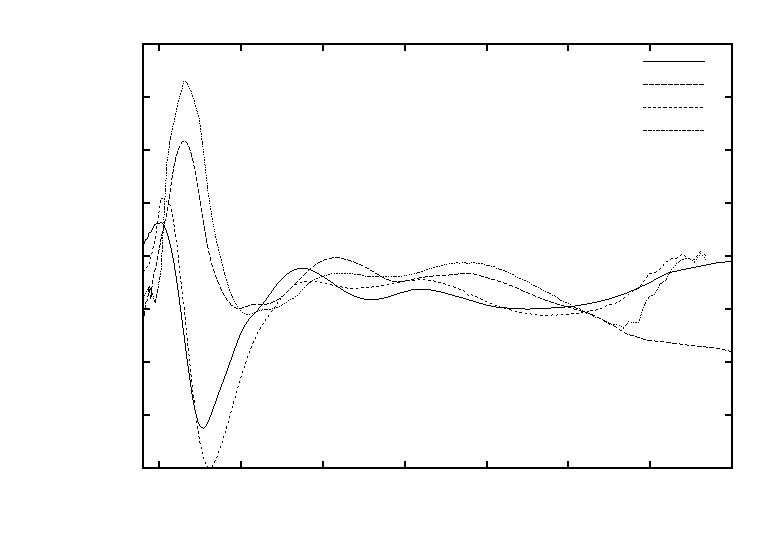
\includegraphics{grafy/CoF-RT-A1100}}%
    \gplfronttext
  \end{picture}%
\endgroup

\caption{Spektrum polárního Kerrova jevu vzorku CoF-RT-A1100. Červené křivky odpovídají metodě zkřížených polarizátorl, modré pak modulační metodě.}
\label{sCoF-RT-A1100}
\end{figure}

\section{Heuslerovy slitiny}
Jako poslední typ vzorků jsme použily zástupce z Heuslerovývh slitin. Tyto vzorky mají opět 
skvělé vlastnosti pro použití v oblasti spintroniky.  Námi zkoumané slitiny byly různou směsí kobaltu, 
železa a křemíku. Ze všech zástupců zkoumaných Heuslerových slitin mají tyto výrazně nejvyšší Curiovu 
teplotu ($\sim 1100$K). Pro srovnání se Curiova teplota Fe$_2$MnSi se pohybuje pod pokojovou teplotou.

Tyto materiály se vyrábí za pomoci nízkoteplotní molekulární svazkové epitaxie. Ve zkratce se při této 
metodě v oddělených komorách zahřívají jednotlivé koponenty. Jejich výpary vstupují do hlavní komory, ve které je velmi vysoké vakuum, kde následně kondenzují na substrátu. 
Rychlost růstu se pohybuje pod 3000 nm za hodinu, což umožňuje výrobu velmi tenkých filmů.

Deponování našich vzorků probíhalo na substrát MgO. Na něm byla deponována nejprve 5 nm tenká vrstva chrómu, následně 20 nm slitiny a navrchu 2 nm MgO. Poměry kovů ve slitinách byli 7:5 (CoFeSi1) a 2:1 (CoFeSi2) v prospěch kobaltu.

Spektra vzorků Heuslerových slitin jsou na obrázcích \ref{sCoFeSi1} a \ref{sCoFeSi2}. Rozdílná velikost amplitud efektů je dána použitím různých magnetů. 
Magnet první z metod totiž nevytváří dostatečně velké pole pro nasycení vzorku. Porovnáním tvarů spekter však vidíme, že si výsledky obou metod si spektrálně odpovídají.

Ze spekter je také dobře vidět, že vetší přítomnost železa na úkor kobaltu má za následek větší efekt. Pokles eplipticit v UV oblasti je opět dán menší citlivostí 
fotonásobiče modulační metody.

\begin{figure}
% GNUPLOT: LaTeX picture with Postscript
\begingroup
  \makeatletter
  \providecommand\color[2][]{%
    \GenericError{(gnuplot) \space\space\space\@spaces}{%
      Package color not loaded in conjunction with
      terminal option `colourtext'%
    }{See the gnuplot documentation for explanation.%
    }{Either use 'blacktext' in gnuplot or load the package
      color.sty in LaTeX.}%
    \renewcommand\color[2][]{}%
  }%
  \providecommand\includegraphics[2][]{%
    \GenericError{(gnuplot) \space\space\space\@spaces}{%
      Package graphicx or graphics not loaded%
    }{See the gnuplot documentation for explanation.%
    }{The gnuplot epslatex terminal needs graphicx.sty or graphics.sty.}%
    \renewcommand\includegraphics[2][]{}%
  }%
  \providecommand\rotatebox[2]{#2}%
  \@ifundefined{ifGPcolor}{%
    \newif\ifGPcolor
    \GPcolorfalse
  }{}%
  \@ifundefined{ifGPblacktext}{%
    \newif\ifGPblacktext
    \GPblacktexttrue
  }{}%
  % define a \g@addto@macro without @ in the name:
  \let\gplgaddtomacro\g@addto@macro
  % define empty templates for all commands taking text:
  \gdef\gplbacktext{}%
  \gdef\gplfronttext{}%
  \makeatother
  \ifGPblacktext
    % no textcolor at all
    \def\colorrgb#1{}%
    \def\colorgray#1{}%
  \else
    % gray or color?
    \ifGPcolor
      \def\colorrgb#1{\color[rgb]{#1}}%
      \def\colorgray#1{\color[gray]{#1}}%
      \expandafter\def\csname LTw\endcsname{\color{white}}%
      \expandafter\def\csname LTb\endcsname{\color{black}}%
      \expandafter\def\csname LTa\endcsname{\color{black}}%
      \expandafter\def\csname LT0\endcsname{\color[rgb]{1,0,0}}%
      \expandafter\def\csname LT1\endcsname{\color[rgb]{0,1,0}}%
      \expandafter\def\csname LT2\endcsname{\color[rgb]{0,0,1}}%
      \expandafter\def\csname LT3\endcsname{\color[rgb]{1,0,1}}%
      \expandafter\def\csname LT4\endcsname{\color[rgb]{0,1,1}}%
      \expandafter\def\csname LT5\endcsname{\color[rgb]{1,1,0}}%
      \expandafter\def\csname LT6\endcsname{\color[rgb]{0,0,0}}%
      \expandafter\def\csname LT7\endcsname{\color[rgb]{1,0.3,0}}%
      \expandafter\def\csname LT8\endcsname{\color[rgb]{0.5,0.5,0.5}}%
    \else
      % gray
      \def\colorrgb#1{\color{black}}%
      \def\colorgray#1{\color[gray]{#1}}%
      \expandafter\def\csname LTw\endcsname{\color{white}}%
      \expandafter\def\csname LTb\endcsname{\color{black}}%
      \expandafter\def\csname LTa\endcsname{\color{black}}%
      \expandafter\def\csname LT0\endcsname{\color{black}}%
      \expandafter\def\csname LT1\endcsname{\color{black}}%
      \expandafter\def\csname LT2\endcsname{\color{black}}%
      \expandafter\def\csname LT3\endcsname{\color{black}}%
      \expandafter\def\csname LT4\endcsname{\color{black}}%
      \expandafter\def\csname LT5\endcsname{\color{black}}%
      \expandafter\def\csname LT6\endcsname{\color{black}}%
      \expandafter\def\csname LT7\endcsname{\color{black}}%
      \expandafter\def\csname LT8\endcsname{\color{black}}%
    \fi
  \fi
  \setlength{\unitlength}{0.0500bp}%
  \begin{picture}(7200.00,5040.00)%
    \gplgaddtomacro\gplbacktext{%
      \csname LTb\endcsname%
      \put(1122,704){\makebox(0,0)[r]{\strut{}-0.008}}%
      \put(1122,1213){\makebox(0,0)[r]{\strut{}-0.006}}%
      \put(1122,1722){\makebox(0,0)[r]{\strut{}-0.004}}%
      \put(1122,2231){\makebox(0,0)[r]{\strut{}-0.002}}%
      \put(1122,2740){\makebox(0,0)[r]{\strut{} 0}}%
      \put(1122,3248){\makebox(0,0)[r]{\strut{} 0.002}}%
      \put(1122,3757){\makebox(0,0)[r]{\strut{} 0.004}}%
      \put(1122,4266){\makebox(0,0)[r]{\strut{} 0.006}}%
      \put(1122,4775){\makebox(0,0)[r]{\strut{} 0.008}}%
      \put(1410,484){\makebox(0,0){\strut{} 1.5}}%
      \put(2190,484){\makebox(0,0){\strut{} 2}}%
      \put(2970,484){\makebox(0,0){\strut{} 2.5}}%
      \put(3750,484){\makebox(0,0){\strut{} 3}}%
      \put(4529,484){\makebox(0,0){\strut{} 3.5}}%
      \put(5309,484){\makebox(0,0){\strut{} 4}}%
      \put(6089,484){\makebox(0,0){\strut{} 4.5}}%
      \put(6869,484){\makebox(0,0){\strut{} 5}}%
      \put(308,2739){\rotatebox{-270}{\makebox(0,0){\strut{}}}}%
      \put(4061,154){\makebox(0,0){\strut{}$E$/eV}}%
    }%
    \gplgaddtomacro\gplfronttext{%
      \csname LTb\endcsname%
      \put(2970,4602){\makebox(0,0)[r]{\strut{}$\theta_K$}}%
      \csname LTb\endcsname%
      \put(2970,4382){\makebox(0,0)[r]{\strut{}$\epsilon_K$}}%
    }%
    \gplbacktext
    \put(0,0){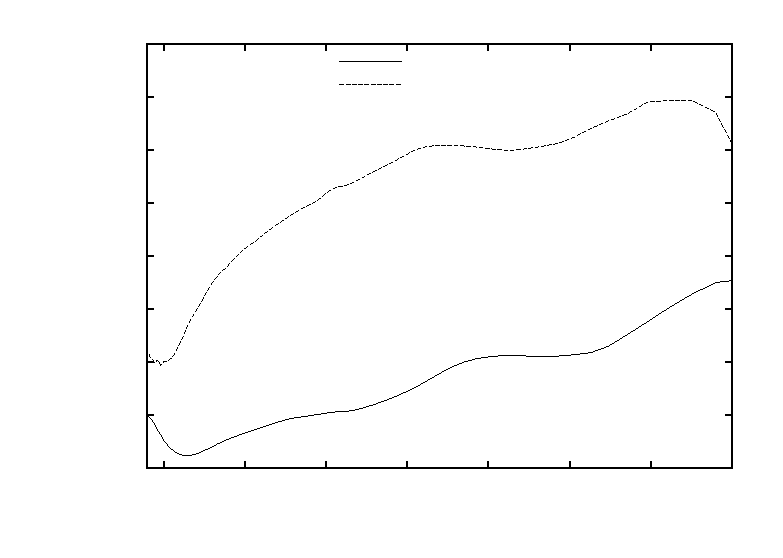
\includegraphics{CoFeSi1}}%
    \gplfronttext
  \end{picture}%
\endgroup

\caption{Spektrum polárního Kerrova jevu vzorku CoFeSi1. Červené křivky odpovídají metodě zkřížených polarizátorl, modré pak modulační metodě.}
\label{sCoFeSi1}
\end{figure}

\begin{figure}
% GNUPLOT: LaTeX picture with Postscript
\begingroup
  \makeatletter
  \providecommand\color[2][]{%
    \GenericError{(gnuplot) \space\space\space\@spaces}{%
      Package color not loaded in conjunction with
      terminal option `colourtext'%
    }{See the gnuplot documentation for explanation.%
    }{Either use 'blacktext' in gnuplot or load the package
      color.sty in LaTeX.}%
    \renewcommand\color[2][]{}%
  }%
  \providecommand\includegraphics[2][]{%
    \GenericError{(gnuplot) \space\space\space\@spaces}{%
      Package graphicx or graphics not loaded%
    }{See the gnuplot documentation for explanation.%
    }{The gnuplot epslatex terminal needs graphicx.sty or graphics.sty.}%
    \renewcommand\includegraphics[2][]{}%
  }%
  \providecommand\rotatebox[2]{#2}%
  \@ifundefined{ifGPcolor}{%
    \newif\ifGPcolor
    \GPcolortrue
  }{}%
  \@ifundefined{ifGPblacktext}{%
    \newif\ifGPblacktext
    \GPblacktexttrue
  }{}%
  % define a \g@addto@macro without @ in the name:
  \let\gplgaddtomacro\g@addto@macro
  % define empty templates for all commands taking text:
  \gdef\gplbacktext{}%
  \gdef\gplfronttext{}%
  \makeatother
  \ifGPblacktext
    % no textcolor at all
    \def\colorrgb#1{}%
    \def\colorgray#1{}%
  \else
    % gray or color?
    \ifGPcolor
      \def\colorrgb#1{\color[rgb]{#1}}%
      \def\colorgray#1{\color[gray]{#1}}%
      \expandafter\def\csname LTw\endcsname{\color{white}}%
      \expandafter\def\csname LTb\endcsname{\color{black}}%
      \expandafter\def\csname LTa\endcsname{\color{black}}%
      \expandafter\def\csname LT0\endcsname{\color[rgb]{1,0,0}}%
      \expandafter\def\csname LT1\endcsname{\color[rgb]{0,1,0}}%
      \expandafter\def\csname LT2\endcsname{\color[rgb]{0,0,1}}%
      \expandafter\def\csname LT3\endcsname{\color[rgb]{1,0,1}}%
      \expandafter\def\csname LT4\endcsname{\color[rgb]{0,1,1}}%
      \expandafter\def\csname LT5\endcsname{\color[rgb]{1,1,0}}%
      \expandafter\def\csname LT6\endcsname{\color[rgb]{0,0,0}}%
      \expandafter\def\csname LT7\endcsname{\color[rgb]{1,0.3,0}}%
      \expandafter\def\csname LT8\endcsname{\color[rgb]{0.5,0.5,0.5}}%
    \else
      % gray
      \def\colorrgb#1{\color{black}}%
      \def\colorgray#1{\color[gray]{#1}}%
      \expandafter\def\csname LTw\endcsname{\color{white}}%
      \expandafter\def\csname LTb\endcsname{\color{black}}%
      \expandafter\def\csname LTa\endcsname{\color{black}}%
      \expandafter\def\csname LT0\endcsname{\color{black}}%
      \expandafter\def\csname LT1\endcsname{\color{black}}%
      \expandafter\def\csname LT2\endcsname{\color{black}}%
      \expandafter\def\csname LT3\endcsname{\color{black}}%
      \expandafter\def\csname LT4\endcsname{\color{black}}%
      \expandafter\def\csname LT5\endcsname{\color{black}}%
      \expandafter\def\csname LT6\endcsname{\color{black}}%
      \expandafter\def\csname LT7\endcsname{\color{black}}%
      \expandafter\def\csname LT8\endcsname{\color{black}}%
    \fi
  \fi
  \setlength{\unitlength}{0.0500bp}%
  \begin{picture}(7200.00,5040.00)%
    \gplgaddtomacro\gplbacktext{%
      \csname LTb\endcsname%
      \put(1078,704){\makebox(0,0)[r]{\strut{}-0.3}}%
      \put(1078,1156){\makebox(0,0)[r]{\strut{}-0.25}}%
      \put(1078,1609){\makebox(0,0)[r]{\strut{}-0.2}}%
      \put(1078,2061){\makebox(0,0)[r]{\strut{}-0.15}}%
      \put(1078,2513){\makebox(0,0)[r]{\strut{}-0.1}}%
      \put(1078,2966){\makebox(0,0)[r]{\strut{}-0.05}}%
      \put(1078,3418){\makebox(0,0)[r]{\strut{} 0}}%
      \put(1078,3870){\makebox(0,0)[r]{\strut{} 0.05}}%
      \put(1078,4323){\makebox(0,0)[r]{\strut{} 0.1}}%
      \put(1078,4775){\makebox(0,0)[r]{\strut{} 0.15}}%
      \put(1379,484){\makebox(0,0){\strut{} 1.5}}%
      \put(2227,484){\makebox(0,0){\strut{} 2}}%
      \put(3074,484){\makebox(0,0){\strut{} 2.5}}%
      \put(3922,484){\makebox(0,0){\strut{} 3}}%
      \put(4769,484){\makebox(0,0){\strut{} 3.5}}%
      \put(5617,484){\makebox(0,0){\strut{} 4}}%
      \put(6464,484){\makebox(0,0){\strut{} 4.5}}%
      \csname LTb\endcsname%
      \put(176,2739){\rotatebox{-270}{\makebox(0,0){\strut{}Polární Kerrův jev [deg.]}}}%
      \put(4006,154){\makebox(0,0){\strut{}$E$ [eV]}}%
    }%
    \gplgaddtomacro\gplfronttext{%
      \csname LTb\endcsname%
      \put(5816,1537){\makebox(0,0)[r]{\strut{}$\theta_K$}}%
      \csname LTb\endcsname%
      \put(5816,1317){\makebox(0,0)[r]{\strut{}$\epsilon_K$}}%
      \csname LTb\endcsname%
      \put(5816,1097){\makebox(0,0)[r]{\strut{}$\theta_K$}}%
      \csname LTb\endcsname%
      \put(5816,877){\makebox(0,0)[r]{\strut{}$\epsilon_K$}}%
    }%
    \gplbacktext
    \put(0,0){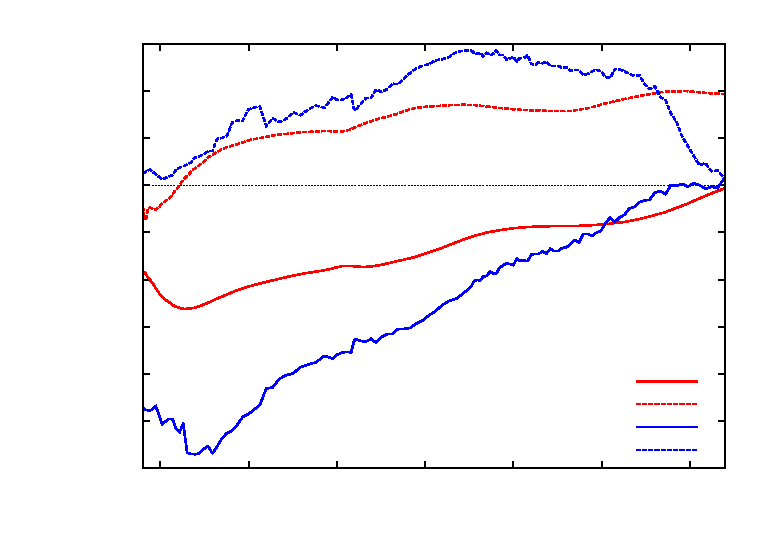
\includegraphics{CoFeSi2}}%
    \gplfronttext
  \end{picture}%
\endgroup

\caption{Spektrum polárního Kerrova jevu vzorku CoFeSi2. Červené křivky odpovídají metodě zkřížených polarizátorl, modré pak modulační metodě.}
\label{sCoFeSi2}
\end{figure}

%\chapter{Výsledky}
\section{Heuslerovy slitiny}
Spektra vzorků Heuslerových slitin jsou na obrázcích (\ref{sCoFeSi1}) a (\ref{sCoFeSi2}). Na nich můžete dobře vidět srovnání výsledku obou použitých metod. Tvar spekter je zcela totožný, až na odchylku u CoFeSi2 okolo hodnoty 2.5 eV, kdy se do měření obtiskla nestálost intenzity lampy. Amplituda efektu se liší, protože magnet aparatury se zkříženými polarizátory vytváří nedostatečné magnetické pole pro nasycení vzorků. Ze spekter je také dobře vidět, že vetší přítomnost železa oroti kobaltu ve vzorku má za následek větší efekt.

\section{Kobaltové ferity}
Výsledky měření koblatových feritů jsou na obrázcích (\ref{sCoF-RT-A750}) a (\ref{sCoF-RT-A1100}). Z nich je dobře vidět, že vzorek je až do hodnoty 2.5 eV průhledný, protože na spektru vznikl interferenčí obrazec pro tenkou vrstvu. Dále je vidět, že s depoziční teplota nemá příliš velký vliv na výsledný efekt vzorku.

\section{PLD}
Spektra vzorků PLD můžeme srovnat s teoretickými hodnotami, které jsme vypočítali dle vztahu (\ref{teor kerr}). Výsledky jsou na obrázcích (\ref{sPLD189}) a (\ref{sPLD202}), na kterých je dobře vidět, že spektra získaná oběmy experimentálnímy metodami velmi dobře odpovídají teoretickému předpokladu.

\begin{figure}
% GNUPLOT: LaTeX picture with Postscript
\begingroup
  \makeatletter
  \providecommand\color[2][]{%
    \GenericError{(gnuplot) \space\space\space\@spaces}{%
      Package color not loaded in conjunction with
      terminal option `colourtext'%
    }{See the gnuplot documentation for explanation.%
    }{Either use 'blacktext' in gnuplot or load the package
      color.sty in LaTeX.}%
    \renewcommand\color[2][]{}%
  }%
  \providecommand\includegraphics[2][]{%
    \GenericError{(gnuplot) \space\space\space\@spaces}{%
      Package graphicx or graphics not loaded%
    }{See the gnuplot documentation for explanation.%
    }{The gnuplot epslatex terminal needs graphicx.sty or graphics.sty.}%
    \renewcommand\includegraphics[2][]{}%
  }%
  \providecommand\rotatebox[2]{#2}%
  \@ifundefined{ifGPcolor}{%
    \newif\ifGPcolor
    \GPcolorfalse
  }{}%
  \@ifundefined{ifGPblacktext}{%
    \newif\ifGPblacktext
    \GPblacktexttrue
  }{}%
  % define a \g@addto@macro without @ in the name:
  \let\gplgaddtomacro\g@addto@macro
  % define empty templates for all commands taking text:
  \gdef\gplbacktext{}%
  \gdef\gplfronttext{}%
  \makeatother
  \ifGPblacktext
    % no textcolor at all
    \def\colorrgb#1{}%
    \def\colorgray#1{}%
  \else
    % gray or color?
    \ifGPcolor
      \def\colorrgb#1{\color[rgb]{#1}}%
      \def\colorgray#1{\color[gray]{#1}}%
      \expandafter\def\csname LTw\endcsname{\color{white}}%
      \expandafter\def\csname LTb\endcsname{\color{black}}%
      \expandafter\def\csname LTa\endcsname{\color{black}}%
      \expandafter\def\csname LT0\endcsname{\color[rgb]{1,0,0}}%
      \expandafter\def\csname LT1\endcsname{\color[rgb]{0,1,0}}%
      \expandafter\def\csname LT2\endcsname{\color[rgb]{0,0,1}}%
      \expandafter\def\csname LT3\endcsname{\color[rgb]{1,0,1}}%
      \expandafter\def\csname LT4\endcsname{\color[rgb]{0,1,1}}%
      \expandafter\def\csname LT5\endcsname{\color[rgb]{1,1,0}}%
      \expandafter\def\csname LT6\endcsname{\color[rgb]{0,0,0}}%
      \expandafter\def\csname LT7\endcsname{\color[rgb]{1,0.3,0}}%
      \expandafter\def\csname LT8\endcsname{\color[rgb]{0.5,0.5,0.5}}%
    \else
      % gray
      \def\colorrgb#1{\color{black}}%
      \def\colorgray#1{\color[gray]{#1}}%
      \expandafter\def\csname LTw\endcsname{\color{white}}%
      \expandafter\def\csname LTb\endcsname{\color{black}}%
      \expandafter\def\csname LTa\endcsname{\color{black}}%
      \expandafter\def\csname LT0\endcsname{\color{black}}%
      \expandafter\def\csname LT1\endcsname{\color{black}}%
      \expandafter\def\csname LT2\endcsname{\color{black}}%
      \expandafter\def\csname LT3\endcsname{\color{black}}%
      \expandafter\def\csname LT4\endcsname{\color{black}}%
      \expandafter\def\csname LT5\endcsname{\color{black}}%
      \expandafter\def\csname LT6\endcsname{\color{black}}%
      \expandafter\def\csname LT7\endcsname{\color{black}}%
      \expandafter\def\csname LT8\endcsname{\color{black}}%
    \fi
  \fi
  \setlength{\unitlength}{0.0500bp}%
  \begin{picture}(7200.00,5040.00)%
    \gplgaddtomacro\gplbacktext{%
      \csname LTb\endcsname%
      \put(1210,704){\makebox(0,0)[r]{\strut{}-0.2}}%
      \put(1210,1213){\makebox(0,0)[r]{\strut{}-0.15}}%
      \put(1210,1722){\makebox(0,0)[r]{\strut{}-0.1}}%
      \put(1210,2231){\makebox(0,0)[r]{\strut{}-0.05}}%
      \put(1210,2739){\makebox(0,0)[r]{\strut{} 0}}%
      \put(1210,3248){\makebox(0,0)[r]{\strut{} 0.05}}%
      \put(1210,3757){\makebox(0,0)[r]{\strut{} 0.1}}%
      \put(1210,4266){\makebox(0,0)[r]{\strut{} 0.15}}%
      \put(1210,4775){\makebox(0,0)[r]{\strut{} 0.2}}%
      \put(1496,484){\makebox(0,0){\strut{} 1.5}}%
      \put(2263,484){\makebox(0,0){\strut{} 2}}%
      \put(3031,484){\makebox(0,0){\strut{} 2.5}}%
      \put(3798,484){\makebox(0,0){\strut{} 3}}%
      \put(4566,484){\makebox(0,0){\strut{} 3.5}}%
      \put(5334,484){\makebox(0,0){\strut{} 4}}%
      \put(6101,484){\makebox(0,0){\strut{} 4.5}}%
      \put(6869,484){\makebox(0,0){\strut{} 5}}%
      \put(308,2739){\rotatebox{-270}{\makebox(0,0){\strut{}Polární Kerrův jev [deg.]}}}%
      \put(4105,154){\makebox(0,0){\strut{}$E$/eV}}%
    }%
    \gplgaddtomacro\gplfronttext{%
      \csname LTb\endcsname%
      \put(5882,4602){\makebox(0,0)[r]{\strut{}$\theta^1_K$}}%
      \csname LTb\endcsname%
      \put(5882,4382){\makebox(0,0)[r]{\strut{}$\epsilon^1_K$}}%
      \csname LTb\endcsname%
      \put(5882,4162){\makebox(0,0)[r]{\strut{}$\theta^2_K$}}%
      \csname LTb\endcsname%
      \put(5882,3942){\makebox(0,0)[r]{\strut{}$\epsilon^2_K$}}%
    }%
    \gplbacktext
    \put(0,0){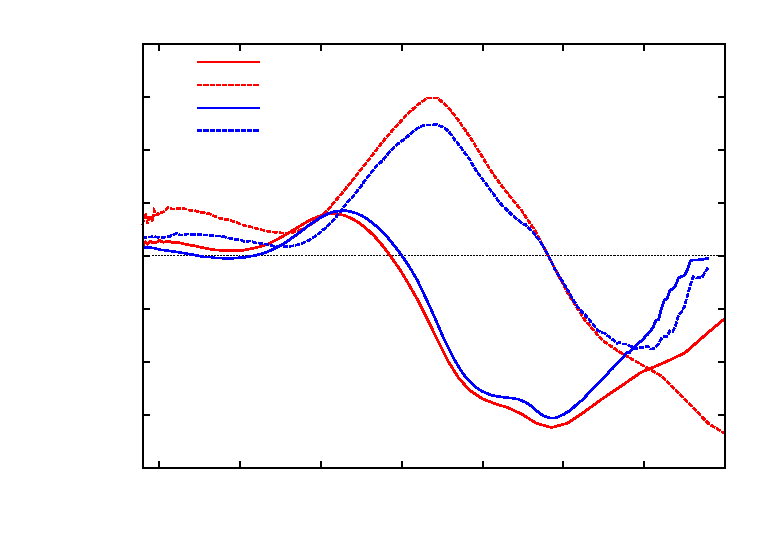
\includegraphics{grafy/PLD186}}%
    \gplfronttext
  \end{picture}%
\endgroup

\caption{Spektrumn vzorku PLD186}
\label{sPLD189}
\end{figure}

%\begin{figure}
%% GNUPLOT: LaTeX picture with Postscript
\begingroup
  \makeatletter
  \providecommand\color[2][]{%
    \GenericError{(gnuplot) \space\space\space\@spaces}{%
      Package color not loaded in conjunction with
      terminal option `colourtext'%
    }{See the gnuplot documentation for explanation.%
    }{Either use 'blacktext' in gnuplot or load the package
      color.sty in LaTeX.}%
    \renewcommand\color[2][]{}%
  }%
  \providecommand\includegraphics[2][]{%
    \GenericError{(gnuplot) \space\space\space\@spaces}{%
      Package graphicx or graphics not loaded%
    }{See the gnuplot documentation for explanation.%
    }{The gnuplot epslatex terminal needs graphicx.sty or graphics.sty.}%
    \renewcommand\includegraphics[2][]{}%
  }%
  \providecommand\rotatebox[2]{#2}%
  \@ifundefined{ifGPcolor}{%
    \newif\ifGPcolor
    \GPcolorfalse
  }{}%
  \@ifundefined{ifGPblacktext}{%
    \newif\ifGPblacktext
    \GPblacktexttrue
  }{}%
  % define a \g@addto@macro without @ in the name:
  \let\gplgaddtomacro\g@addto@macro
  % define empty templates for all commands taking text:
  \gdef\gplbacktext{}%
  \gdef\gplfronttext{}%
  \makeatother
  \ifGPblacktext
    % no textcolor at all
    \def\colorrgb#1{}%
    \def\colorgray#1{}%
  \else
    % gray or color?
    \ifGPcolor
      \def\colorrgb#1{\color[rgb]{#1}}%
      \def\colorgray#1{\color[gray]{#1}}%
      \expandafter\def\csname LTw\endcsname{\color{white}}%
      \expandafter\def\csname LTb\endcsname{\color{black}}%
      \expandafter\def\csname LTa\endcsname{\color{black}}%
      \expandafter\def\csname LT0\endcsname{\color[rgb]{1,0,0}}%
      \expandafter\def\csname LT1\endcsname{\color[rgb]{0,1,0}}%
      \expandafter\def\csname LT2\endcsname{\color[rgb]{0,0,1}}%
      \expandafter\def\csname LT3\endcsname{\color[rgb]{1,0,1}}%
      \expandafter\def\csname LT4\endcsname{\color[rgb]{0,1,1}}%
      \expandafter\def\csname LT5\endcsname{\color[rgb]{1,1,0}}%
      \expandafter\def\csname LT6\endcsname{\color[rgb]{0,0,0}}%
      \expandafter\def\csname LT7\endcsname{\color[rgb]{1,0.3,0}}%
      \expandafter\def\csname LT8\endcsname{\color[rgb]{0.5,0.5,0.5}}%
    \else
      % gray
      \def\colorrgb#1{\color{black}}%
      \def\colorgray#1{\color[gray]{#1}}%
      \expandafter\def\csname LTw\endcsname{\color{white}}%
      \expandafter\def\csname LTb\endcsname{\color{black}}%
      \expandafter\def\csname LTa\endcsname{\color{black}}%
      \expandafter\def\csname LT0\endcsname{\color{black}}%
      \expandafter\def\csname LT1\endcsname{\color{black}}%
      \expandafter\def\csname LT2\endcsname{\color{black}}%
      \expandafter\def\csname LT3\endcsname{\color{black}}%
      \expandafter\def\csname LT4\endcsname{\color{black}}%
      \expandafter\def\csname LT5\endcsname{\color{black}}%
      \expandafter\def\csname LT6\endcsname{\color{black}}%
      \expandafter\def\csname LT7\endcsname{\color{black}}%
      \expandafter\def\csname LT8\endcsname{\color{black}}%
    \fi
  \fi
  \setlength{\unitlength}{0.0500bp}%
  \begin{picture}(7200.00,5040.00)%
    \gplgaddtomacro\gplbacktext{%
      \csname LTb\endcsname%
      \put(1342,704){\makebox(0,0)[r]{\strut{}-0.005}}%
      \put(1342,1286){\makebox(0,0)[r]{\strut{}-0.004}}%
      \put(1342,1867){\makebox(0,0)[r]{\strut{}-0.003}}%
      \put(1342,2449){\makebox(0,0)[r]{\strut{}-0.002}}%
      \put(1342,3030){\makebox(0,0)[r]{\strut{}-0.001}}%
      \put(1342,3612){\makebox(0,0)[r]{\strut{} 0}}%
      \put(1342,4193){\makebox(0,0)[r]{\strut{} 0.001}}%
      \put(1342,4775){\makebox(0,0)[r]{\strut{} 0.002}}%
      \put(1624,484){\makebox(0,0){\strut{} 1.5}}%
      \put(2373,484){\makebox(0,0){\strut{} 2}}%
      \put(3122,484){\makebox(0,0){\strut{} 2.5}}%
      \put(3872,484){\makebox(0,0){\strut{} 3}}%
      \put(4621,484){\makebox(0,0){\strut{} 3.5}}%
      \put(5370,484){\makebox(0,0){\strut{} 4}}%
      \put(6120,484){\makebox(0,0){\strut{} 4.5}}%
      \put(6869,484){\makebox(0,0){\strut{} 5}}%
      \put(308,2739){\rotatebox{-270}{\makebox(0,0){\strut{}$\theta_K$}}}%
      \put(4171,154){\makebox(0,0){\strut{}$E$/eV}}%
    }%
    \gplgaddtomacro\gplfronttext{%
    }%
    \gplbacktext
    \put(0,0){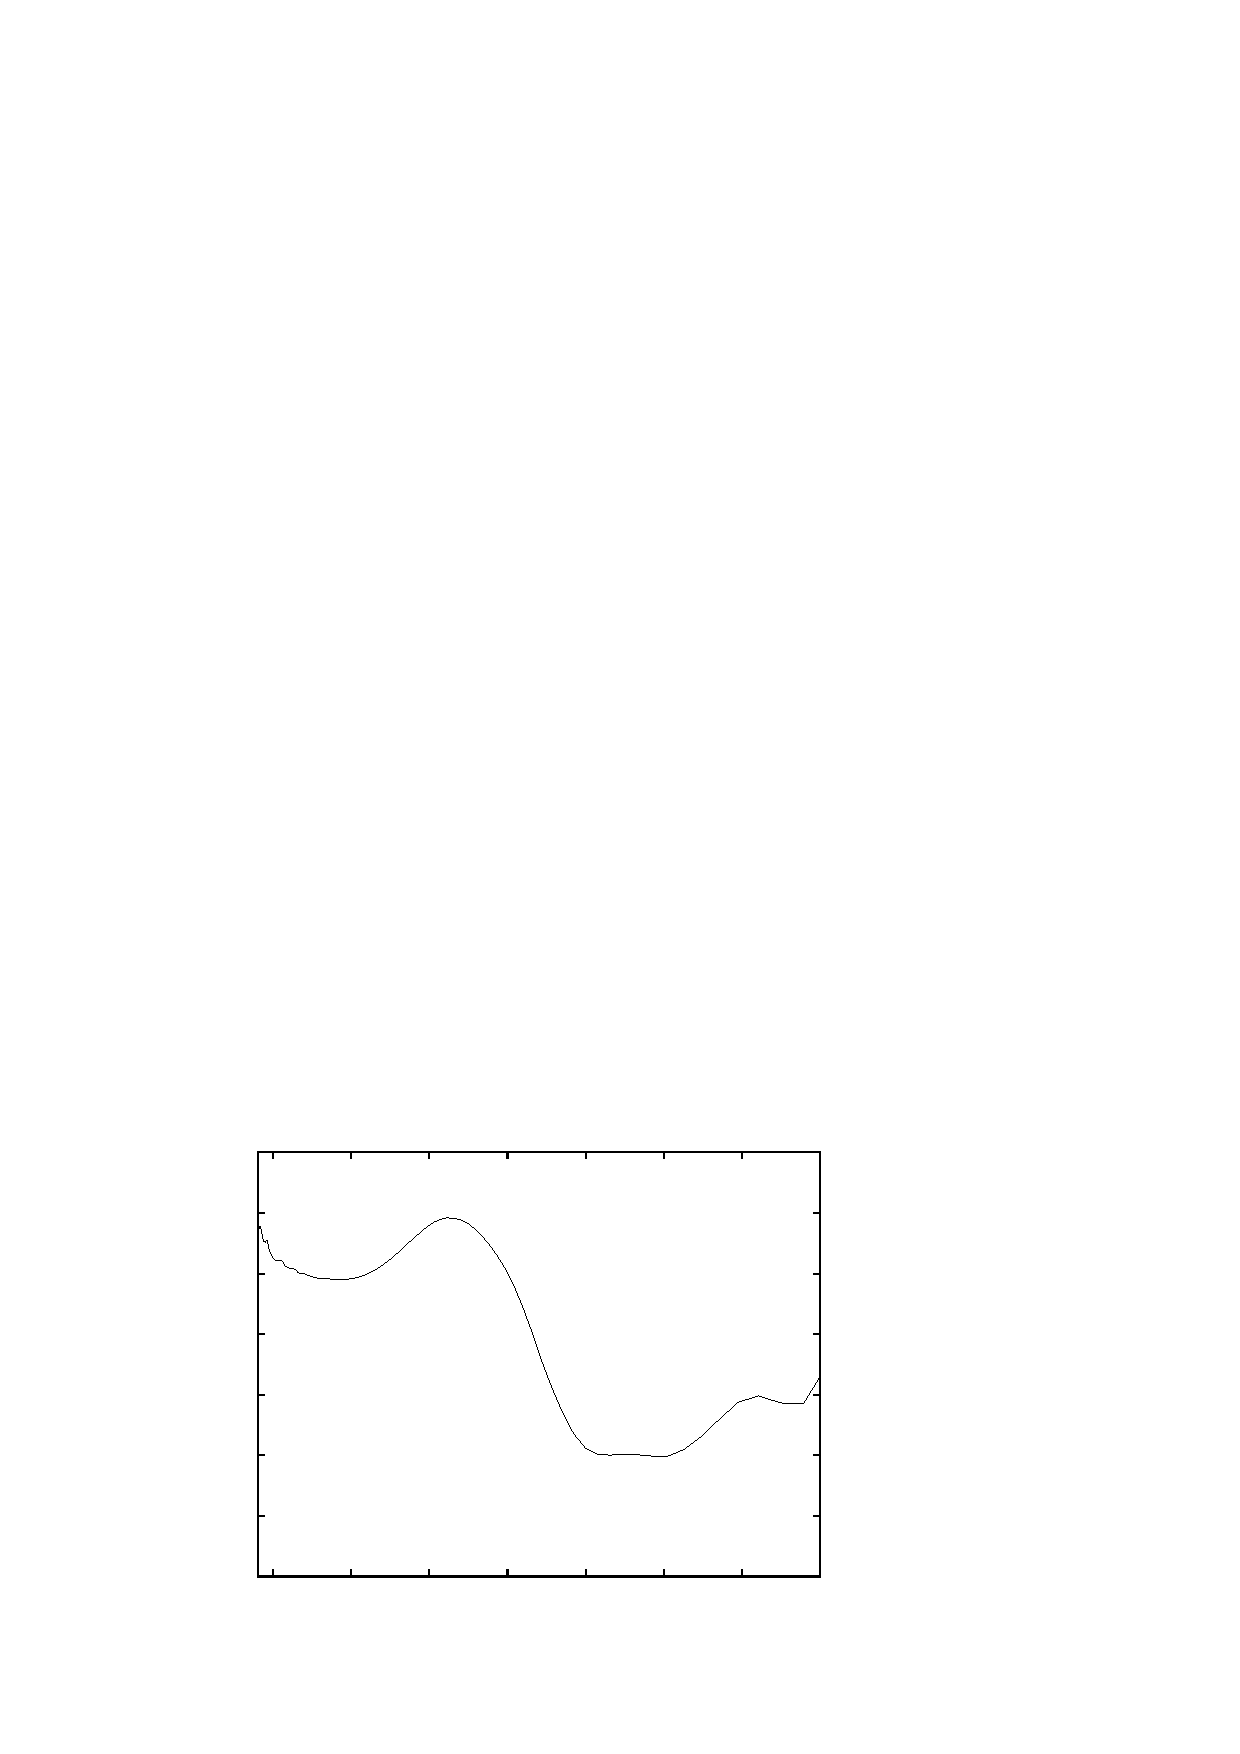
\includegraphics{PLD194}}%
    \gplfronttext
  \end{picture}%
\endgroup

%\caption{Spektrumn vzorku PLD194}
%\label{sPLD194}
%\end{figure}

\begin{figure}
%% GNUPLOT: LaTeX picture with Postscript
\begingroup
  \makeatletter
  \providecommand\color[2][]{%
    \GenericError{(gnuplot) \space\space\space\@spaces}{%
      Package color not loaded in conjunction with
      terminal option `colourtext'%
    }{See the gnuplot documentation for explanation.%
    }{Either use 'blacktext' in gnuplot or load the package
      color.sty in LaTeX.}%
    \renewcommand\color[2][]{}%
  }%
  \providecommand\includegraphics[2][]{%
    \GenericError{(gnuplot) \space\space\space\@spaces}{%
      Package graphicx or graphics not loaded%
    }{See the gnuplot documentation for explanation.%
    }{The gnuplot epslatex terminal needs graphicx.sty or graphics.sty.}%
    \renewcommand\includegraphics[2][]{}%
  }%
  \providecommand\rotatebox[2]{#2}%
  \@ifundefined{ifGPcolor}{%
    \newif\ifGPcolor
    \GPcolorfalse
  }{}%
  \@ifundefined{ifGPblacktext}{%
    \newif\ifGPblacktext
    \GPblacktexttrue
  }{}%
  % define a \g@addto@macro without @ in the name:
  \let\gplgaddtomacro\g@addto@macro
  % define empty templates for all commands taking text:
  \gdef\gplbacktext{}%
  \gdef\gplfronttext{}%
  \makeatother
  \ifGPblacktext
    % no textcolor at all
    \def\colorrgb#1{}%
    \def\colorgray#1{}%
  \else
    % gray or color?
    \ifGPcolor
      \def\colorrgb#1{\color[rgb]{#1}}%
      \def\colorgray#1{\color[gray]{#1}}%
      \expandafter\def\csname LTw\endcsname{\color{white}}%
      \expandafter\def\csname LTb\endcsname{\color{black}}%
      \expandafter\def\csname LTa\endcsname{\color{black}}%
      \expandafter\def\csname LT0\endcsname{\color[rgb]{1,0,0}}%
      \expandafter\def\csname LT1\endcsname{\color[rgb]{0,1,0}}%
      \expandafter\def\csname LT2\endcsname{\color[rgb]{0,0,1}}%
      \expandafter\def\csname LT3\endcsname{\color[rgb]{1,0,1}}%
      \expandafter\def\csname LT4\endcsname{\color[rgb]{0,1,1}}%
      \expandafter\def\csname LT5\endcsname{\color[rgb]{1,1,0}}%
      \expandafter\def\csname LT6\endcsname{\color[rgb]{0,0,0}}%
      \expandafter\def\csname LT7\endcsname{\color[rgb]{1,0.3,0}}%
      \expandafter\def\csname LT8\endcsname{\color[rgb]{0.5,0.5,0.5}}%
    \else
      % gray
      \def\colorrgb#1{\color{black}}%
      \def\colorgray#1{\color[gray]{#1}}%
      \expandafter\def\csname LTw\endcsname{\color{white}}%
      \expandafter\def\csname LTb\endcsname{\color{black}}%
      \expandafter\def\csname LTa\endcsname{\color{black}}%
      \expandafter\def\csname LT0\endcsname{\color{black}}%
      \expandafter\def\csname LT1\endcsname{\color{black}}%
      \expandafter\def\csname LT2\endcsname{\color{black}}%
      \expandafter\def\csname LT3\endcsname{\color{black}}%
      \expandafter\def\csname LT4\endcsname{\color{black}}%
      \expandafter\def\csname LT5\endcsname{\color{black}}%
      \expandafter\def\csname LT6\endcsname{\color{black}}%
      \expandafter\def\csname LT7\endcsname{\color{black}}%
      \expandafter\def\csname LT8\endcsname{\color{black}}%
    \fi
  \fi
  \setlength{\unitlength}{0.0500bp}%
  \begin{picture}(7200.00,5040.00)%
    \gplgaddtomacro\gplbacktext{%
      \csname LTb\endcsname%
      \put(990,704){\makebox(0,0)[r]{\strut{}-0.2}}%
      \put(990,1213){\makebox(0,0)[r]{\strut{}-0.15}}%
      \put(990,1722){\makebox(0,0)[r]{\strut{}-0.1}}%
      \put(990,2231){\makebox(0,0)[r]{\strut{}-0.05}}%
      \put(990,2739){\makebox(0,0)[r]{\strut{} 0}}%
      \put(990,3248){\makebox(0,0)[r]{\strut{} 0.05}}%
      \put(990,3757){\makebox(0,0)[r]{\strut{} 0.1}}%
      \put(990,4266){\makebox(0,0)[r]{\strut{} 0.15}}%
      \put(990,4775){\makebox(0,0)[r]{\strut{} 0.2}}%
      \put(1282,484){\makebox(0,0){\strut{} 1.5}}%
      \put(2080,484){\makebox(0,0){\strut{} 2}}%
      \put(2878,484){\makebox(0,0){\strut{} 2.5}}%
      \put(3676,484){\makebox(0,0){\strut{} 3}}%
      \put(4474,484){\makebox(0,0){\strut{} 3.5}}%
      \put(5273,484){\makebox(0,0){\strut{} 4}}%
      \put(6071,484){\makebox(0,0){\strut{} 4.5}}%
      \put(6869,484){\makebox(0,0){\strut{} 5}}%
      \put(308,2739){\rotatebox{-270}{\makebox(0,0){\strut{}}}}%
      \put(3995,154){\makebox(0,0){\strut{}$E$/eV}}%
    }%
    \gplgaddtomacro\gplfronttext{%
      \csname LTb\endcsname%
      \put(3102,4602){\makebox(0,0)[r]{\strut{}$\theta^1_K$}}%
      \csname LTb\endcsname%
      \put(3102,4382){\makebox(0,0)[r]{\strut{}$\epsilon^1_K$}}%
    }%
    \gplbacktext
    \put(0,0){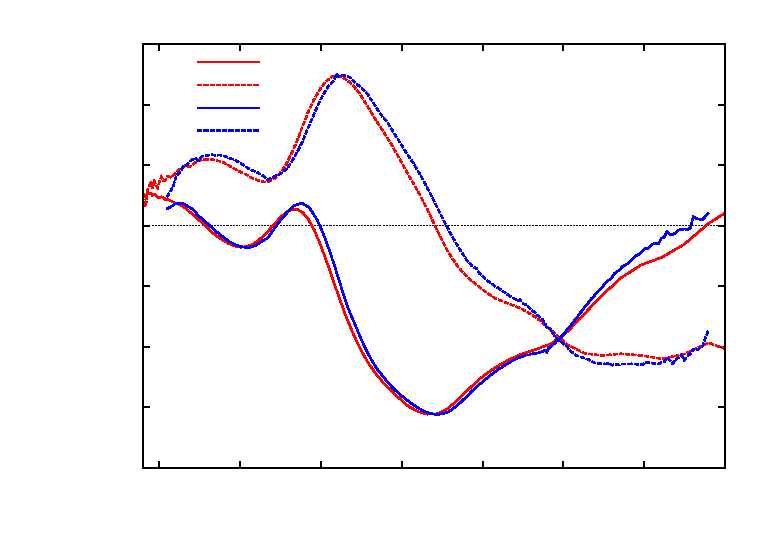
\includegraphics{PLD202}}%
    \gplfronttext
  \end{picture}%
\endgroup

\caption{Spektrumn vzorku PLD202}
\label{sPLD202}
\end{figure}

\begin{figure}
% GNUPLOT: LaTeX picture with Postscript
\begingroup
  \makeatletter
  \providecommand\color[2][]{%
    \GenericError{(gnuplot) \space\space\space\@spaces}{%
      Package color not loaded in conjunction with
      terminal option `colourtext'%
    }{See the gnuplot documentation for explanation.%
    }{Either use 'blacktext' in gnuplot or load the package
      color.sty in LaTeX.}%
    \renewcommand\color[2][]{}%
  }%
  \providecommand\includegraphics[2][]{%
    \GenericError{(gnuplot) \space\space\space\@spaces}{%
      Package graphicx or graphics not loaded%
    }{See the gnuplot documentation for explanation.%
    }{The gnuplot epslatex terminal needs graphicx.sty or graphics.sty.}%
    \renewcommand\includegraphics[2][]{}%
  }%
  \providecommand\rotatebox[2]{#2}%
  \@ifundefined{ifGPcolor}{%
    \newif\ifGPcolor
    \GPcolorfalse
  }{}%
  \@ifundefined{ifGPblacktext}{%
    \newif\ifGPblacktext
    \GPblacktexttrue
  }{}%
  % define a \g@addto@macro without @ in the name:
  \let\gplgaddtomacro\g@addto@macro
  % define empty templates for all commands taking text:
  \gdef\gplbacktext{}%
  \gdef\gplfronttext{}%
  \makeatother
  \ifGPblacktext
    % no textcolor at all
    \def\colorrgb#1{}%
    \def\colorgray#1{}%
  \else
    % gray or color?
    \ifGPcolor
      \def\colorrgb#1{\color[rgb]{#1}}%
      \def\colorgray#1{\color[gray]{#1}}%
      \expandafter\def\csname LTw\endcsname{\color{white}}%
      \expandafter\def\csname LTb\endcsname{\color{black}}%
      \expandafter\def\csname LTa\endcsname{\color{black}}%
      \expandafter\def\csname LT0\endcsname{\color[rgb]{1,0,0}}%
      \expandafter\def\csname LT1\endcsname{\color[rgb]{0,1,0}}%
      \expandafter\def\csname LT2\endcsname{\color[rgb]{0,0,1}}%
      \expandafter\def\csname LT3\endcsname{\color[rgb]{1,0,1}}%
      \expandafter\def\csname LT4\endcsname{\color[rgb]{0,1,1}}%
      \expandafter\def\csname LT5\endcsname{\color[rgb]{1,1,0}}%
      \expandafter\def\csname LT6\endcsname{\color[rgb]{0,0,0}}%
      \expandafter\def\csname LT7\endcsname{\color[rgb]{1,0.3,0}}%
      \expandafter\def\csname LT8\endcsname{\color[rgb]{0.5,0.5,0.5}}%
    \else
      % gray
      \def\colorrgb#1{\color{black}}%
      \def\colorgray#1{\color[gray]{#1}}%
      \expandafter\def\csname LTw\endcsname{\color{white}}%
      \expandafter\def\csname LTb\endcsname{\color{black}}%
      \expandafter\def\csname LTa\endcsname{\color{black}}%
      \expandafter\def\csname LT0\endcsname{\color{black}}%
      \expandafter\def\csname LT1\endcsname{\color{black}}%
      \expandafter\def\csname LT2\endcsname{\color{black}}%
      \expandafter\def\csname LT3\endcsname{\color{black}}%
      \expandafter\def\csname LT4\endcsname{\color{black}}%
      \expandafter\def\csname LT5\endcsname{\color{black}}%
      \expandafter\def\csname LT6\endcsname{\color{black}}%
      \expandafter\def\csname LT7\endcsname{\color{black}}%
      \expandafter\def\csname LT8\endcsname{\color{black}}%
    \fi
  \fi
  \setlength{\unitlength}{0.0500bp}%
  \begin{picture}(7200.00,5040.00)%
    \gplgaddtomacro\gplbacktext{%
      \csname LTb\endcsname%
      \put(1122,704){\makebox(0,0)[r]{\strut{}-0.008}}%
      \put(1122,1213){\makebox(0,0)[r]{\strut{}-0.006}}%
      \put(1122,1722){\makebox(0,0)[r]{\strut{}-0.004}}%
      \put(1122,2231){\makebox(0,0)[r]{\strut{}-0.002}}%
      \put(1122,2740){\makebox(0,0)[r]{\strut{} 0}}%
      \put(1122,3248){\makebox(0,0)[r]{\strut{} 0.002}}%
      \put(1122,3757){\makebox(0,0)[r]{\strut{} 0.004}}%
      \put(1122,4266){\makebox(0,0)[r]{\strut{} 0.006}}%
      \put(1122,4775){\makebox(0,0)[r]{\strut{} 0.008}}%
      \put(1410,484){\makebox(0,0){\strut{} 1.5}}%
      \put(2190,484){\makebox(0,0){\strut{} 2}}%
      \put(2970,484){\makebox(0,0){\strut{} 2.5}}%
      \put(3750,484){\makebox(0,0){\strut{} 3}}%
      \put(4529,484){\makebox(0,0){\strut{} 3.5}}%
      \put(5309,484){\makebox(0,0){\strut{} 4}}%
      \put(6089,484){\makebox(0,0){\strut{} 4.5}}%
      \put(6869,484){\makebox(0,0){\strut{} 5}}%
      \put(308,2739){\rotatebox{-270}{\makebox(0,0){\strut{}}}}%
      \put(4061,154){\makebox(0,0){\strut{}$E$/eV}}%
    }%
    \gplgaddtomacro\gplfronttext{%
      \csname LTb\endcsname%
      \put(2970,4602){\makebox(0,0)[r]{\strut{}$\theta_K$}}%
      \csname LTb\endcsname%
      \put(2970,4382){\makebox(0,0)[r]{\strut{}$\epsilon_K$}}%
    }%
    \gplbacktext
    \put(0,0){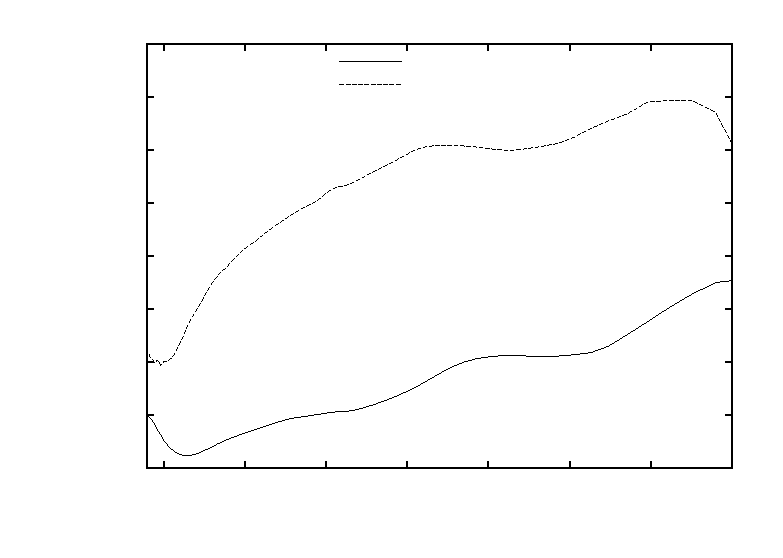
\includegraphics{CoFeSi1}}%
    \gplfronttext
  \end{picture}%
\endgroup

\caption{Spektrumn vzorku CoFeSi1}
\label{sCoFeSi1}
\end{figure}

\begin{figure}
% GNUPLOT: LaTeX picture with Postscript
\begingroup
  \makeatletter
  \providecommand\color[2][]{%
    \GenericError{(gnuplot) \space\space\space\@spaces}{%
      Package color not loaded in conjunction with
      terminal option `colourtext'%
    }{See the gnuplot documentation for explanation.%
    }{Either use 'blacktext' in gnuplot or load the package
      color.sty in LaTeX.}%
    \renewcommand\color[2][]{}%
  }%
  \providecommand\includegraphics[2][]{%
    \GenericError{(gnuplot) \space\space\space\@spaces}{%
      Package graphicx or graphics not loaded%
    }{See the gnuplot documentation for explanation.%
    }{The gnuplot epslatex terminal needs graphicx.sty or graphics.sty.}%
    \renewcommand\includegraphics[2][]{}%
  }%
  \providecommand\rotatebox[2]{#2}%
  \@ifundefined{ifGPcolor}{%
    \newif\ifGPcolor
    \GPcolortrue
  }{}%
  \@ifundefined{ifGPblacktext}{%
    \newif\ifGPblacktext
    \GPblacktexttrue
  }{}%
  % define a \g@addto@macro without @ in the name:
  \let\gplgaddtomacro\g@addto@macro
  % define empty templates for all commands taking text:
  \gdef\gplbacktext{}%
  \gdef\gplfronttext{}%
  \makeatother
  \ifGPblacktext
    % no textcolor at all
    \def\colorrgb#1{}%
    \def\colorgray#1{}%
  \else
    % gray or color?
    \ifGPcolor
      \def\colorrgb#1{\color[rgb]{#1}}%
      \def\colorgray#1{\color[gray]{#1}}%
      \expandafter\def\csname LTw\endcsname{\color{white}}%
      \expandafter\def\csname LTb\endcsname{\color{black}}%
      \expandafter\def\csname LTa\endcsname{\color{black}}%
      \expandafter\def\csname LT0\endcsname{\color[rgb]{1,0,0}}%
      \expandafter\def\csname LT1\endcsname{\color[rgb]{0,1,0}}%
      \expandafter\def\csname LT2\endcsname{\color[rgb]{0,0,1}}%
      \expandafter\def\csname LT3\endcsname{\color[rgb]{1,0,1}}%
      \expandafter\def\csname LT4\endcsname{\color[rgb]{0,1,1}}%
      \expandafter\def\csname LT5\endcsname{\color[rgb]{1,1,0}}%
      \expandafter\def\csname LT6\endcsname{\color[rgb]{0,0,0}}%
      \expandafter\def\csname LT7\endcsname{\color[rgb]{1,0.3,0}}%
      \expandafter\def\csname LT8\endcsname{\color[rgb]{0.5,0.5,0.5}}%
    \else
      % gray
      \def\colorrgb#1{\color{black}}%
      \def\colorgray#1{\color[gray]{#1}}%
      \expandafter\def\csname LTw\endcsname{\color{white}}%
      \expandafter\def\csname LTb\endcsname{\color{black}}%
      \expandafter\def\csname LTa\endcsname{\color{black}}%
      \expandafter\def\csname LT0\endcsname{\color{black}}%
      \expandafter\def\csname LT1\endcsname{\color{black}}%
      \expandafter\def\csname LT2\endcsname{\color{black}}%
      \expandafter\def\csname LT3\endcsname{\color{black}}%
      \expandafter\def\csname LT4\endcsname{\color{black}}%
      \expandafter\def\csname LT5\endcsname{\color{black}}%
      \expandafter\def\csname LT6\endcsname{\color{black}}%
      \expandafter\def\csname LT7\endcsname{\color{black}}%
      \expandafter\def\csname LT8\endcsname{\color{black}}%
    \fi
  \fi
  \setlength{\unitlength}{0.0500bp}%
  \begin{picture}(7200.00,5040.00)%
    \gplgaddtomacro\gplbacktext{%
      \csname LTb\endcsname%
      \put(1078,704){\makebox(0,0)[r]{\strut{}-0.3}}%
      \put(1078,1156){\makebox(0,0)[r]{\strut{}-0.25}}%
      \put(1078,1609){\makebox(0,0)[r]{\strut{}-0.2}}%
      \put(1078,2061){\makebox(0,0)[r]{\strut{}-0.15}}%
      \put(1078,2513){\makebox(0,0)[r]{\strut{}-0.1}}%
      \put(1078,2966){\makebox(0,0)[r]{\strut{}-0.05}}%
      \put(1078,3418){\makebox(0,0)[r]{\strut{} 0}}%
      \put(1078,3870){\makebox(0,0)[r]{\strut{} 0.05}}%
      \put(1078,4323){\makebox(0,0)[r]{\strut{} 0.1}}%
      \put(1078,4775){\makebox(0,0)[r]{\strut{} 0.15}}%
      \put(1379,484){\makebox(0,0){\strut{} 1.5}}%
      \put(2227,484){\makebox(0,0){\strut{} 2}}%
      \put(3074,484){\makebox(0,0){\strut{} 2.5}}%
      \put(3922,484){\makebox(0,0){\strut{} 3}}%
      \put(4769,484){\makebox(0,0){\strut{} 3.5}}%
      \put(5617,484){\makebox(0,0){\strut{} 4}}%
      \put(6464,484){\makebox(0,0){\strut{} 4.5}}%
      \csname LTb\endcsname%
      \put(176,2739){\rotatebox{-270}{\makebox(0,0){\strut{}Polární Kerrův jev [deg.]}}}%
      \put(4006,154){\makebox(0,0){\strut{}$E$ [eV]}}%
    }%
    \gplgaddtomacro\gplfronttext{%
      \csname LTb\endcsname%
      \put(5816,1537){\makebox(0,0)[r]{\strut{}$\theta_K$}}%
      \csname LTb\endcsname%
      \put(5816,1317){\makebox(0,0)[r]{\strut{}$\epsilon_K$}}%
      \csname LTb\endcsname%
      \put(5816,1097){\makebox(0,0)[r]{\strut{}$\theta_K$}}%
      \csname LTb\endcsname%
      \put(5816,877){\makebox(0,0)[r]{\strut{}$\epsilon_K$}}%
    }%
    \gplbacktext
    \put(0,0){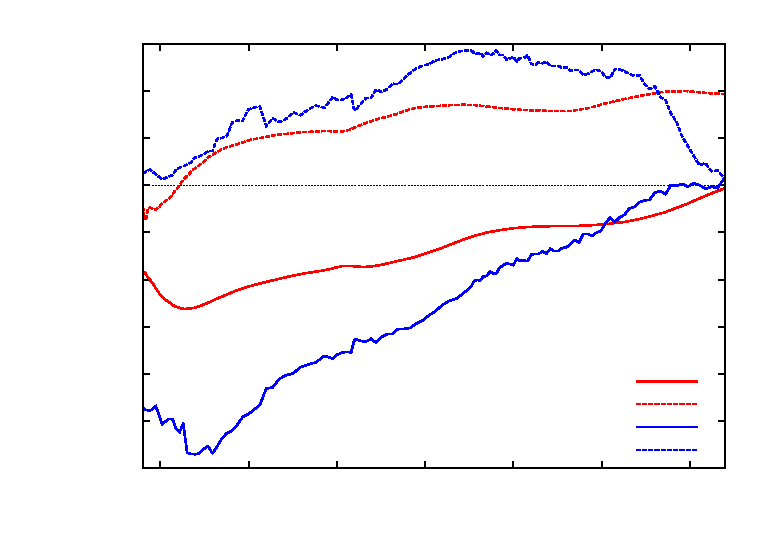
\includegraphics{CoFeSi2}}%
    \gplfronttext
  \end{picture}%
\endgroup

\caption{Spektrumn vzorku CoFeSi2}
\label{sCoFeSi2}
\end{figure}

\begin{figure}
% GNUPLOT: LaTeX picture with Postscript
\begingroup
  \makeatletter
  \providecommand\color[2][]{%
    \GenericError{(gnuplot) \space\space\space\@spaces}{%
      Package color not loaded in conjunction with
      terminal option `colourtext'%
    }{See the gnuplot documentation for explanation.%
    }{Either use 'blacktext' in gnuplot or load the package
      color.sty in LaTeX.}%
    \renewcommand\color[2][]{}%
  }%
  \providecommand\includegraphics[2][]{%
    \GenericError{(gnuplot) \space\space\space\@spaces}{%
      Package graphicx or graphics not loaded%
    }{See the gnuplot documentation for explanation.%
    }{The gnuplot epslatex terminal needs graphicx.sty or graphics.sty.}%
    \renewcommand\includegraphics[2][]{}%
  }%
  \providecommand\rotatebox[2]{#2}%
  \@ifundefined{ifGPcolor}{%
    \newif\ifGPcolor
    \GPcolortrue
  }{}%
  \@ifundefined{ifGPblacktext}{%
    \newif\ifGPblacktext
    \GPblacktexttrue
  }{}%
  % define a \g@addto@macro without @ in the name:
  \let\gplgaddtomacro\g@addto@macro
  % define empty templates for all commands taking text:
  \gdef\gplbacktext{}%
  \gdef\gplfronttext{}%
  \makeatother
  \ifGPblacktext
    % no textcolor at all
    \def\colorrgb#1{}%
    \def\colorgray#1{}%
  \else
    % gray or color?
    \ifGPcolor
      \def\colorrgb#1{\color[rgb]{#1}}%
      \def\colorgray#1{\color[gray]{#1}}%
      \expandafter\def\csname LTw\endcsname{\color{white}}%
      \expandafter\def\csname LTb\endcsname{\color{black}}%
      \expandafter\def\csname LTa\endcsname{\color{black}}%
      \expandafter\def\csname LT0\endcsname{\color[rgb]{1,0,0}}%
      \expandafter\def\csname LT1\endcsname{\color[rgb]{0,1,0}}%
      \expandafter\def\csname LT2\endcsname{\color[rgb]{0,0,1}}%
      \expandafter\def\csname LT3\endcsname{\color[rgb]{1,0,1}}%
      \expandafter\def\csname LT4\endcsname{\color[rgb]{0,1,1}}%
      \expandafter\def\csname LT5\endcsname{\color[rgb]{1,1,0}}%
      \expandafter\def\csname LT6\endcsname{\color[rgb]{0,0,0}}%
      \expandafter\def\csname LT7\endcsname{\color[rgb]{1,0.3,0}}%
      \expandafter\def\csname LT8\endcsname{\color[rgb]{0.5,0.5,0.5}}%
    \else
      % gray
      \def\colorrgb#1{\color{black}}%
      \def\colorgray#1{\color[gray]{#1}}%
      \expandafter\def\csname LTw\endcsname{\color{white}}%
      \expandafter\def\csname LTb\endcsname{\color{black}}%
      \expandafter\def\csname LTa\endcsname{\color{black}}%
      \expandafter\def\csname LT0\endcsname{\color{black}}%
      \expandafter\def\csname LT1\endcsname{\color{black}}%
      \expandafter\def\csname LT2\endcsname{\color{black}}%
      \expandafter\def\csname LT3\endcsname{\color{black}}%
      \expandafter\def\csname LT4\endcsname{\color{black}}%
      \expandafter\def\csname LT5\endcsname{\color{black}}%
      \expandafter\def\csname LT6\endcsname{\color{black}}%
      \expandafter\def\csname LT7\endcsname{\color{black}}%
      \expandafter\def\csname LT8\endcsname{\color{black}}%
    \fi
  \fi
  \setlength{\unitlength}{0.0500bp}%
  \begin{picture}(7200.00,5040.00)%
    \gplgaddtomacro\gplbacktext{%
      \csname LTb\endcsname%
      \put(946,704){\makebox(0,0)[r]{\strut{}-0.6}}%
      \put(946,1383){\makebox(0,0)[r]{\strut{}-0.4}}%
      \put(946,2061){\makebox(0,0)[r]{\strut{}-0.2}}%
      \put(946,2740){\makebox(0,0)[r]{\strut{} 0}}%
      \put(946,3418){\makebox(0,0)[r]{\strut{} 0.2}}%
      \put(946,4097){\makebox(0,0)[r]{\strut{} 0.4}}%
      \put(946,4775){\makebox(0,0)[r]{\strut{} 0.6}}%
      \put(1257,484){\makebox(0,0){\strut{} 1.5}}%
      \put(2151,484){\makebox(0,0){\strut{} 2}}%
      \put(3046,484){\makebox(0,0){\strut{} 2.5}}%
      \put(3941,484){\makebox(0,0){\strut{} 3}}%
      \put(4835,484){\makebox(0,0){\strut{} 3.5}}%
      \put(5730,484){\makebox(0,0){\strut{} 4}}%
      \put(6624,484){\makebox(0,0){\strut{} 4.5}}%
      \csname LTb\endcsname%
      \put(176,2739){\rotatebox{-270}{\makebox(0,0){\strut{}Polární Kerrův jev [deg.]}}}%
      \put(3940,154){\makebox(0,0){\strut{}$E$ [eV]}}%
    }%
    \gplgaddtomacro\gplfronttext{%
      \csname LTb\endcsname%
      \put(5816,4602){\makebox(0,0)[r]{\strut{}$\theta_K$}}%
      \csname LTb\endcsname%
      \put(5816,4382){\makebox(0,0)[r]{\strut{}$\epsilon_K$}}%
      \csname LTb\endcsname%
      \put(5816,4162){\makebox(0,0)[r]{\strut{}$\theta_K$}}%
      \csname LTb\endcsname%
      \put(5816,3942){\makebox(0,0)[r]{\strut{}$\epsilon_K$}}%
    }%
    \gplbacktext
    \put(0,0){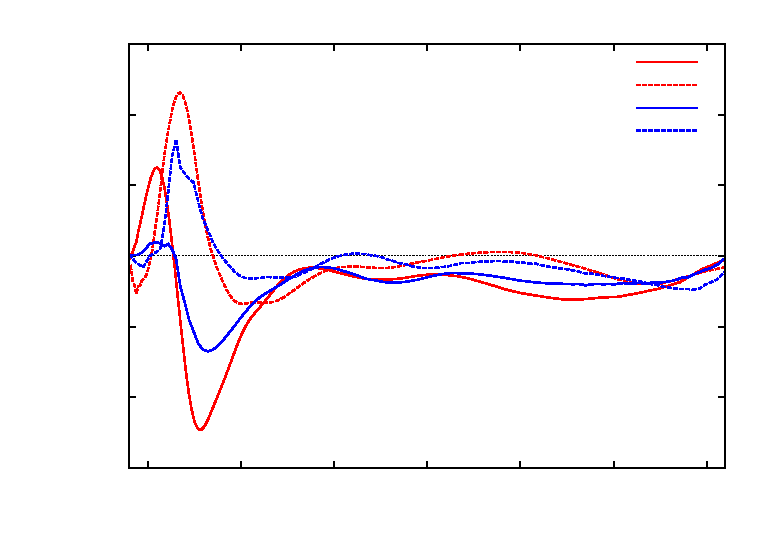
\includegraphics{CoF-RT-A750}}%
    \gplfronttext
  \end{picture}%
\endgroup

\caption{Spektrumn vzorku CoF-RT-A750}
\label{sCoF-RT-A750}
\end{figure}

\begin{figure}
% GNUPLOT: LaTeX picture with Postscript
\begingroup
  \makeatletter
  \providecommand\color[2][]{%
    \GenericError{(gnuplot) \space\space\space\@spaces}{%
      Package color not loaded in conjunction with
      terminal option `colourtext'%
    }{See the gnuplot documentation for explanation.%
    }{Either use 'blacktext' in gnuplot or load the package
      color.sty in LaTeX.}%
    \renewcommand\color[2][]{}%
  }%
  \providecommand\includegraphics[2][]{%
    \GenericError{(gnuplot) \space\space\space\@spaces}{%
      Package graphicx or graphics not loaded%
    }{See the gnuplot documentation for explanation.%
    }{The gnuplot epslatex terminal needs graphicx.sty or graphics.sty.}%
    \renewcommand\includegraphics[2][]{}%
  }%
  \providecommand\rotatebox[2]{#2}%
  \@ifundefined{ifGPcolor}{%
    \newif\ifGPcolor
    \GPcolorfalse
  }{}%
  \@ifundefined{ifGPblacktext}{%
    \newif\ifGPblacktext
    \GPblacktexttrue
  }{}%
  % define a \g@addto@macro without @ in the name:
  \let\gplgaddtomacro\g@addto@macro
  % define empty templates for all commands taking text:
  \gdef\gplbacktext{}%
  \gdef\gplfronttext{}%
  \makeatother
  \ifGPblacktext
    % no textcolor at all
    \def\colorrgb#1{}%
    \def\colorgray#1{}%
  \else
    % gray or color?
    \ifGPcolor
      \def\colorrgb#1{\color[rgb]{#1}}%
      \def\colorgray#1{\color[gray]{#1}}%
      \expandafter\def\csname LTw\endcsname{\color{white}}%
      \expandafter\def\csname LTb\endcsname{\color{black}}%
      \expandafter\def\csname LTa\endcsname{\color{black}}%
      \expandafter\def\csname LT0\endcsname{\color[rgb]{1,0,0}}%
      \expandafter\def\csname LT1\endcsname{\color[rgb]{0,1,0}}%
      \expandafter\def\csname LT2\endcsname{\color[rgb]{0,0,1}}%
      \expandafter\def\csname LT3\endcsname{\color[rgb]{1,0,1}}%
      \expandafter\def\csname LT4\endcsname{\color[rgb]{0,1,1}}%
      \expandafter\def\csname LT5\endcsname{\color[rgb]{1,1,0}}%
      \expandafter\def\csname LT6\endcsname{\color[rgb]{0,0,0}}%
      \expandafter\def\csname LT7\endcsname{\color[rgb]{1,0.3,0}}%
      \expandafter\def\csname LT8\endcsname{\color[rgb]{0.5,0.5,0.5}}%
    \else
      % gray
      \def\colorrgb#1{\color{black}}%
      \def\colorgray#1{\color[gray]{#1}}%
      \expandafter\def\csname LTw\endcsname{\color{white}}%
      \expandafter\def\csname LTb\endcsname{\color{black}}%
      \expandafter\def\csname LTa\endcsname{\color{black}}%
      \expandafter\def\csname LT0\endcsname{\color{black}}%
      \expandafter\def\csname LT1\endcsname{\color{black}}%
      \expandafter\def\csname LT2\endcsname{\color{black}}%
      \expandafter\def\csname LT3\endcsname{\color{black}}%
      \expandafter\def\csname LT4\endcsname{\color{black}}%
      \expandafter\def\csname LT5\endcsname{\color{black}}%
      \expandafter\def\csname LT6\endcsname{\color{black}}%
      \expandafter\def\csname LT7\endcsname{\color{black}}%
      \expandafter\def\csname LT8\endcsname{\color{black}}%
    \fi
  \fi
  \setlength{\unitlength}{0.0500bp}%
  \begin{picture}(7200.00,5040.00)%
    \gplgaddtomacro\gplbacktext{%
      \csname LTb\endcsname%
      \put(1078,704){\makebox(0,0)[r]{\strut{}-0.4}}%
      \put(1078,1213){\makebox(0,0)[r]{\strut{}-0.3}}%
      \put(1078,1722){\makebox(0,0)[r]{\strut{}-0.2}}%
      \put(1078,2231){\makebox(0,0)[r]{\strut{}-0.1}}%
      \put(1078,2739){\makebox(0,0)[r]{\strut{} 0}}%
      \put(1078,3248){\makebox(0,0)[r]{\strut{} 0.1}}%
      \put(1078,3757){\makebox(0,0)[r]{\strut{} 0.2}}%
      \put(1078,4266){\makebox(0,0)[r]{\strut{} 0.3}}%
      \put(1078,4775){\makebox(0,0)[r]{\strut{} 0.4}}%
      \put(1367,484){\makebox(0,0){\strut{} 1.5}}%
      \put(2153,484){\makebox(0,0){\strut{} 2}}%
      \put(2939,484){\makebox(0,0){\strut{} 2.5}}%
      \put(3725,484){\makebox(0,0){\strut{} 3}}%
      \put(4511,484){\makebox(0,0){\strut{} 3.5}}%
      \put(5297,484){\makebox(0,0){\strut{} 4}}%
      \put(6083,484){\makebox(0,0){\strut{} 4.5}}%
      \put(6869,484){\makebox(0,0){\strut{} 5}}%
      \put(308,2739){\rotatebox{-270}{\makebox(0,0){\strut{}Polární Kerrův jev [deg.]}}}%
      \put(4039,154){\makebox(0,0){\strut{}$E$/eV}}%
    }%
    \gplgaddtomacro\gplfronttext{%
      \csname LTb\endcsname%
      \put(5882,4602){\makebox(0,0)[r]{\strut{}$\theta^1_K$}}%
      \csname LTb\endcsname%
      \put(5882,4382){\makebox(0,0)[r]{\strut{}$\epsilon^1_K$}}%
      \csname LTb\endcsname%
      \put(5882,4162){\makebox(0,0)[r]{\strut{}$\theta^2_K$}}%
      \csname LTb\endcsname%
      \put(5882,3942){\makebox(0,0)[r]{\strut{}$\epsilon^2_K$}}%
    }%
    \gplbacktext
    \put(0,0){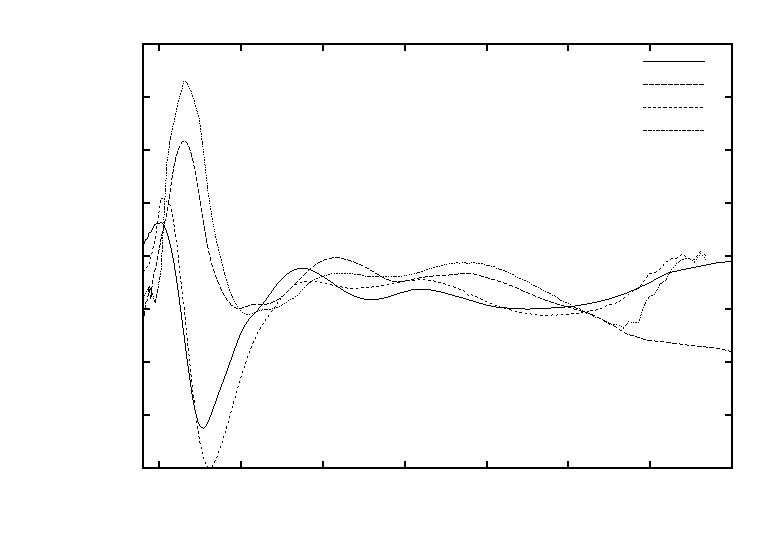
\includegraphics{grafy/CoF-RT-A1100}}%
    \gplfronttext
  \end{picture}%
\endgroup

\caption{Spektrumn vzorku CoF-RT-A1100}
\label{sCoF-RT-A1100}
\end{figure}


% Ukázka použití některých konstrukcí LateXu (odkomentujte, chcete-li)
% %%% Ukázka použití některých konstrukcí LaTeXu

\subsection{Ukázka \LaTeX{}u}
\label{ssec:ukazka}

V~této krátké části ukážeme použití několika základních konstrukcí \LaTeX{}u,
které by se vám mohly při psaní práce hodit.

Třeba odrážky:

\begin{itemize}
\item Logo Matfyzu vidíme na obrázku~\ref{fig:mff}.
\item Tato subsekce má číslo~\ref{ssec:ukazka}.
\item Odkaz na literaturu~\cite{lamport94}.
\end{itemize}

Druhy pomlček:
červeno-černý (krátká),
strana 16--22 (střední),
$45-44$ (minus),
a~toto je --- jak se asi dalo čekat --- vložená věta ohraničená dlouhými pomlčkami.
(Všimněte si, že jsme za \verb|a| napsali vlnovku místo mezery: to aby se
tam nemohl rozdělit řádek.)

% Makro na české uvozovky (novější verze LaTeXu ho už mají zabudované)
\newcommand{\uv}[1]{\quotedblbase #1\textquotedblleft}
\uv{České uvozovky.}

\newtheorem{theorem}{Věta}
\newtheorem*{define}{Definice}	% Definice nečíslujeme, proto "*"

\begin{define}
{\sl Strom} je souvislý graf bez kružnic.
\end{define}

\begin{theorem}
Tato věta neplatí.
\end{theorem}

\begin{proof}
Neplatné věty nemají důkaz.
\end{proof}

\begin{figure}
	\centering
	
\includegraphics[width=30mm]{../img/logo.eps}
	\caption{Logo MFF UK}
	\label{fig:mff}
\end{figure}


\chapter*{Závěr}
\addcontentsline{toc}{chapter}{Závěr}

Náplní této práce bylo zkoumání fyzikálních vlastností magnetooptických nanostruktur pomocí různých metod měření magnetooptických jevů. Kvůli tomu byl nejprve rozebrán popis polarizace světla 
a její vývoj v prostoru za pomoci Jonesova formalismu, v rámci čehož byly zavedeny i magnetooptické veličiny. Tento formalizmus 
byl posléze využit pro popis teoretického podkladu experimentálních metod, kterými jsme se zabývaly.

Následně byla vyložena teorie týkající se anizotropních látek, jejíž závěrem bylo teoretické určení magnetooptických veličin pro jednoduchou 
vrstu. Toho bylo využito pro výpočet spekter tenkých vrstev La$_{2/3}$Sr$_{1/3}$MnO$_3$, která byla srovnána s naměřenými hodnotami. 
Pro zbytek vzorků jsme neměli potřebné materiálové konstanty nutné pro výpočet.

Dále jsme se zabývali samotnými experimentálními metodami měření Kerrova jevu. K tomuto tématu byly uvedeny dvě různé metody. U každé znich 
jsme rozebrali teoretický model a u metody zkřížených polarizátorů jsme na jeho základě jsme postavili celou aparaturu. 
Znalosti modulační metody byly využity k modernizaci ovládacího programu této metody.

Na závěr byly změřeny konkrétní vzorky ze zástupců tří odlišných skupin materiálů a na nich porovnány účinnosti obou metod. Jako lepší metoda
se prokázala metoda se zkříženými polarizátory. Mezi její hlavní přednosti patří výrazně kratší čas měření, lepší spektrální rozlišení, 
konstrukční jednoduchost, variabilita a spolehlivost. Za zmínku také stojí výrazně nížší pořizovací náklady, a to především kvůli menšímu počtu 
zařízení, optických prvků a slabšímu zdroji světla.


%%% Seznam použité literatury
%%% Seznam použité literatury je zpracován podle platných standardů. Povinnou citační
%%% normou pro bakalářskou práci je ISO 690. Jména časopisů lze uvádět zkráceně, ale jen
%%% v kodifikované podobě. Všechny použité zdroje a prameny musí být řádně citovány.

\def\bibname{Seznam použité literatury}
\begin{thebibliography}{99}
\addcontentsline{toc}{chapter}{\bibname}

%\bibitem{lamport94}
%  {\sc Lamport,} Leslie.
%  \emph{\LaTeX: A Document Preparation System}.
%  2. vydání.
%  Massachusetts: Addison Wesley, 1994.
%  ISBN 0-201-52983-1.

\end{thebibliography}


%%% Tabulky v bakalářské práci, existují-li.
%\chapwithtoc{Seznam tabulek}

%%% Použité zkratky v bakalářské práci, existují-li, včetně jejich vysvětlení.
%\chapwithtoc{Seznam použitých zkratek}

%%% Přílohy k bakalářské práci, existují-li (různé dodatky jako výpisy programů,
%%% diagramy apod.). Každá příloha musí být alespoň jednou odkazována z vlastního
%%% textu práce. Přílohy se číslují.
%\chapwithtoc{Přílohy}

\openright
\end{document}
